\section{一维离散映射系统:帐篷映射}
帐篷映射(Tent Map),是一个一维分段的线性映射,因其函数图像类似帐篷而得名。其广泛运用在混沌加密系统中,并且在混沌扩频码的产生、混沌加密系统构造和混沌优选算法的实现中也经常被使用。

\subsection{帐篷映射的动力学}

帐篷映射是定义在$x\in [0,1]$上的一维离散映射:
\begin{equation}
    x_{n+1}=f(x_n)=
    \begin{cases}
        \begin{aligned}
            &\dfrac{x_n}{\alpha}&,\ x\in [0,\alpha)\\
            &\dfrac{1-x_n}{1-\alpha}&,\ x\in [\alpha,1]
        \end{aligned}
    \end{cases},\ n=1,2,3,\cdots
\end{equation}
其中$0<\alpha<1$,在$\alpha=\frac{1}{2}$的特殊情况下,帐篷映射可以写为
\begin{equation}
    x_{n+1}=f(x_n)=1-2|x-\frac{1}{2}|=
    \begin{cases}
        \begin{aligned}
            &2x_n&,\ x\in [0,\frac{1}{2})\\
            &2-2x_n&,\ x\in [\frac{1}{2},1]
        \end{aligned}
    \end{cases},\ n=1,2,3,\cdots
\end{equation}

帐篷映射存在两个不动点:$x_1^*=0$和$x_2^*=\frac{2}{3}$。帐篷映射在其参数范围内是一个混沌映射,并且具有均匀的分布函数和良好的相关性。帐篷映射的相图描述了相空间的映射关系$x_n\rightarrow x_{n+1}$:
\begin{figure}
	\centering
	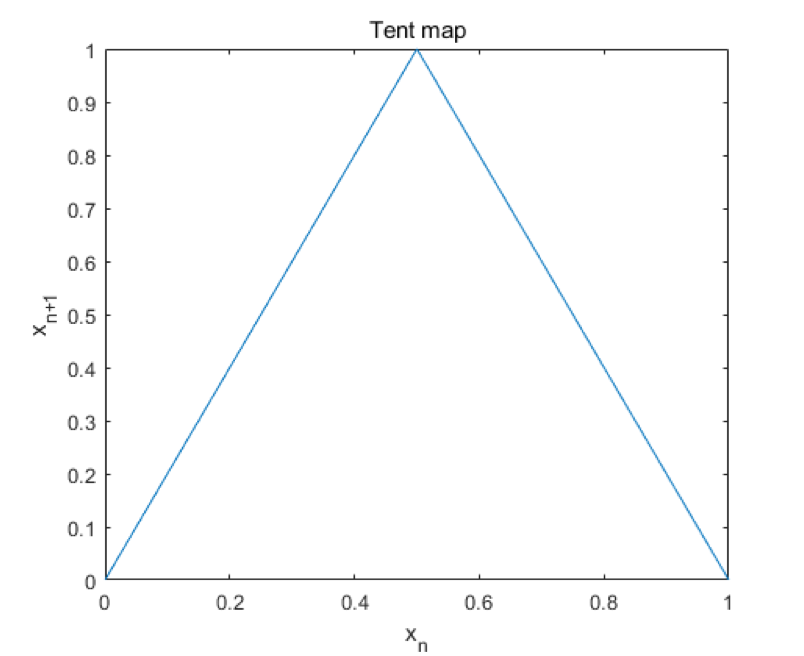
\includegraphics[scale=0.6]{tent_phase.png}
    \caption{帐篷映射的相图($\alpha=\frac{1}{2}$)}
    \label{fig:tent_pha}
\end{figure}

帐篷映射的动力学过程可以看作是在相空间$(0,1)$上的点拉伸再折叠的过程
\begin{figure}
	\centering
	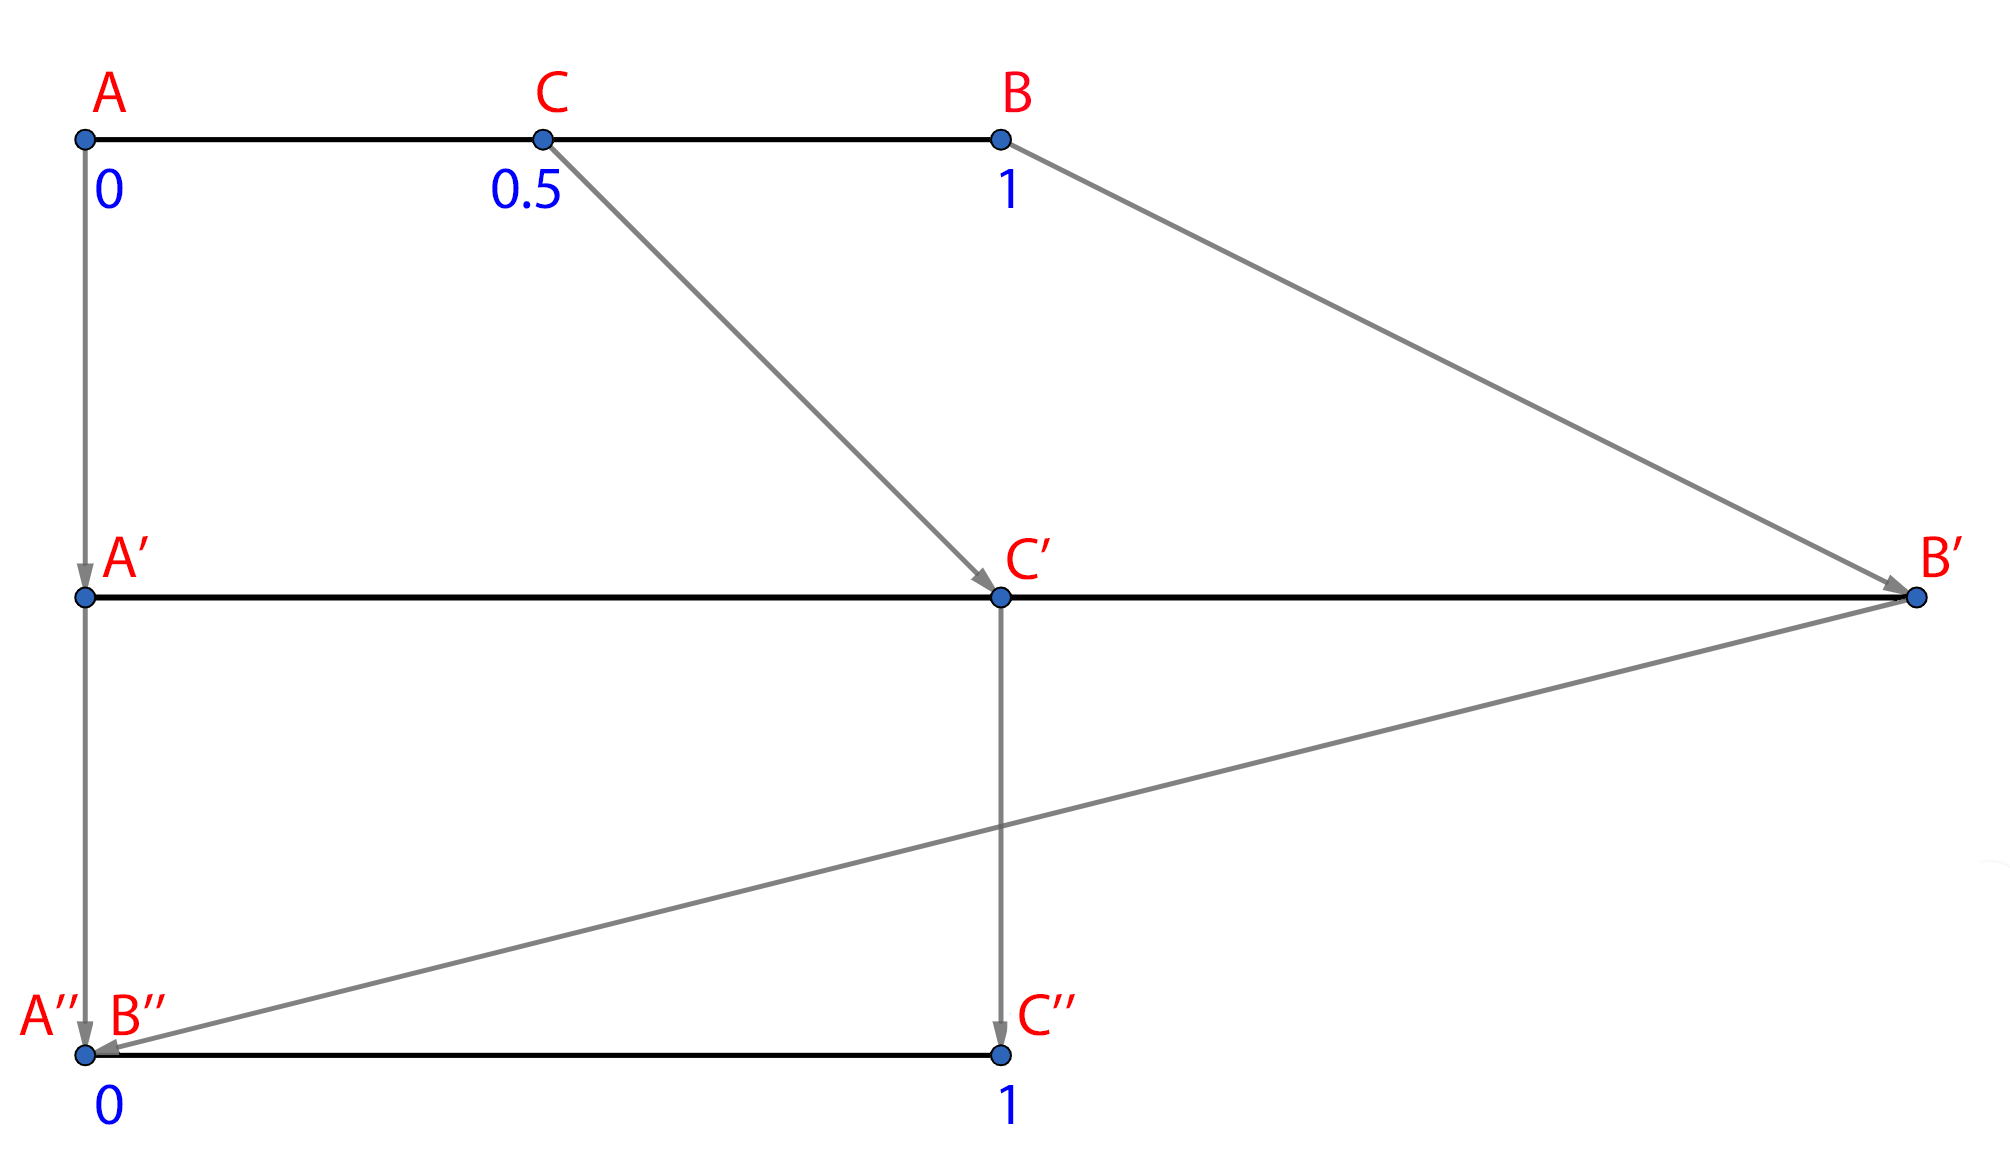
\includegraphics[scale=0.15]{tent/tent_dynamic.png}
    \caption{帐篷映射的映射过程}
    \label{fig:tent_dyna}
\end{figure}
如图\ref{fig:tent_dyna},帐篷映射可以看作两次映射的复合,第一次映射将$AB$区间上的点拉伸为$A'B'$,相空间从$(0,1)$拉伸到$(0,2)$,点$0$、$0.5$、$1$分别映射为$0$、$1$、$2$;第二次映射将$A'B'$区间上的点拉伸为$A''B''$,相空间从$(0,2)$压缩到$(0,1)$,点$0$、$1$、$2$分别映射为$0$、$1$、$0$。两次映射的拉伸与折叠过程完成了相空间$(0,1)$到其自身的映射。在该过程中,存在一些关键的“转折点”,如第一次映射的$x=0.5$与第二次映射的$x=1$,且相空间的性质随这些点呈对称分布。

\subsection{帐篷映射的Koopman算符本征函数}
\subsubsection{正交完备基函数空间}
\begin{figure}
    \centering
    \subfloat[矩形窗基函数]{
      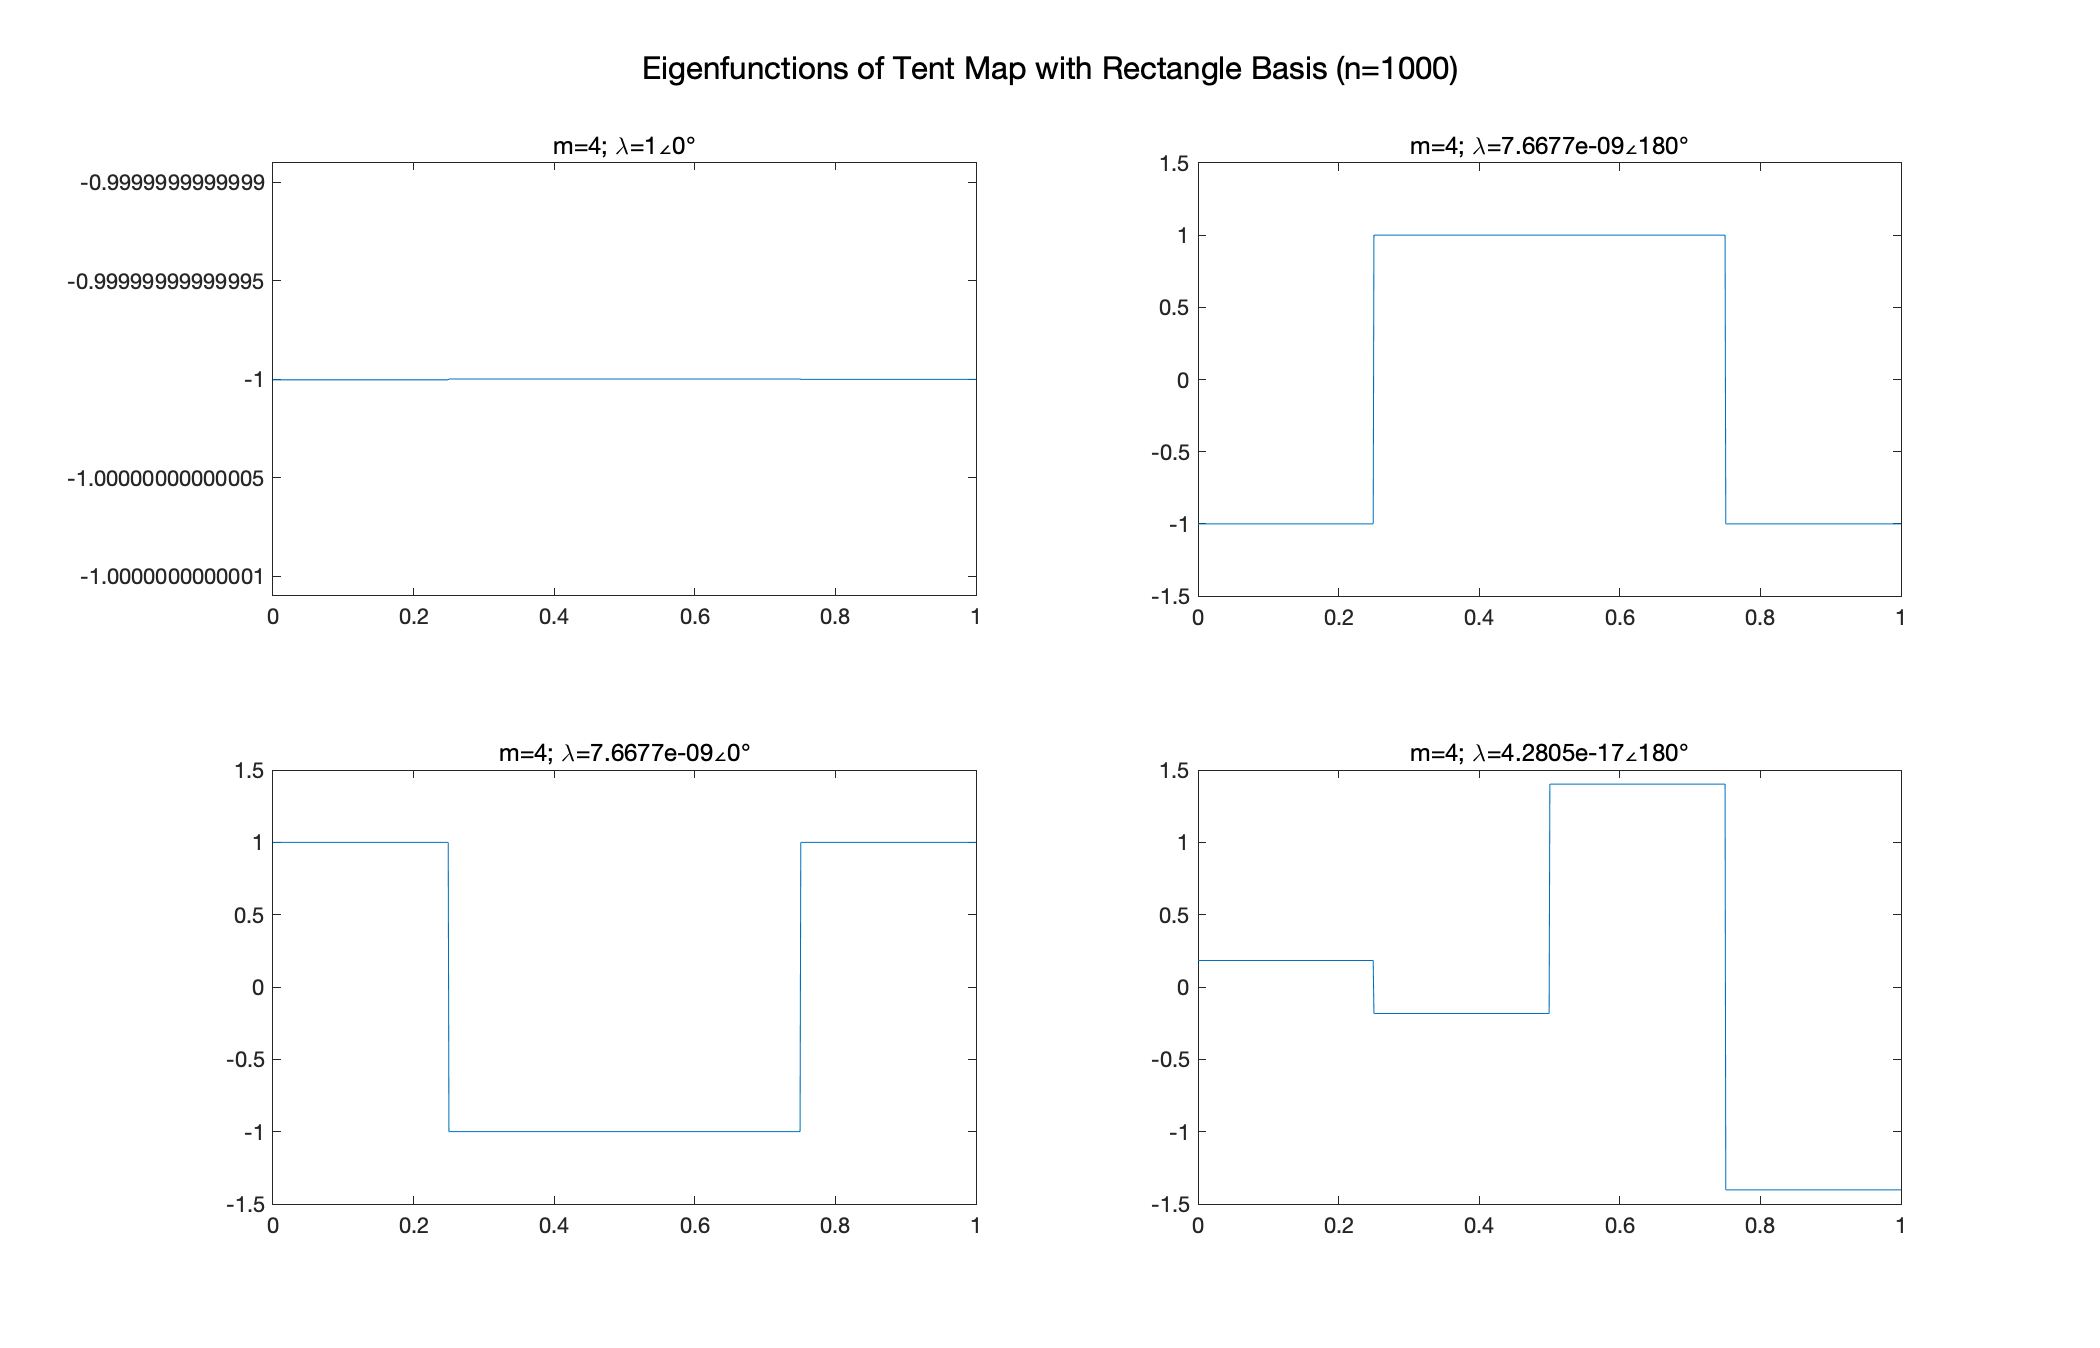
\includegraphics[scale=0.2]{tent/Tent_eigen_Rectangle_n1000_m4}}
    \subfloat[高斯基函数]{
      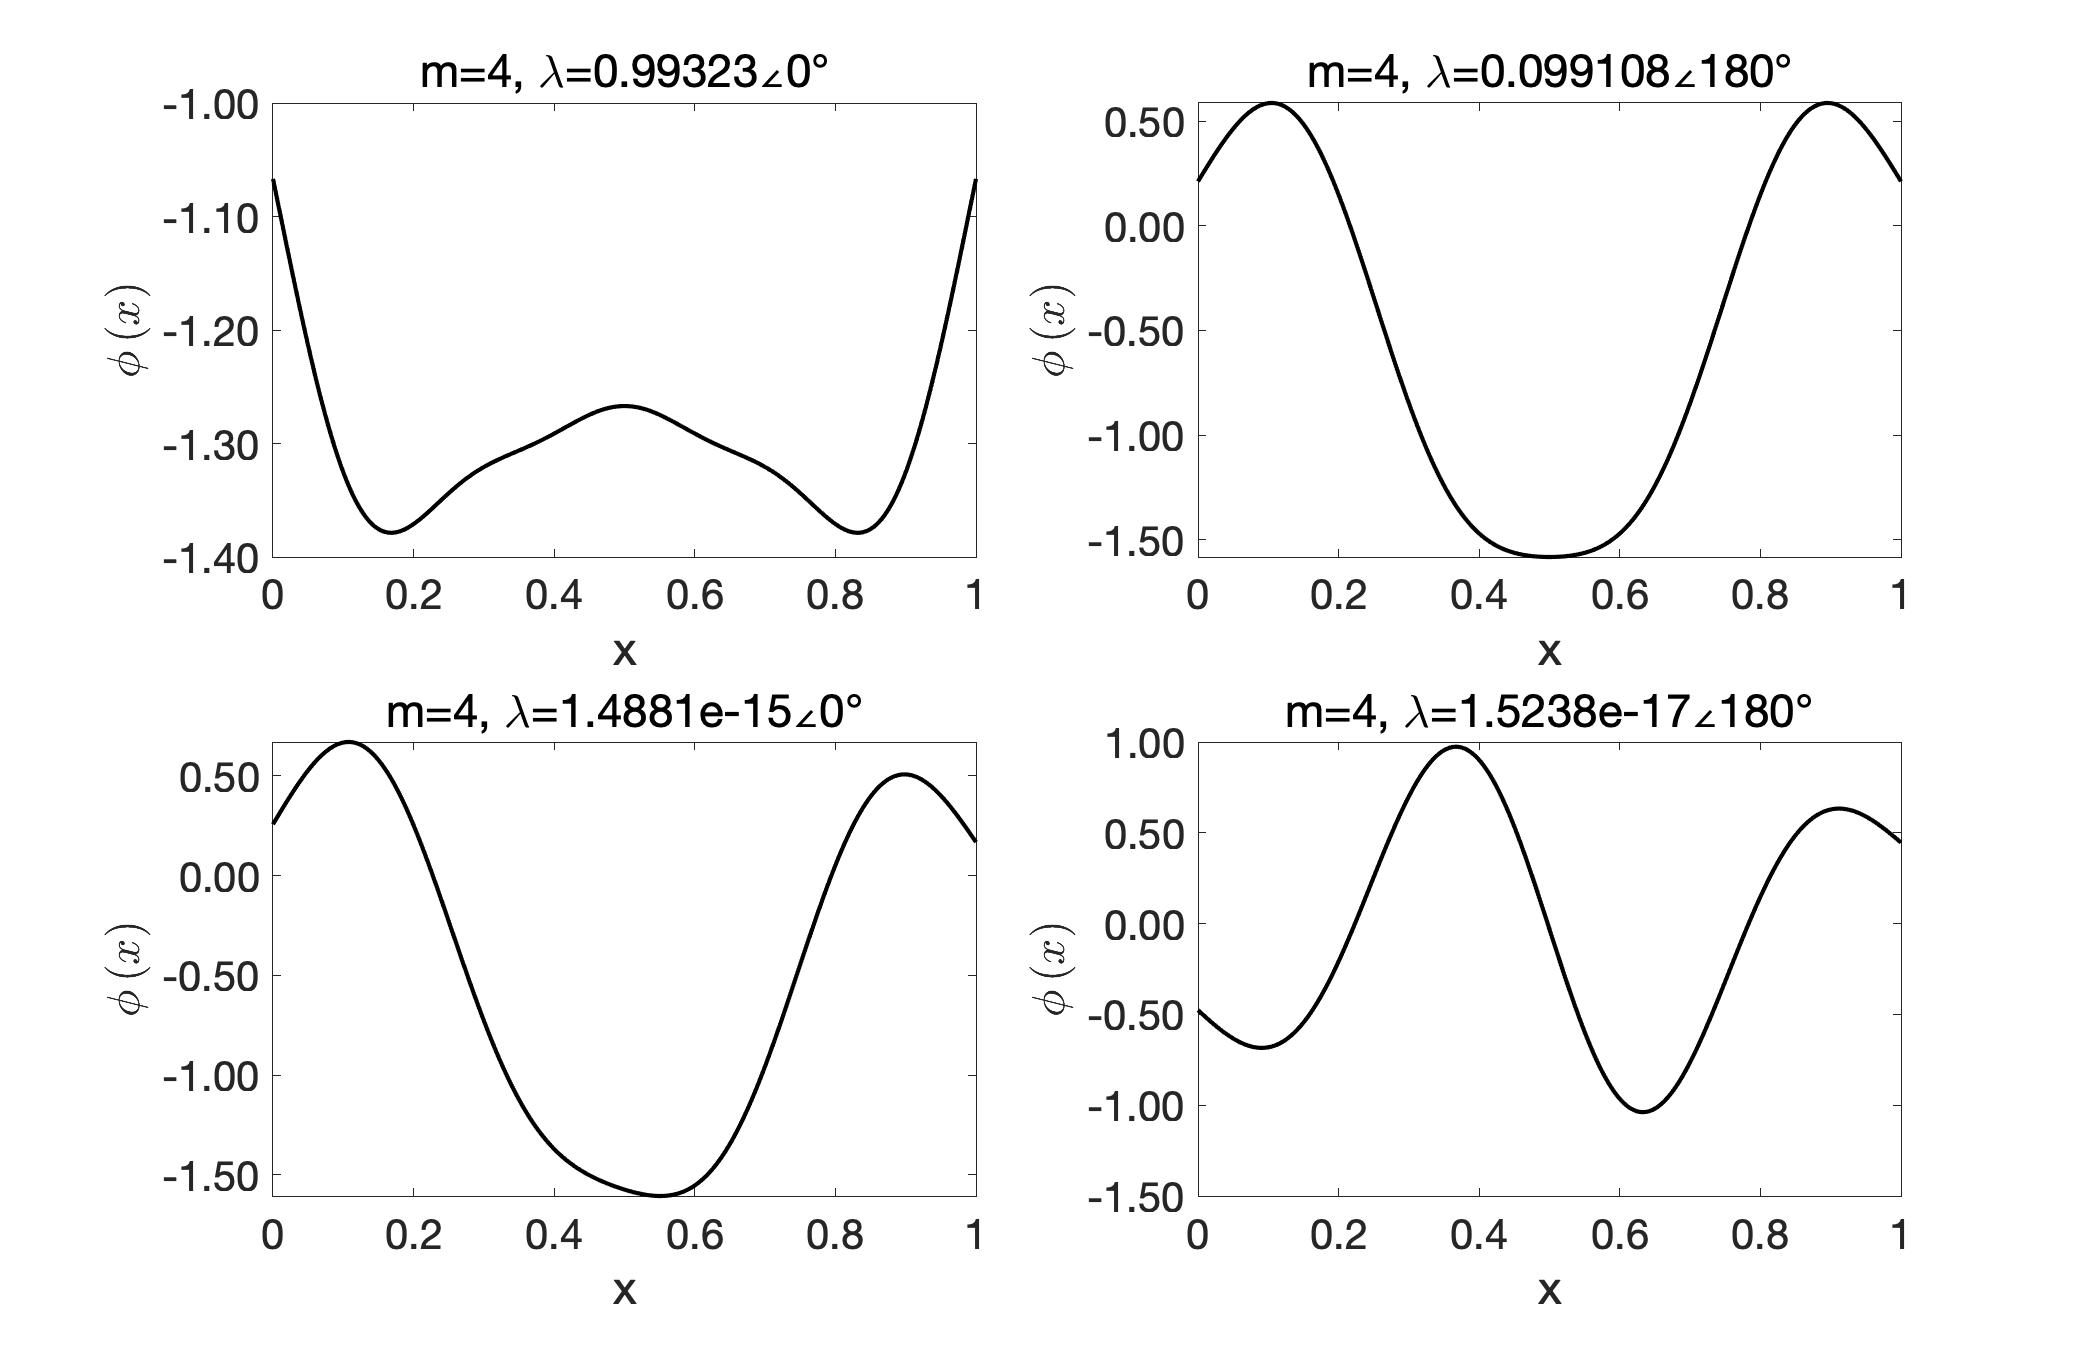
\includegraphics[scale=0.2]{tent/Tent_eigen_Gauss_n1000_m4}}
      \\
    \subfloat[傅里叶基函数]{
      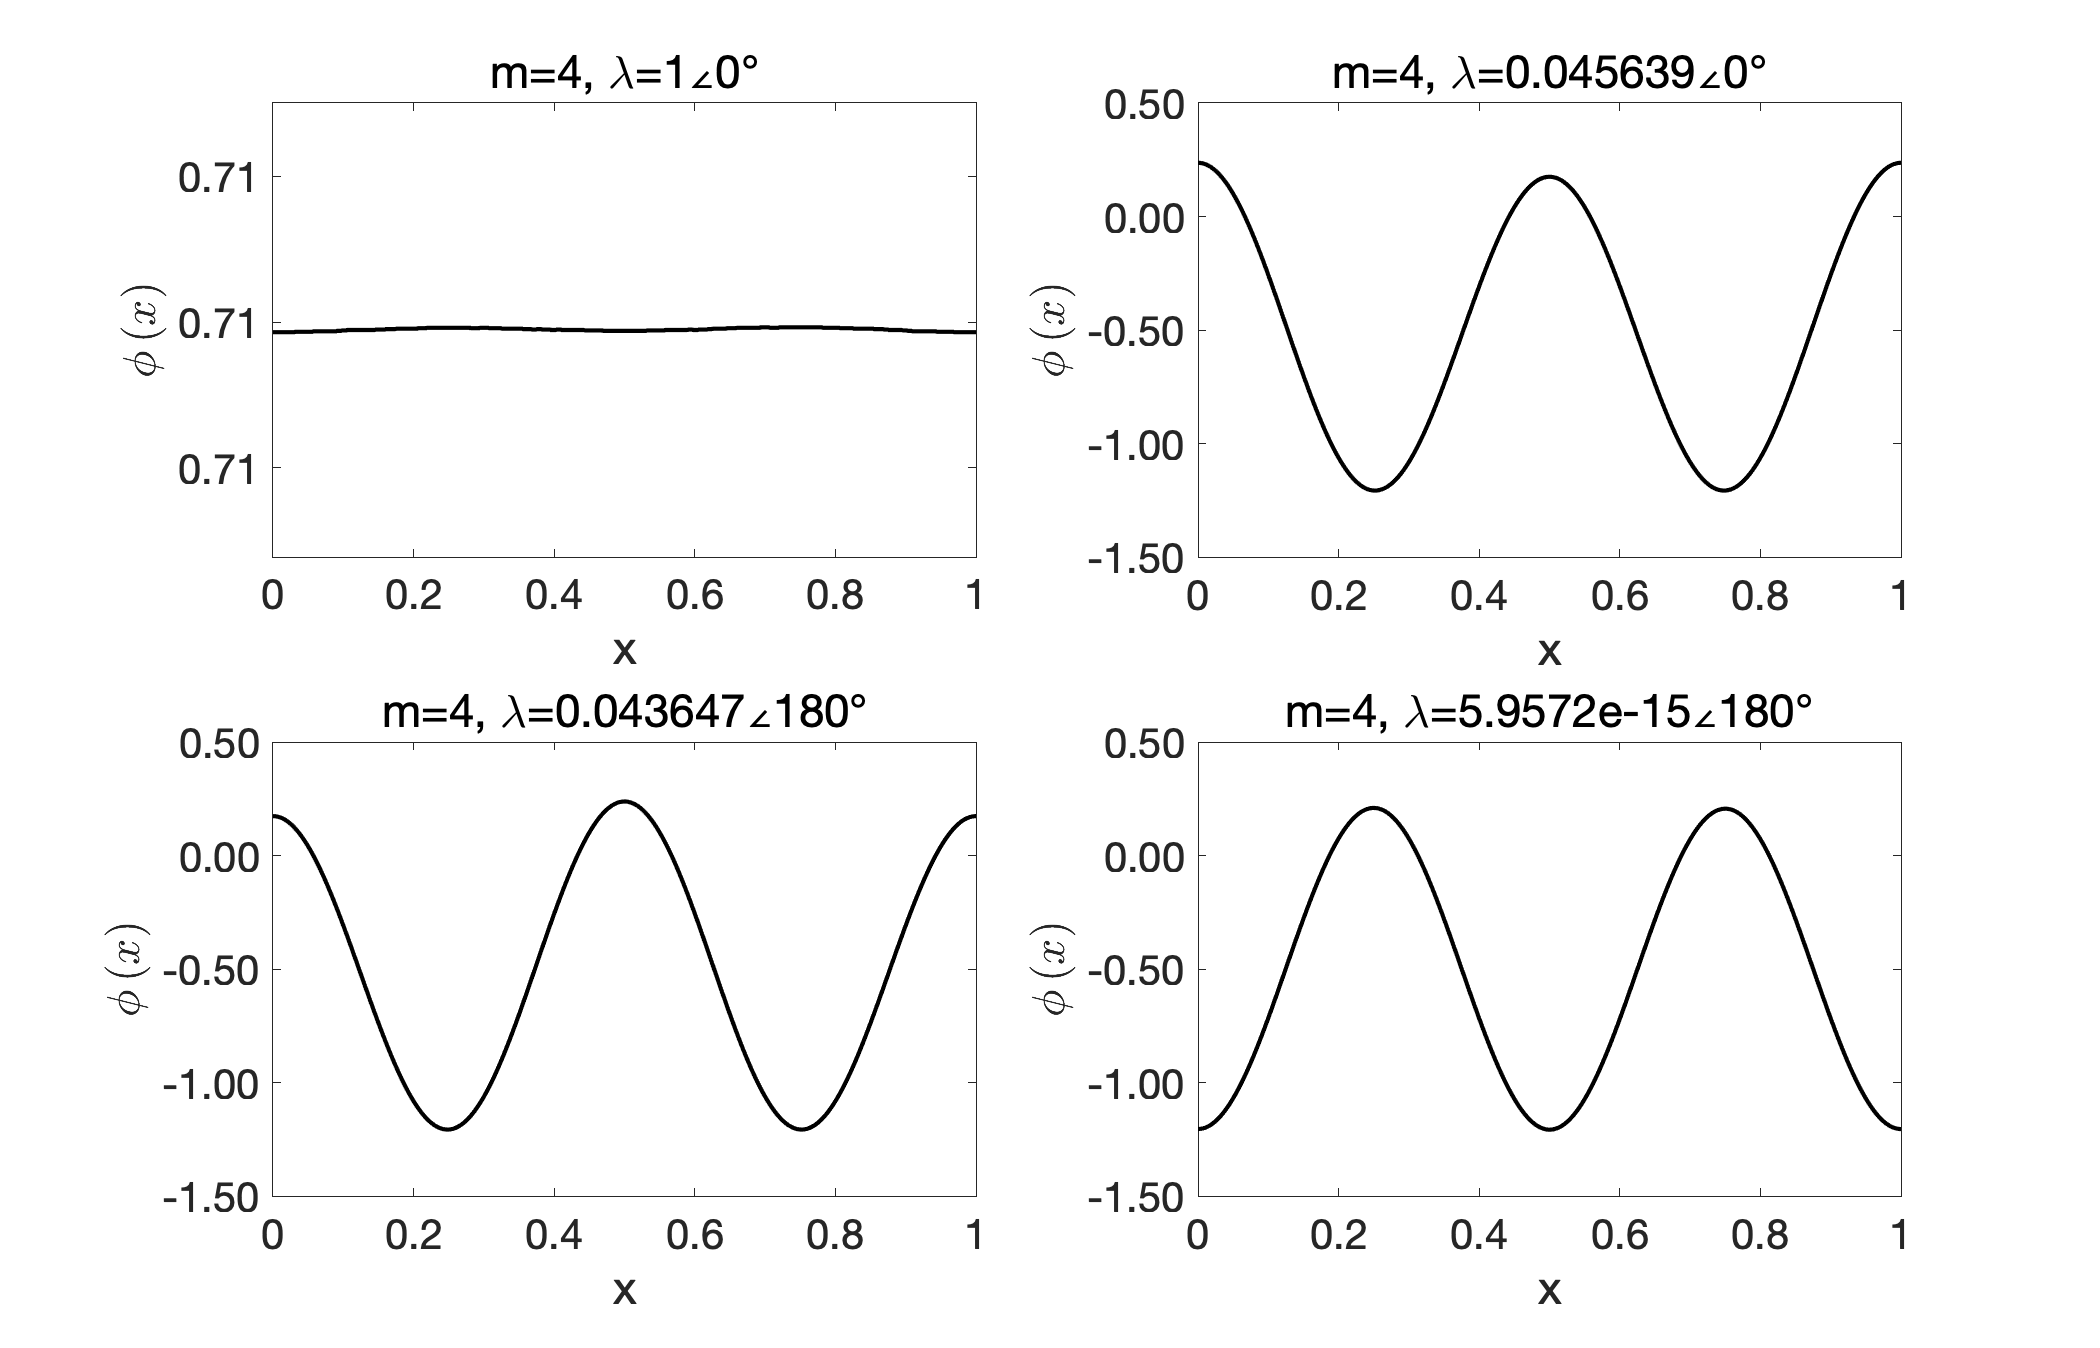
\includegraphics[scale=0.2]{tent/Tent_eigen_Fourier_n1000_m4}}
    \subfloat[勒让德基函数]{
      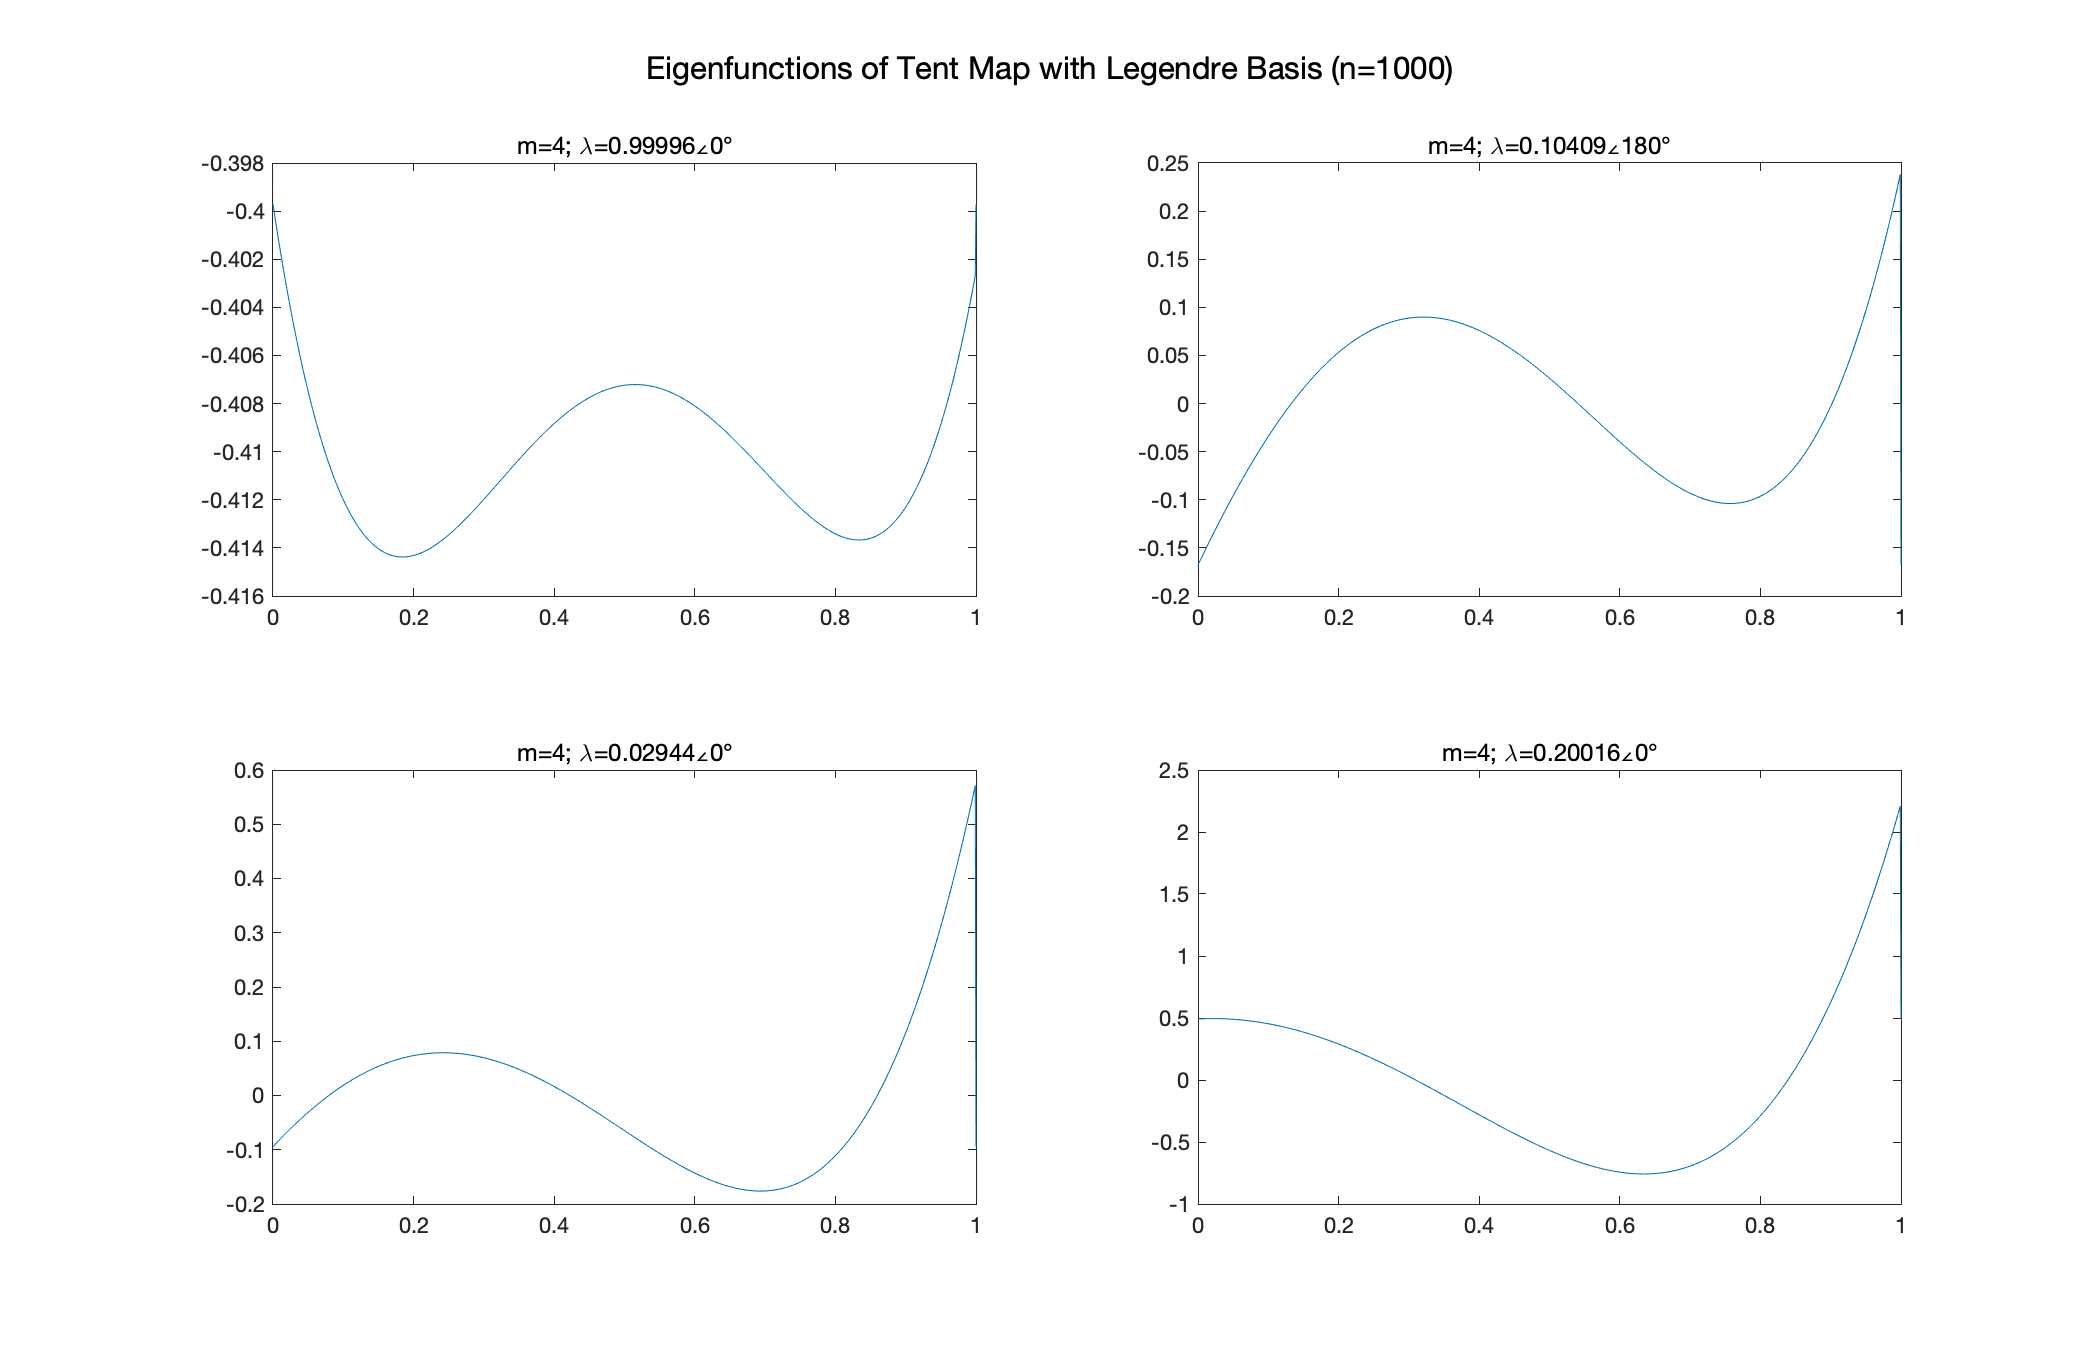
\includegraphics[scale=0.2]{tent/Tent_eigen_Legendre_n1000_m4}}
    \caption{四种基函数下帐篷映射的本征函数($m=4$)}
\end{figure}
\begin{figure}
  \centering
  \subfloat[矩形窗基函数]{
    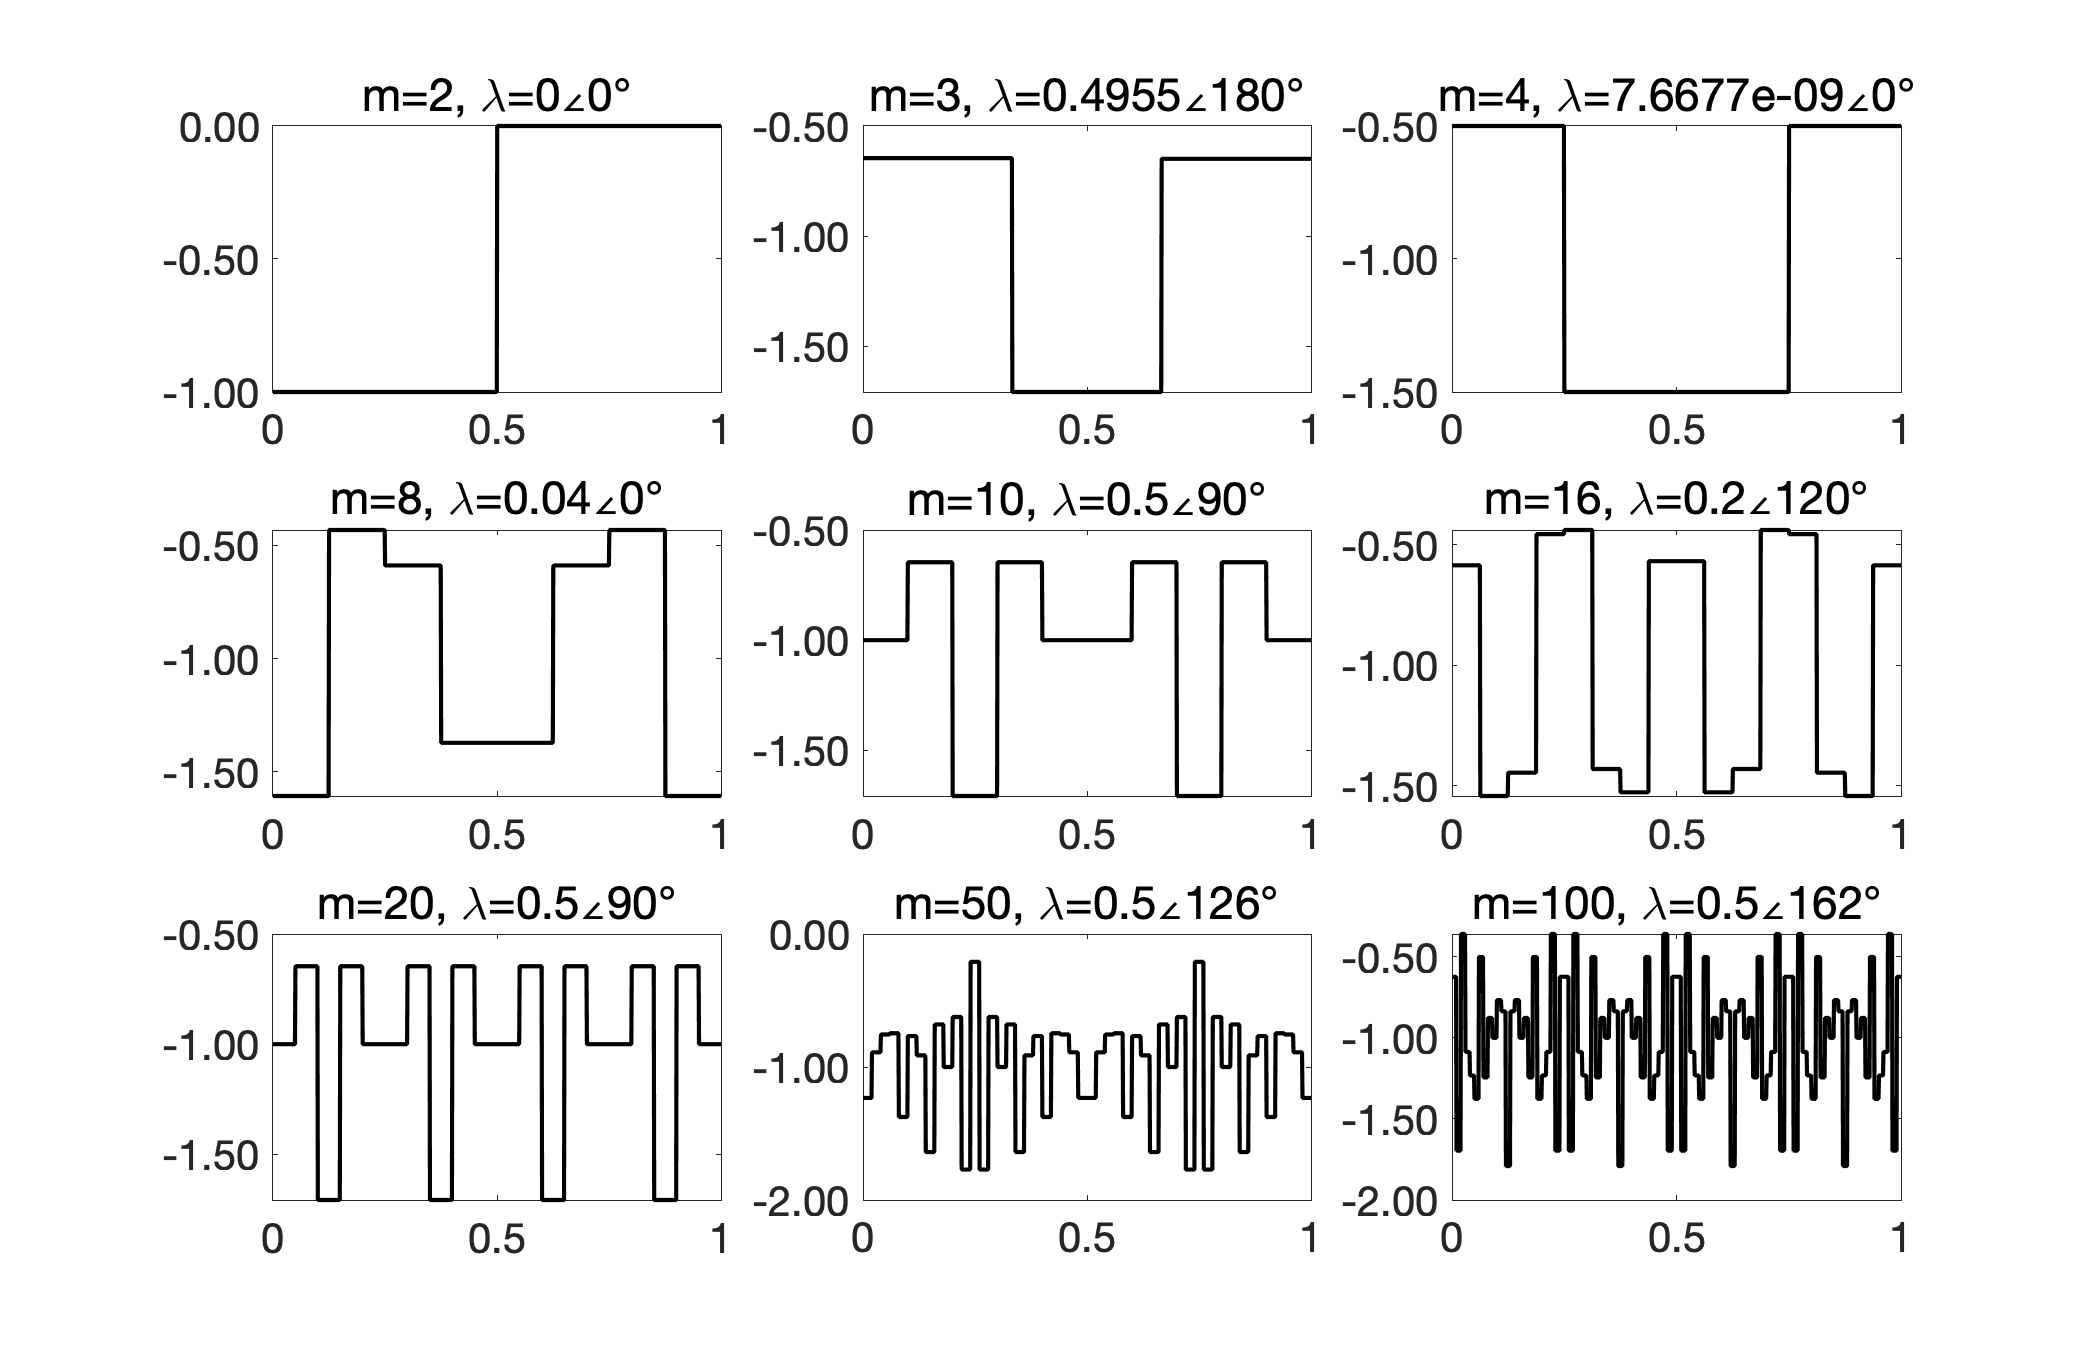
\includegraphics[scale=0.2]{tent/Tent_eigen_Rectangle_n1000_m2-3-4-8-10-16-20-50-100}}
  \subfloat[高斯基函数]{
    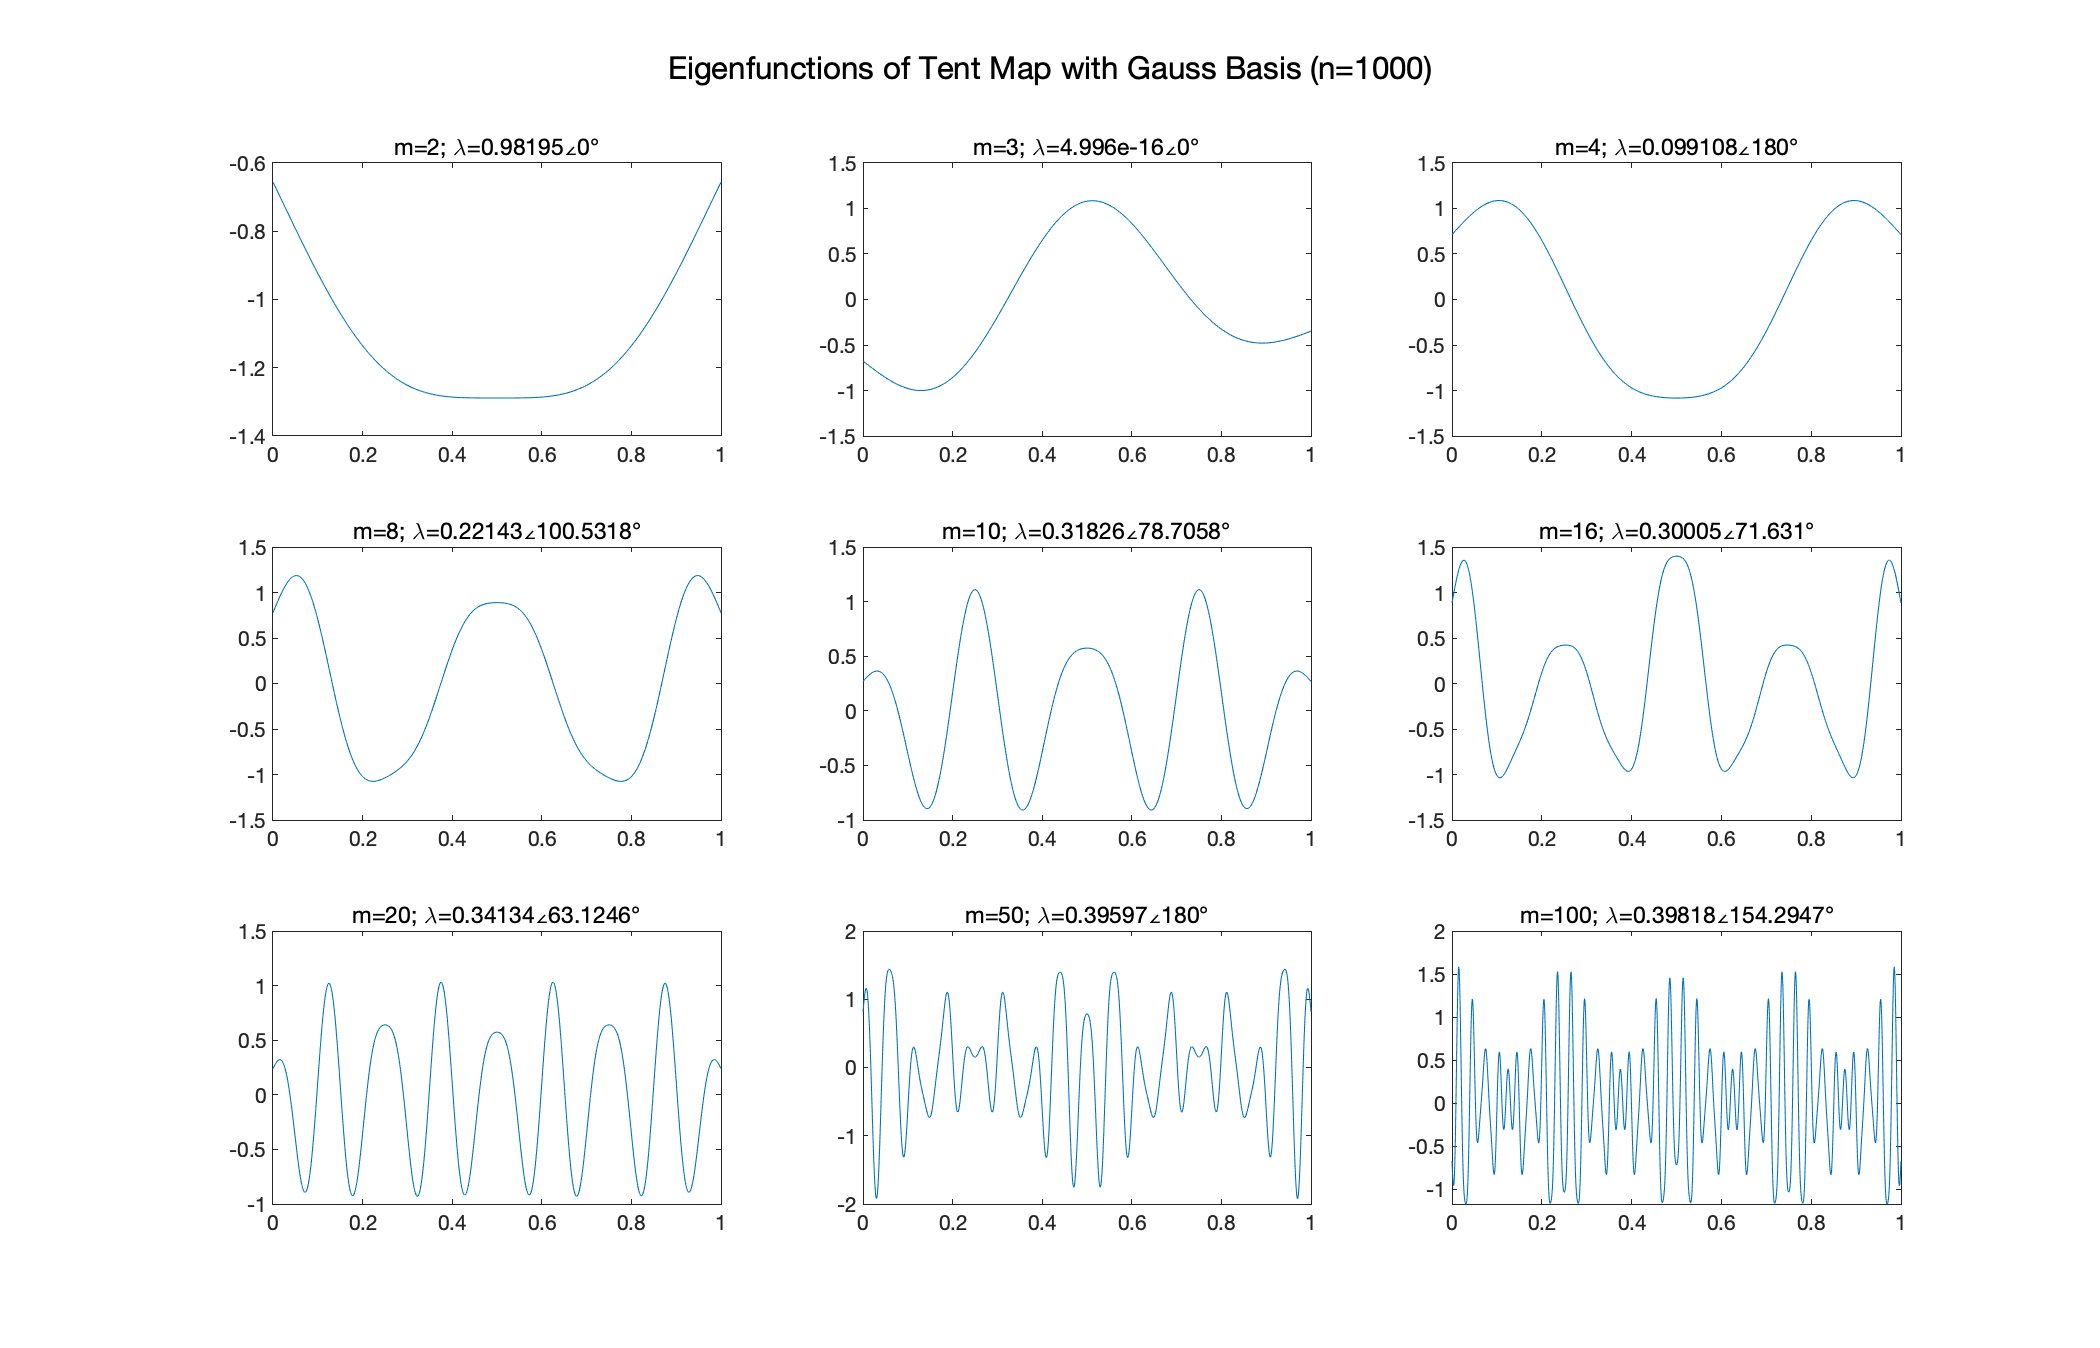
\includegraphics[scale=0.2]{tent/Tent_eigen_Gauss_n1000_m2-3-4-8-10-16-20-50-100}}
    \\
  \subfloat[傅里叶基函数]{
    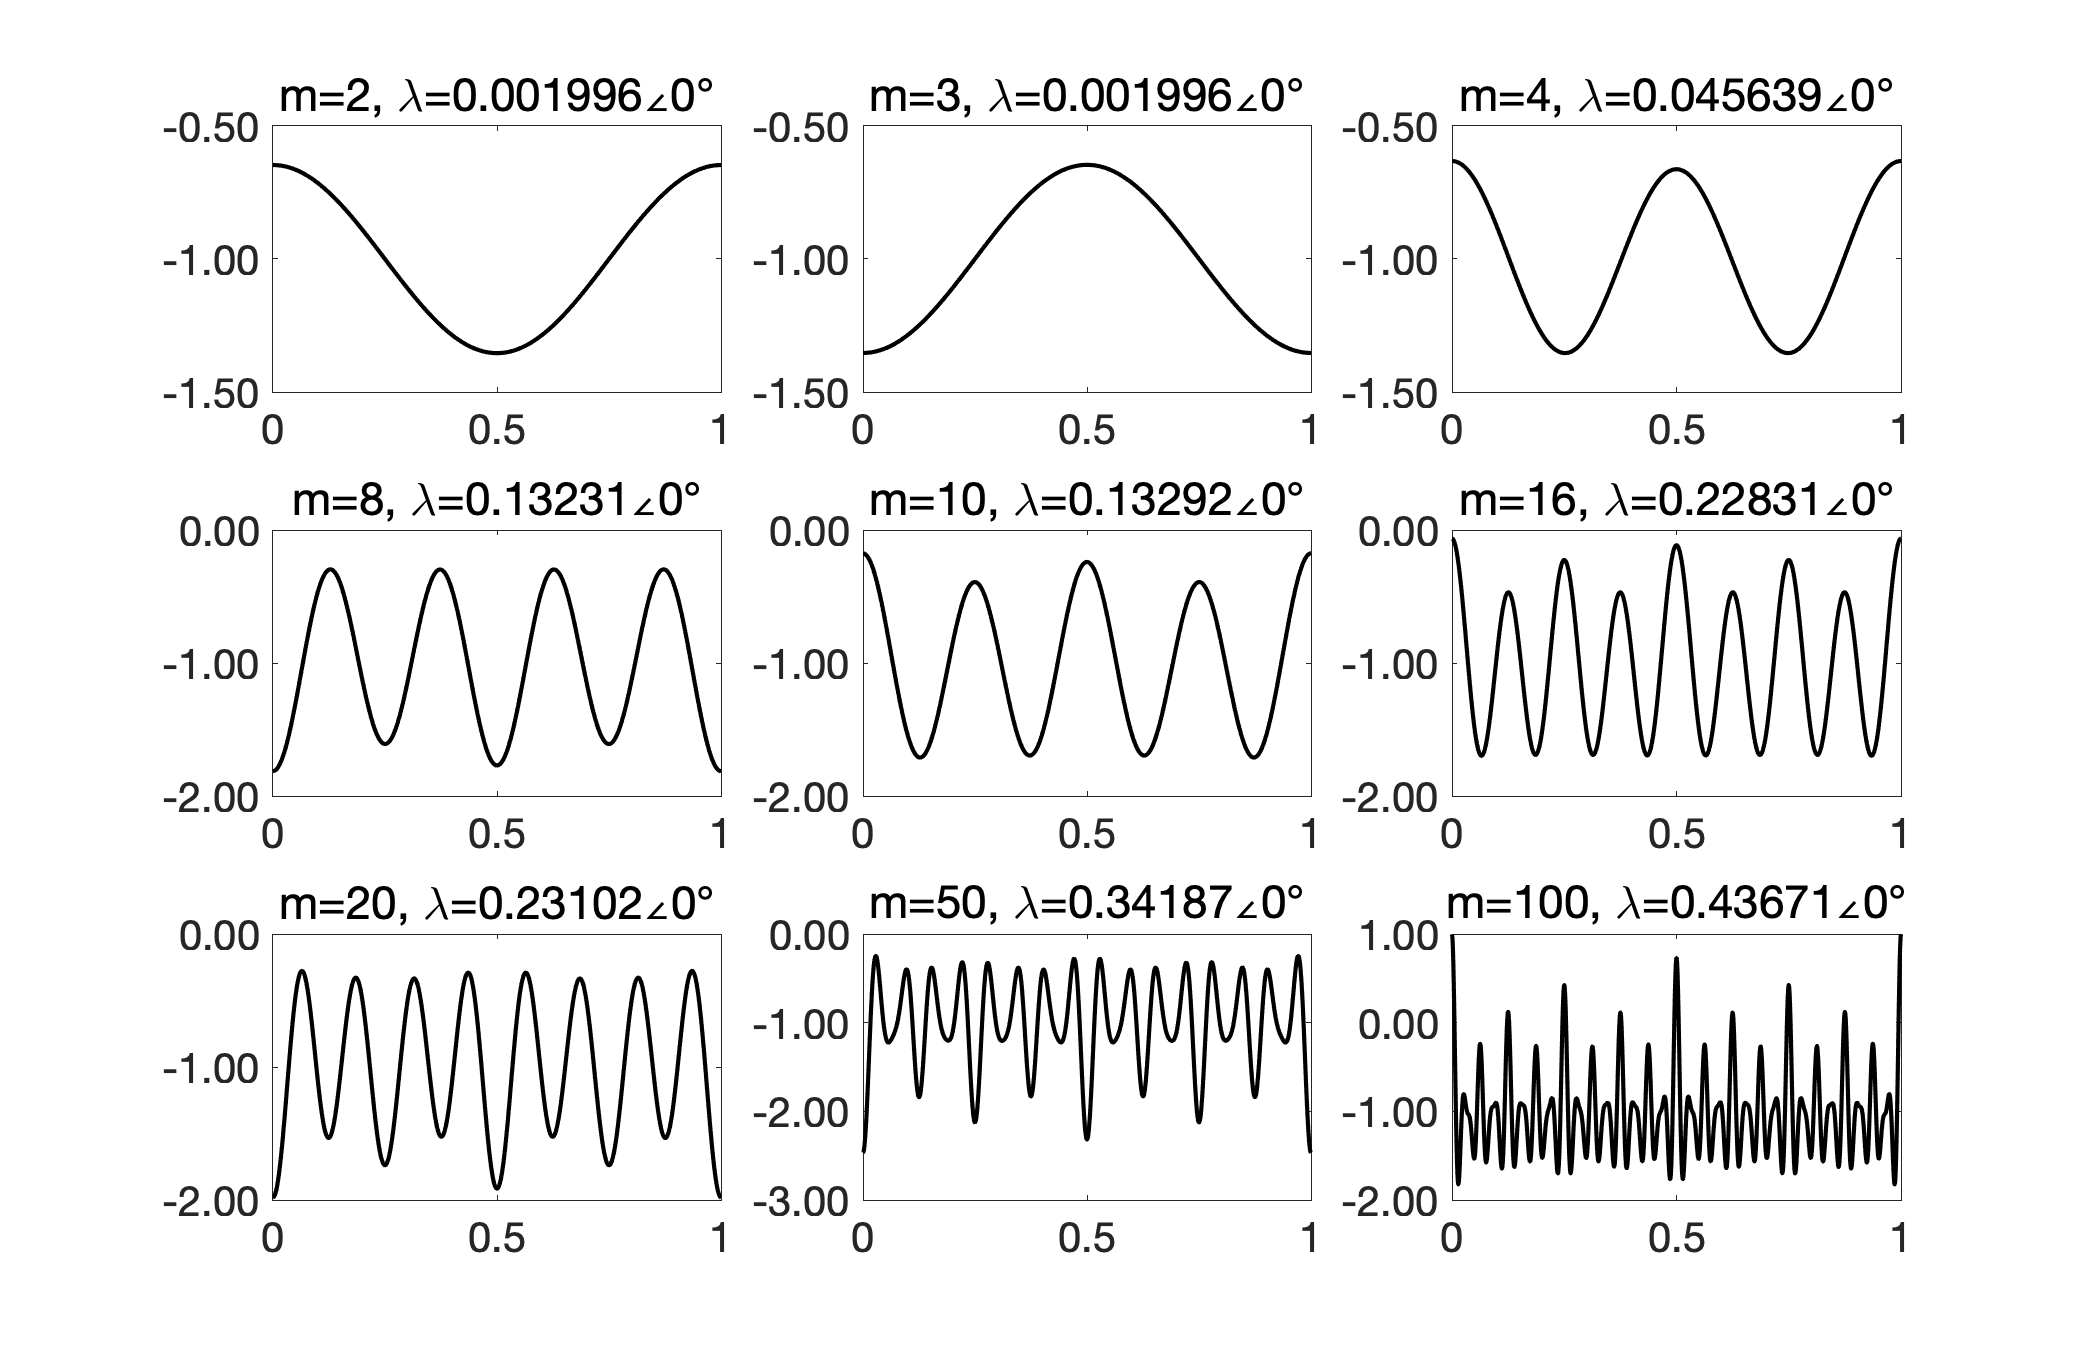
\includegraphics[scale=0.2]{tent/Tent_eigen_Fourier_n1000_m2-3-4-8-10-16-20-50-100}}
  \subfloat[勒让德基函数]{
    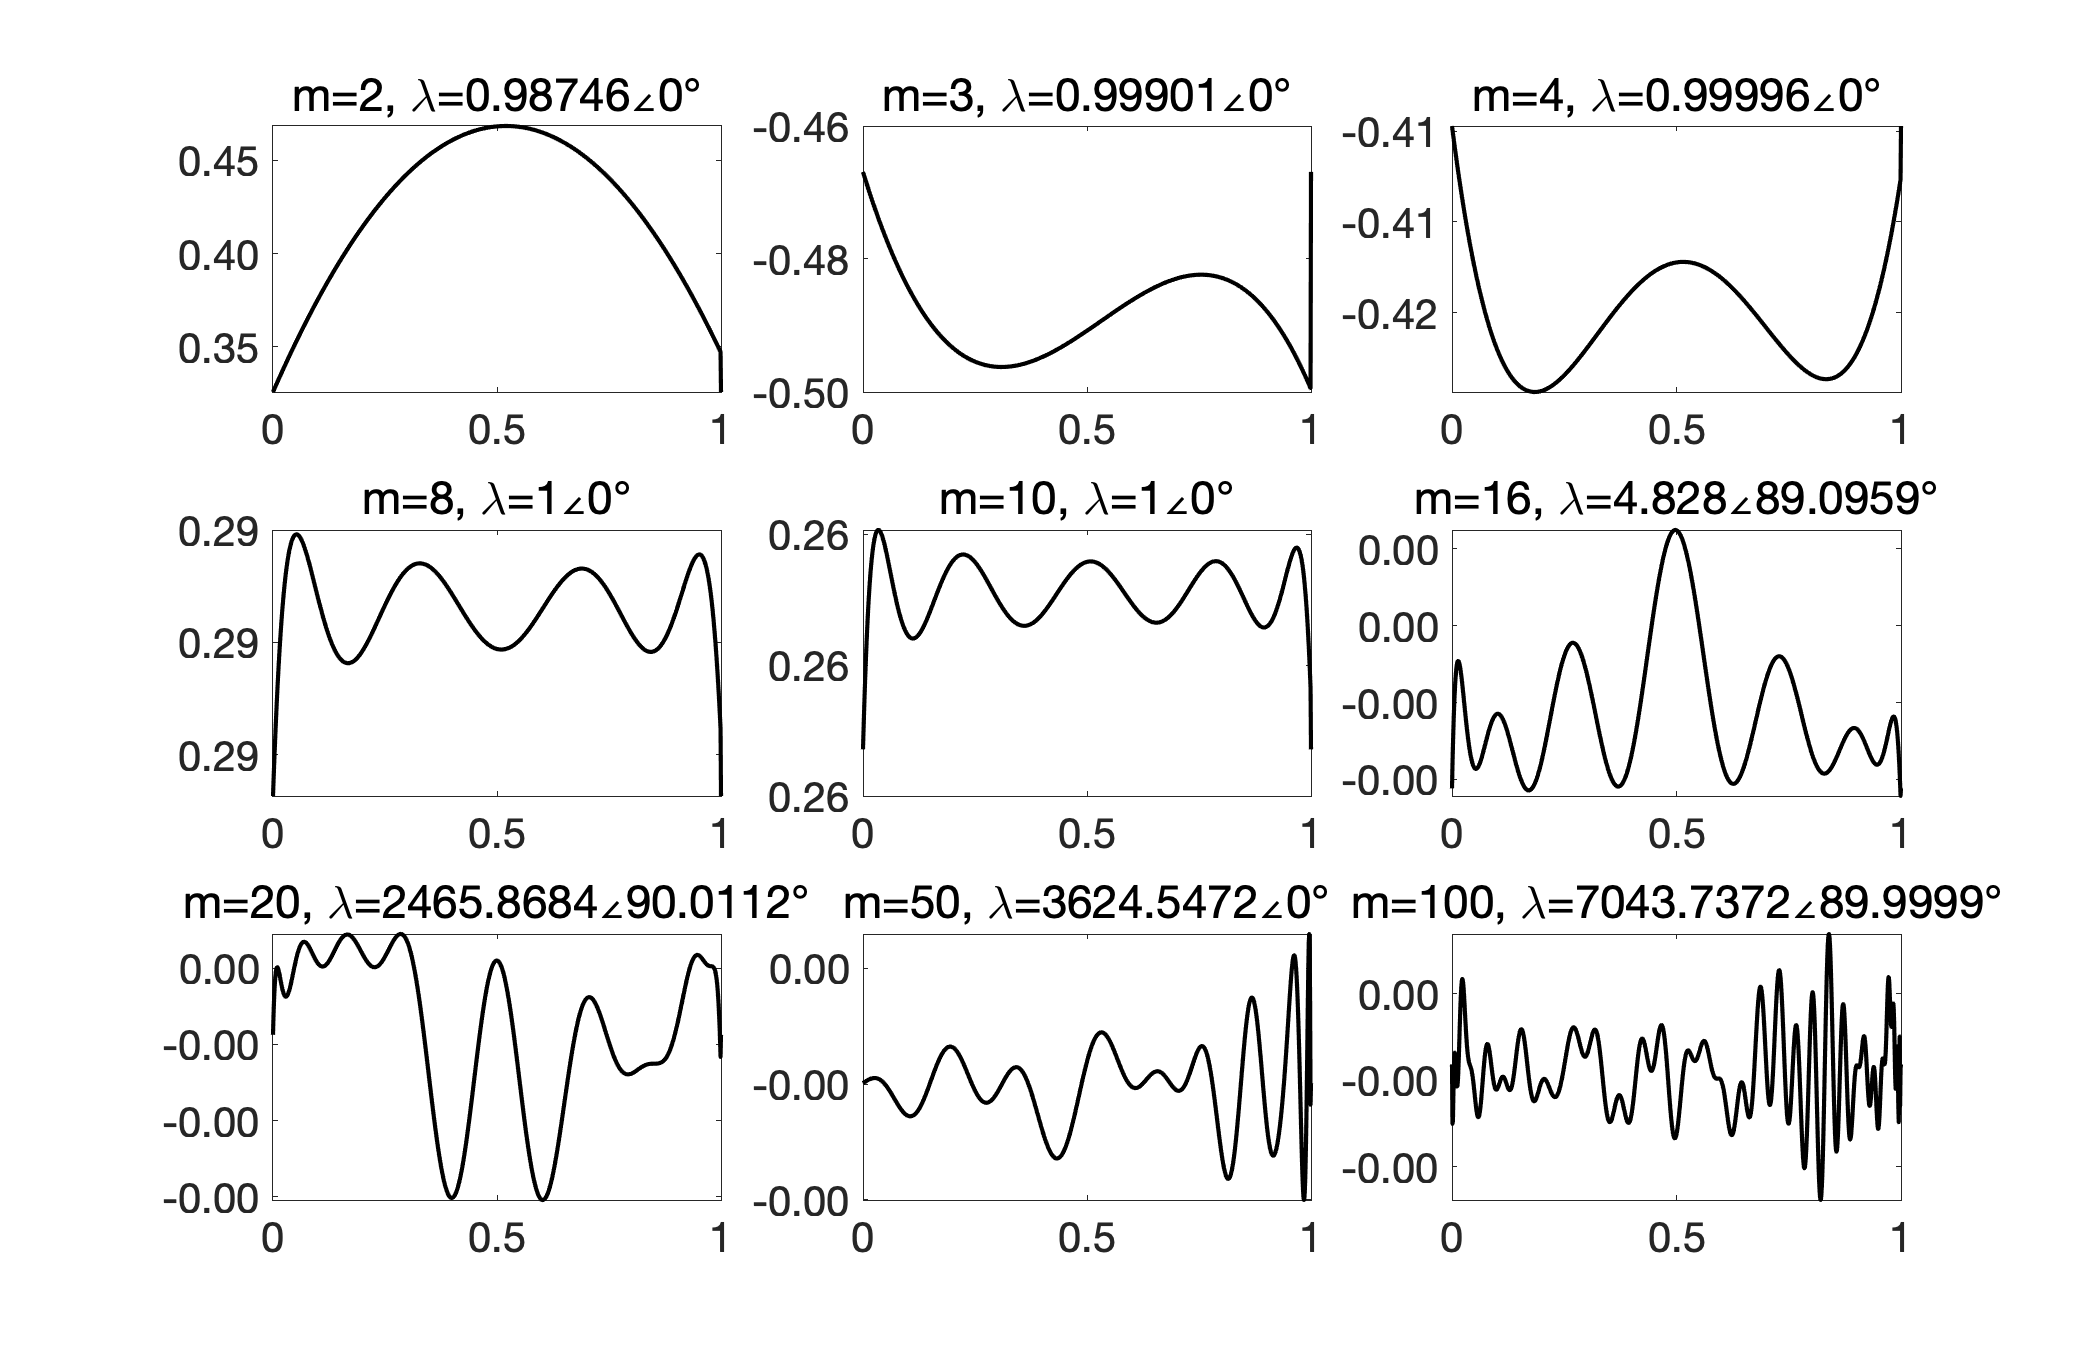
\includegraphics[scale=0.2]{tent/Tent_eigen_Legendre_n1000_m2-3-4-8-10-16-20-50-100}}
  \caption{不同基函数数量下帐篷映射的本征函数}
\end{figure}
\subsubsection{自然基函数空间}
\begin{figure}
	\centering
	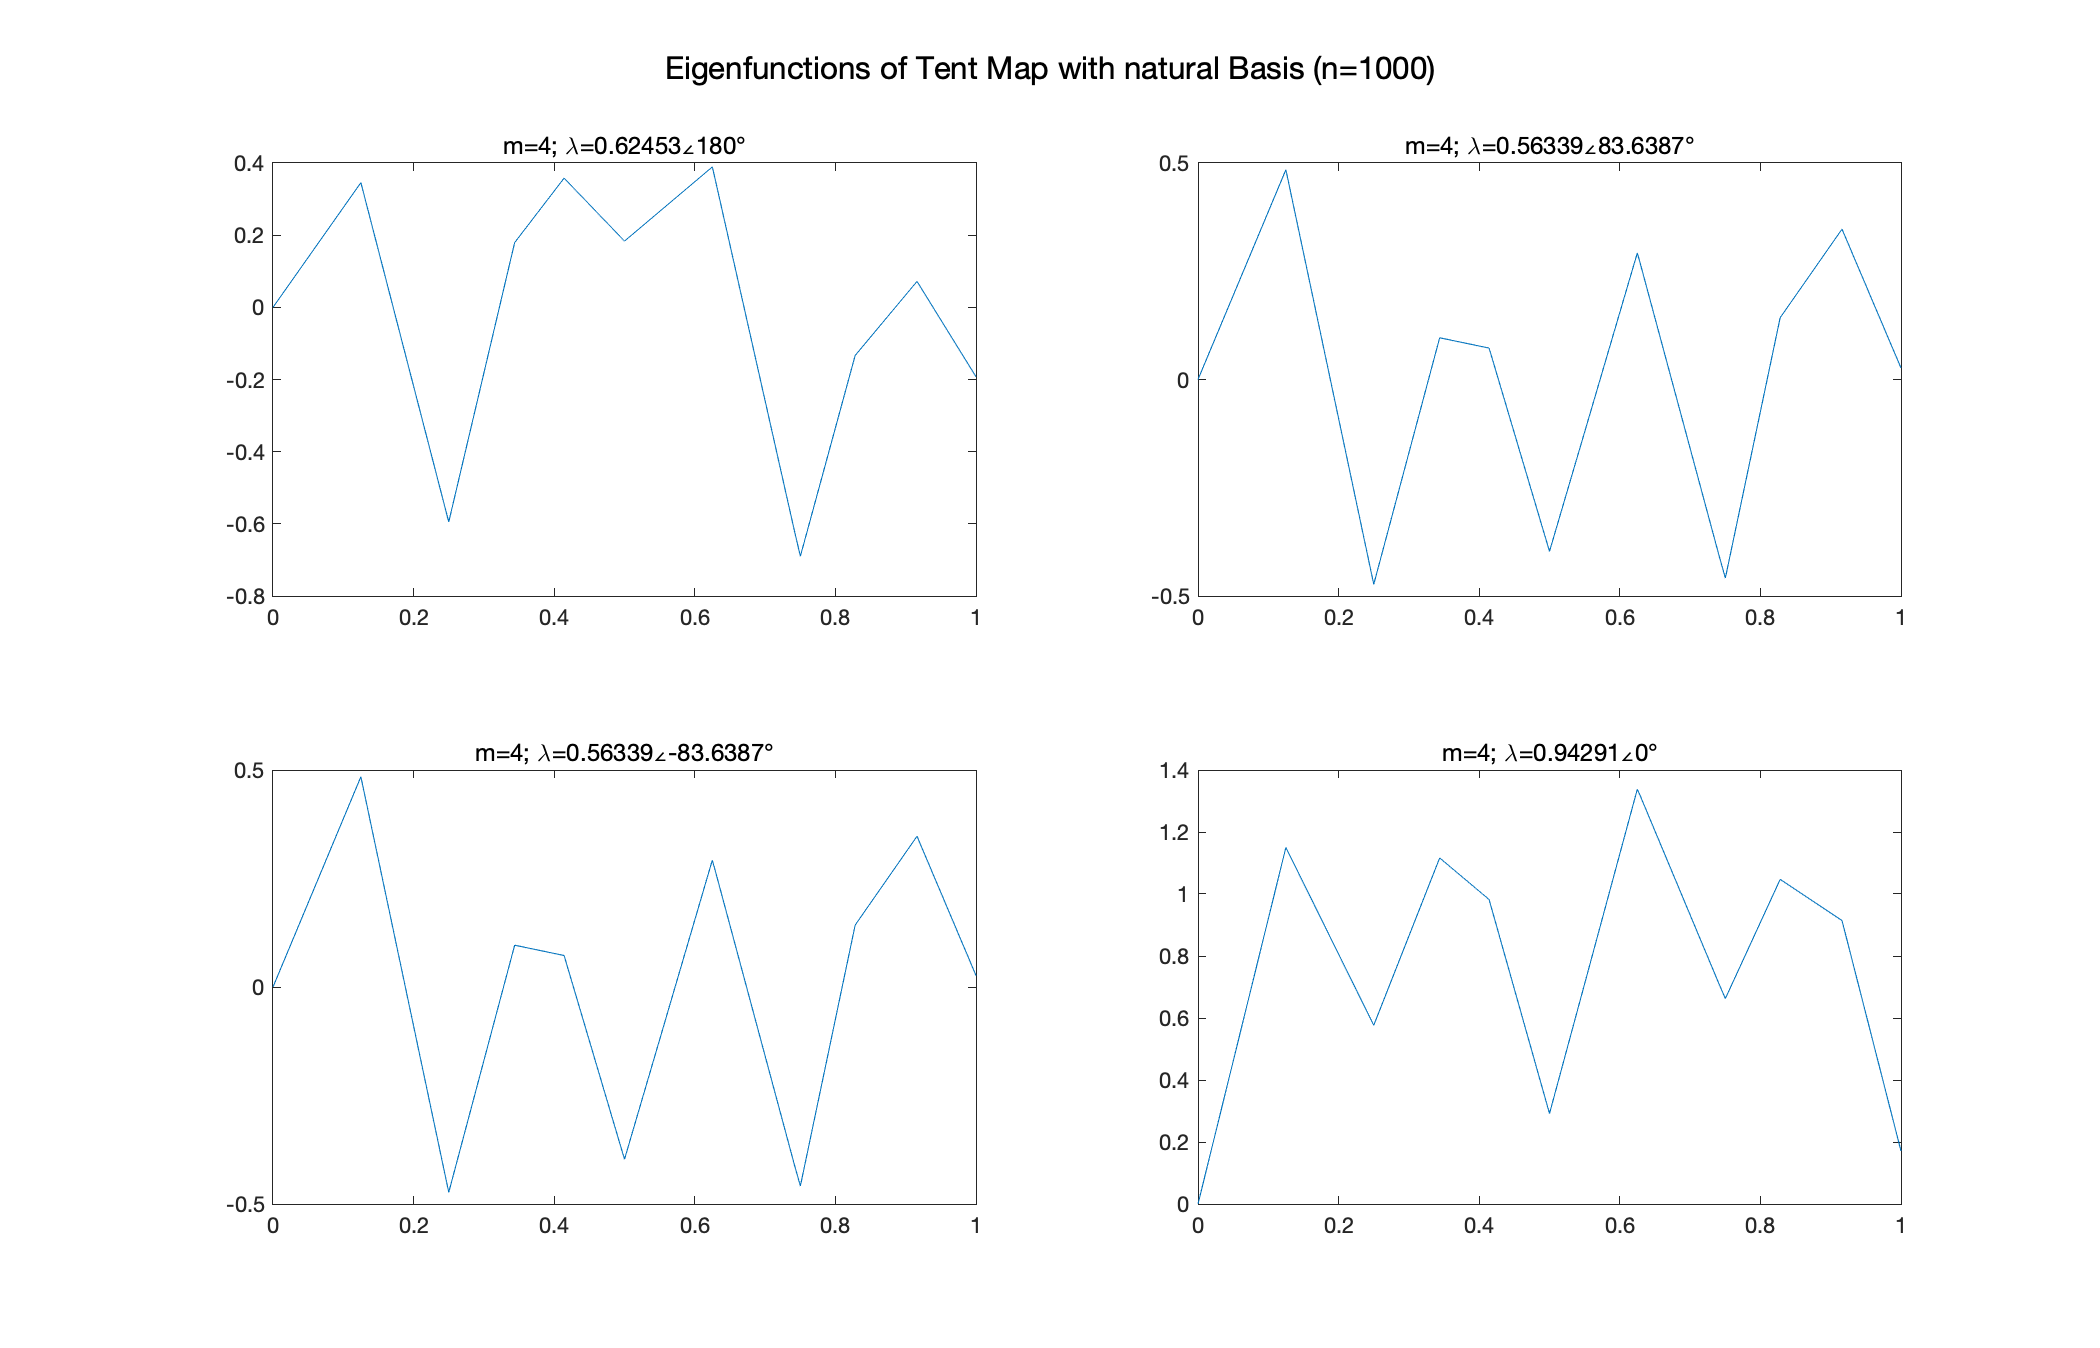
\includegraphics[scale=0.4]{tent/Tent_eigen_natural_n1000_m4}
    \caption{自然基函数下帐篷映射的本征函数($m=4$)}
\end{figure}
\begin{figure}
	\centering
	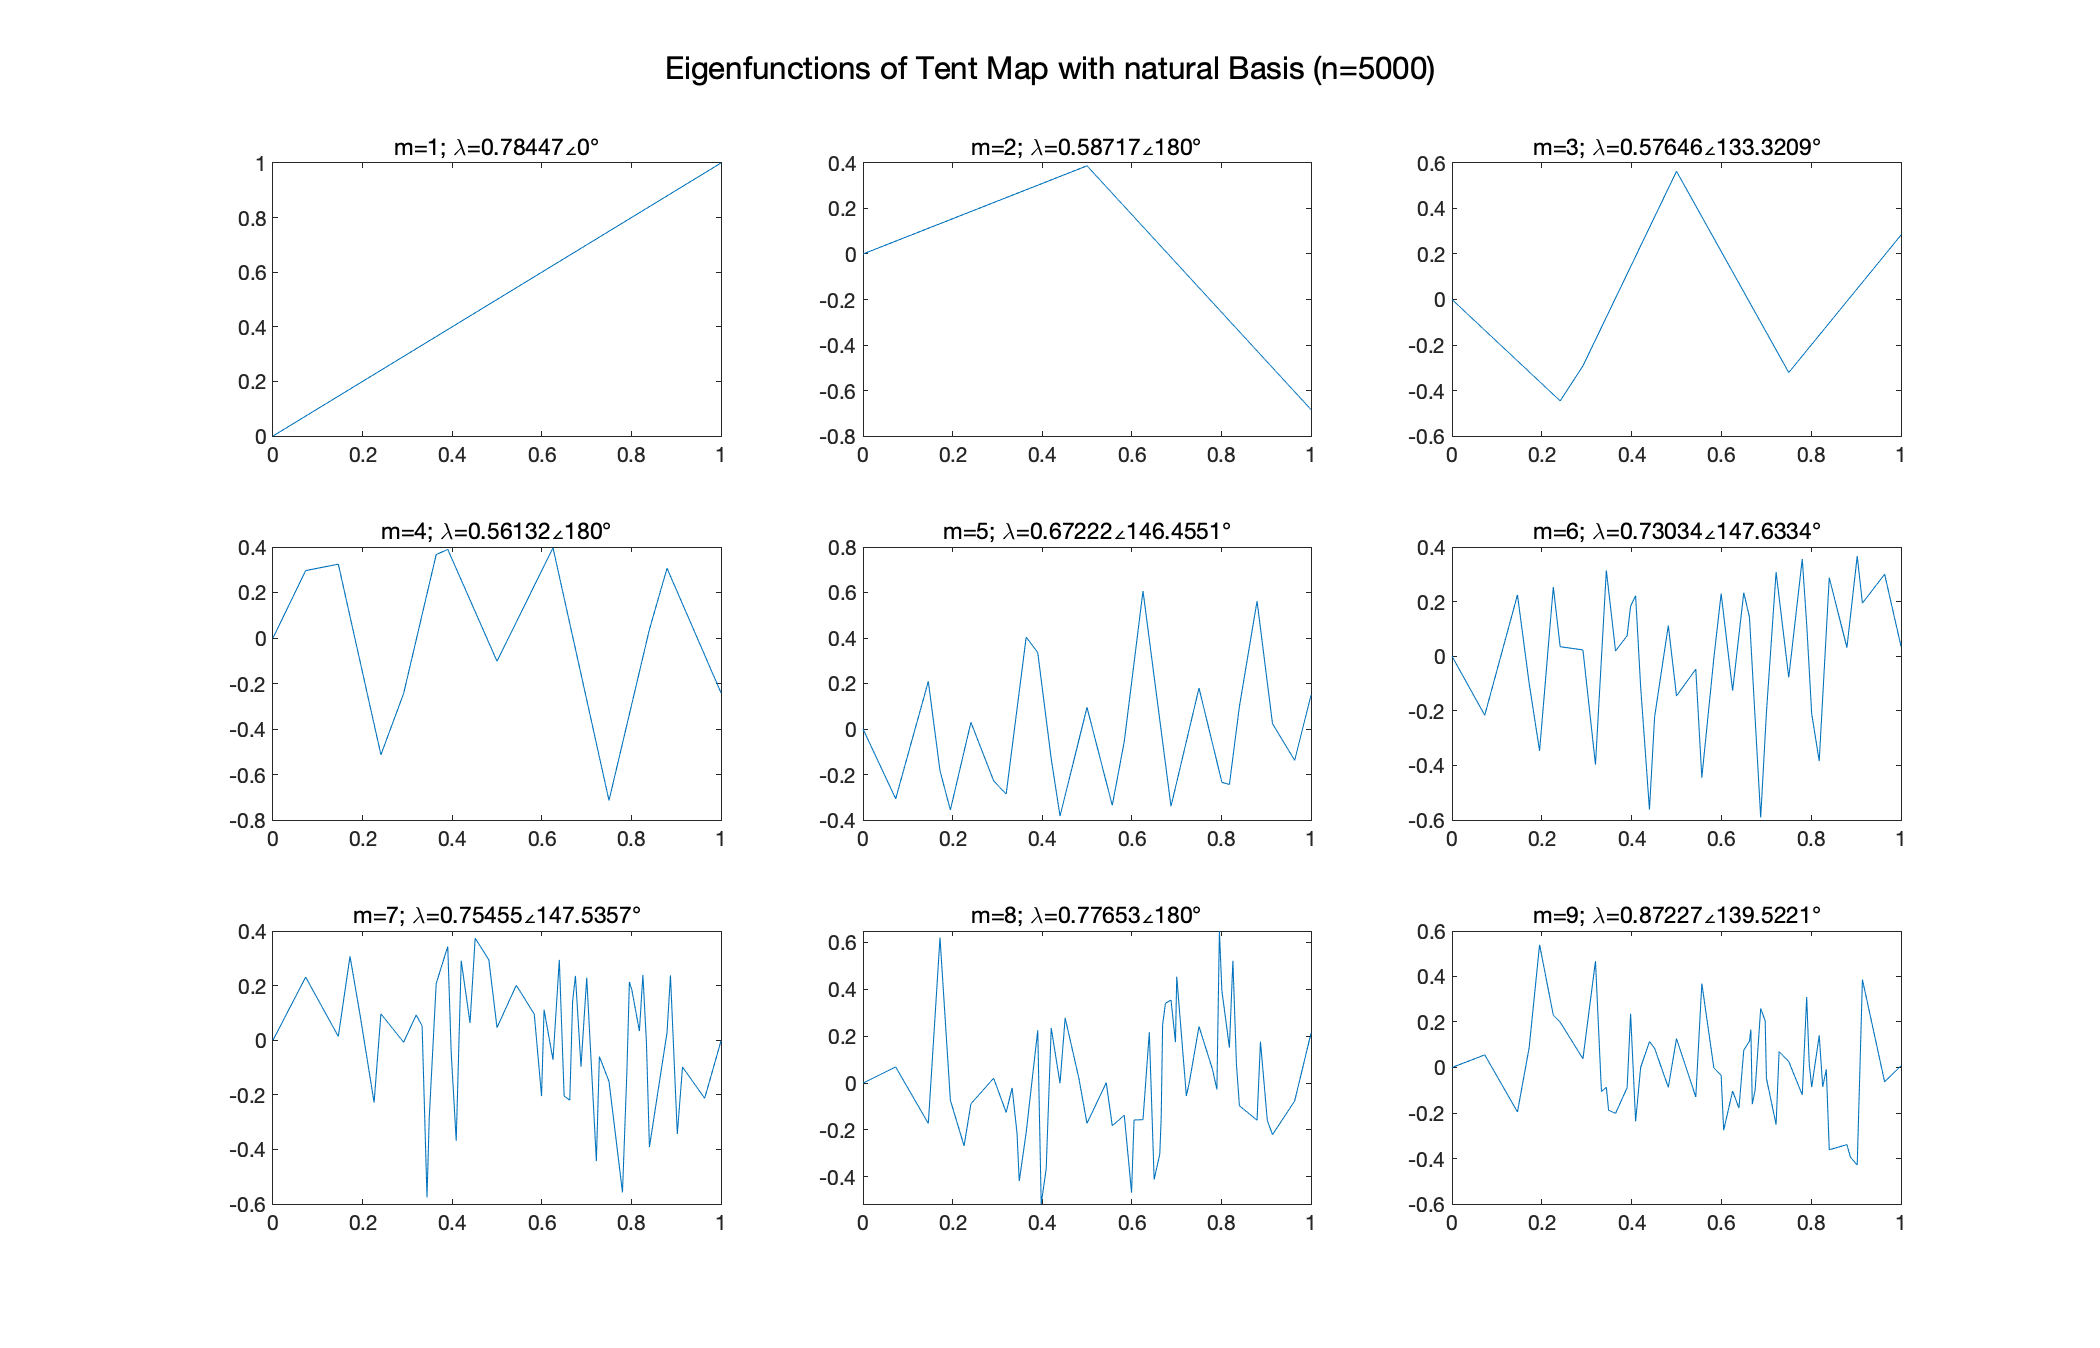
\includegraphics[scale=0.4]{tent/Tent_eigen_natural_n5000_m1-2-3-4-5-6-7-8-9}
    \caption{不同基函数数量下帐篷映射的本征函数}
\end{figure}

\subsection{Koopman算符对帐篷映射的相空间划分}
\begin{table}[]
  \centering
  \begin{tabular}{|c|c|}
  \hline
  迭代次数 & 边界点($x=0$) \\ \hline
  1 & 0,\textbf{\underline{1}} \\ \hline
  2 & 0,\textbf{\underline{0.5}},1 \\ \hline
  3 & 0,\textbf{\underline{0.25}},0.5,\textbf{\underline{0.75}},1 \\ \hline
  4 & 0,\textbf{\underline{0.125}},0.25,\textbf{\underline{0.375}},0.5,\textbf{\underline{0.625}},0.75,\textbf{\underline{0.875}},1 \\ \hline
  5 & 0,\textbf{\underline{0.0625}},0.125,\textbf{\underline{0.1875}},0.25,\textbf{\underline{0.3125}},0.375,\textbf{\underline{0.4375}},0.5,\textbf{\underline{0.5625}},0.625,\textbf{\underline{0.6875}},0.75,\textbf{\underline{0.8125}},0.875,\textbf{\underline{0.9375}},1 \\ \hline
  \end{tabular}
  \caption{帐篷映射的边界点($x=0$)}
\end{table}
\begin{figure}
	\centering
	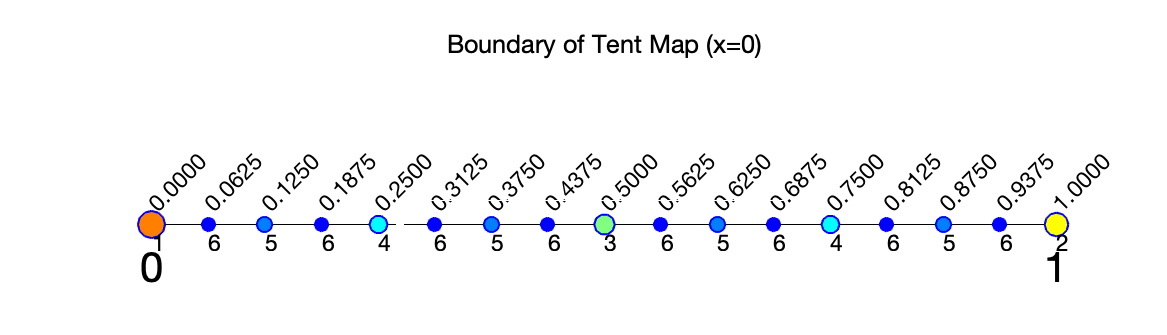
\includegraphics[scale=0.8]{tent/Tent_boundarys_x0}
    \caption{帐篷映射的边界点($x=0$)}
\end{figure}
\begin{table}[]
  \centering
  \begin{tabular}{|c|c|}
  \hline
  迭代次数 & 边界点($x=\frac{2}{3}$) \\ \hline
  0 & 0.6666 \\ \hline
  1 & \textbf{\underline{0.3333}},0.6666 \\ \hline
  2 & \textbf{\underline{0.1666}},0.3333,0.6666,\textbf{\underline{0.8333}} \\ \hline
  3 & \textbf{\underline{0.0833}},0.1666,0.3333,\textbf{\underline{0.4166}},\textbf{\underline{0.5833}},0.6666,0.8333,\textbf{\underline{0.9166}} \\ \hline
  4 & \begin{tabular}[c]{@{}l@{}}\textbf{\underline{0.04166}},0.0833,0.1666,\textbf{\underline{0.2083}},\textbf{\underline{0.2916}},0.3333,0.4166,\textbf{\underline{0.4583}},\\ \textbf{\underline{0.5416}},0.5833,0.6666,\textbf{\underline{0.7083}},\textbf{\underline{0.7916}},0.8333,0.9166,\textbf{\underline{0.9583}}\end{tabular} \\ \hline
  \end{tabular}
  \caption{帐篷映射的边界点($x=\frac{2}{3}$)}
\end{table}
\begin{figure}
	\centering
	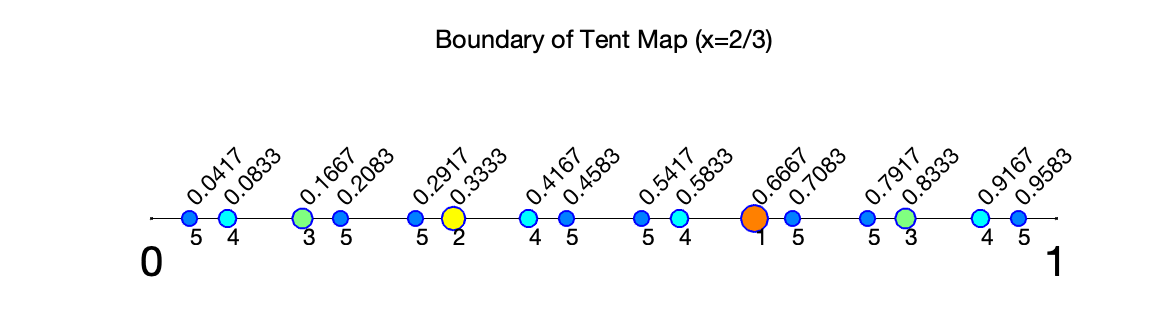
\includegraphics[scale=0.8]{tent/Tent_boundarys_x2-3}
    \caption{帐篷映射的边界点($x=\frac{2}{3}$)}
\end{figure}

\begin{figure}
  \centering%[2,3,4,5,8,10,15,20]
  \subfloat[m=2]{
    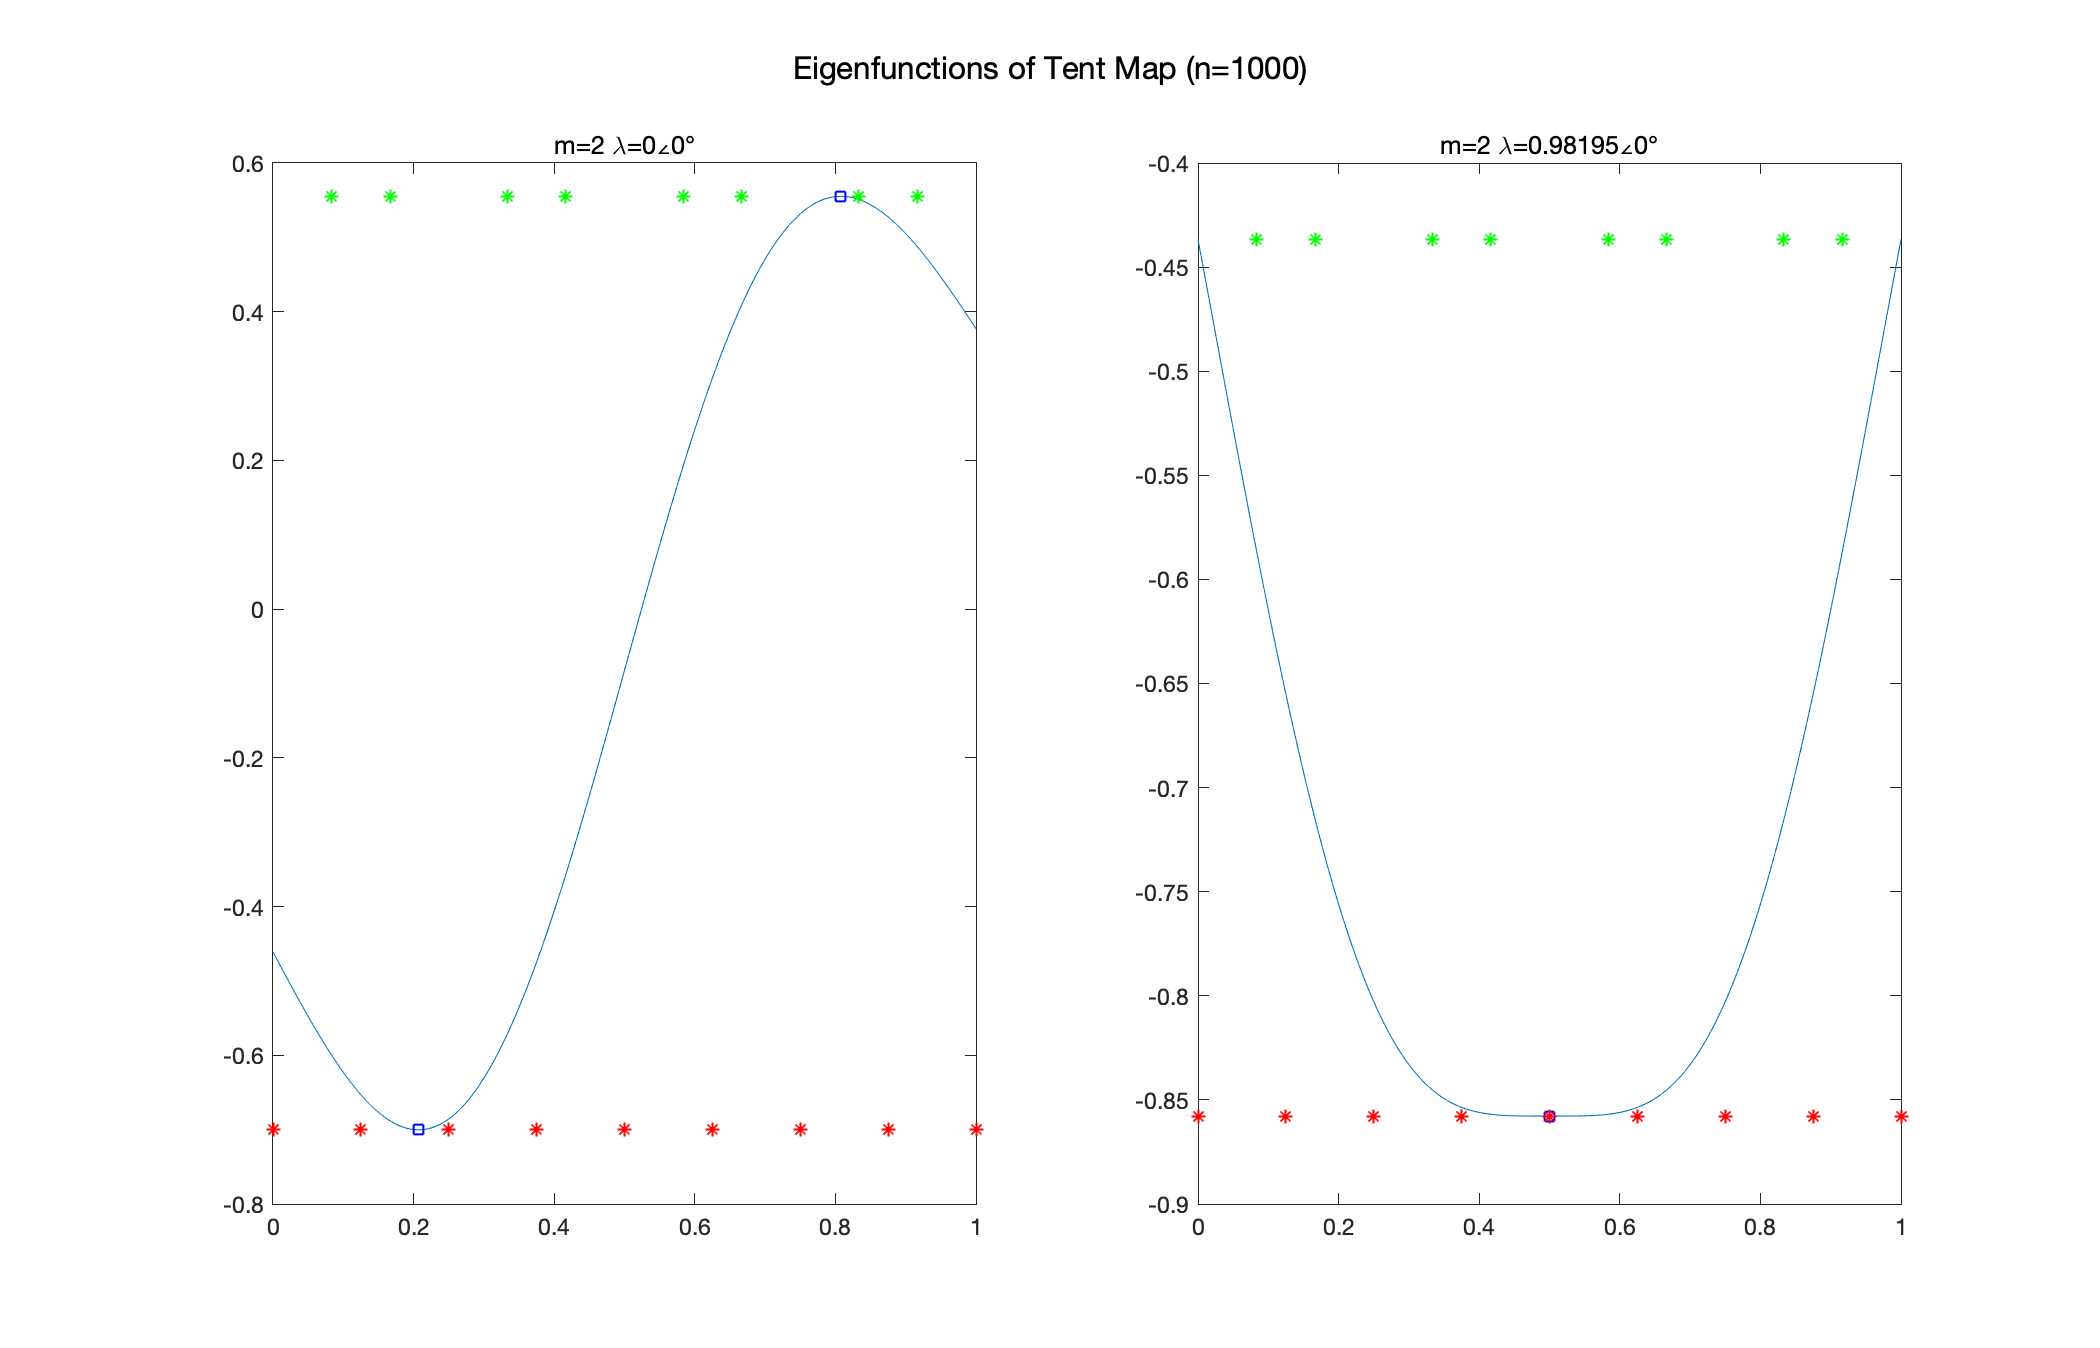
\includegraphics[scale=0.2]{tent/noise/Tent_eigen_noise_n1000m2d0}}
  \subfloat[m=3]{
    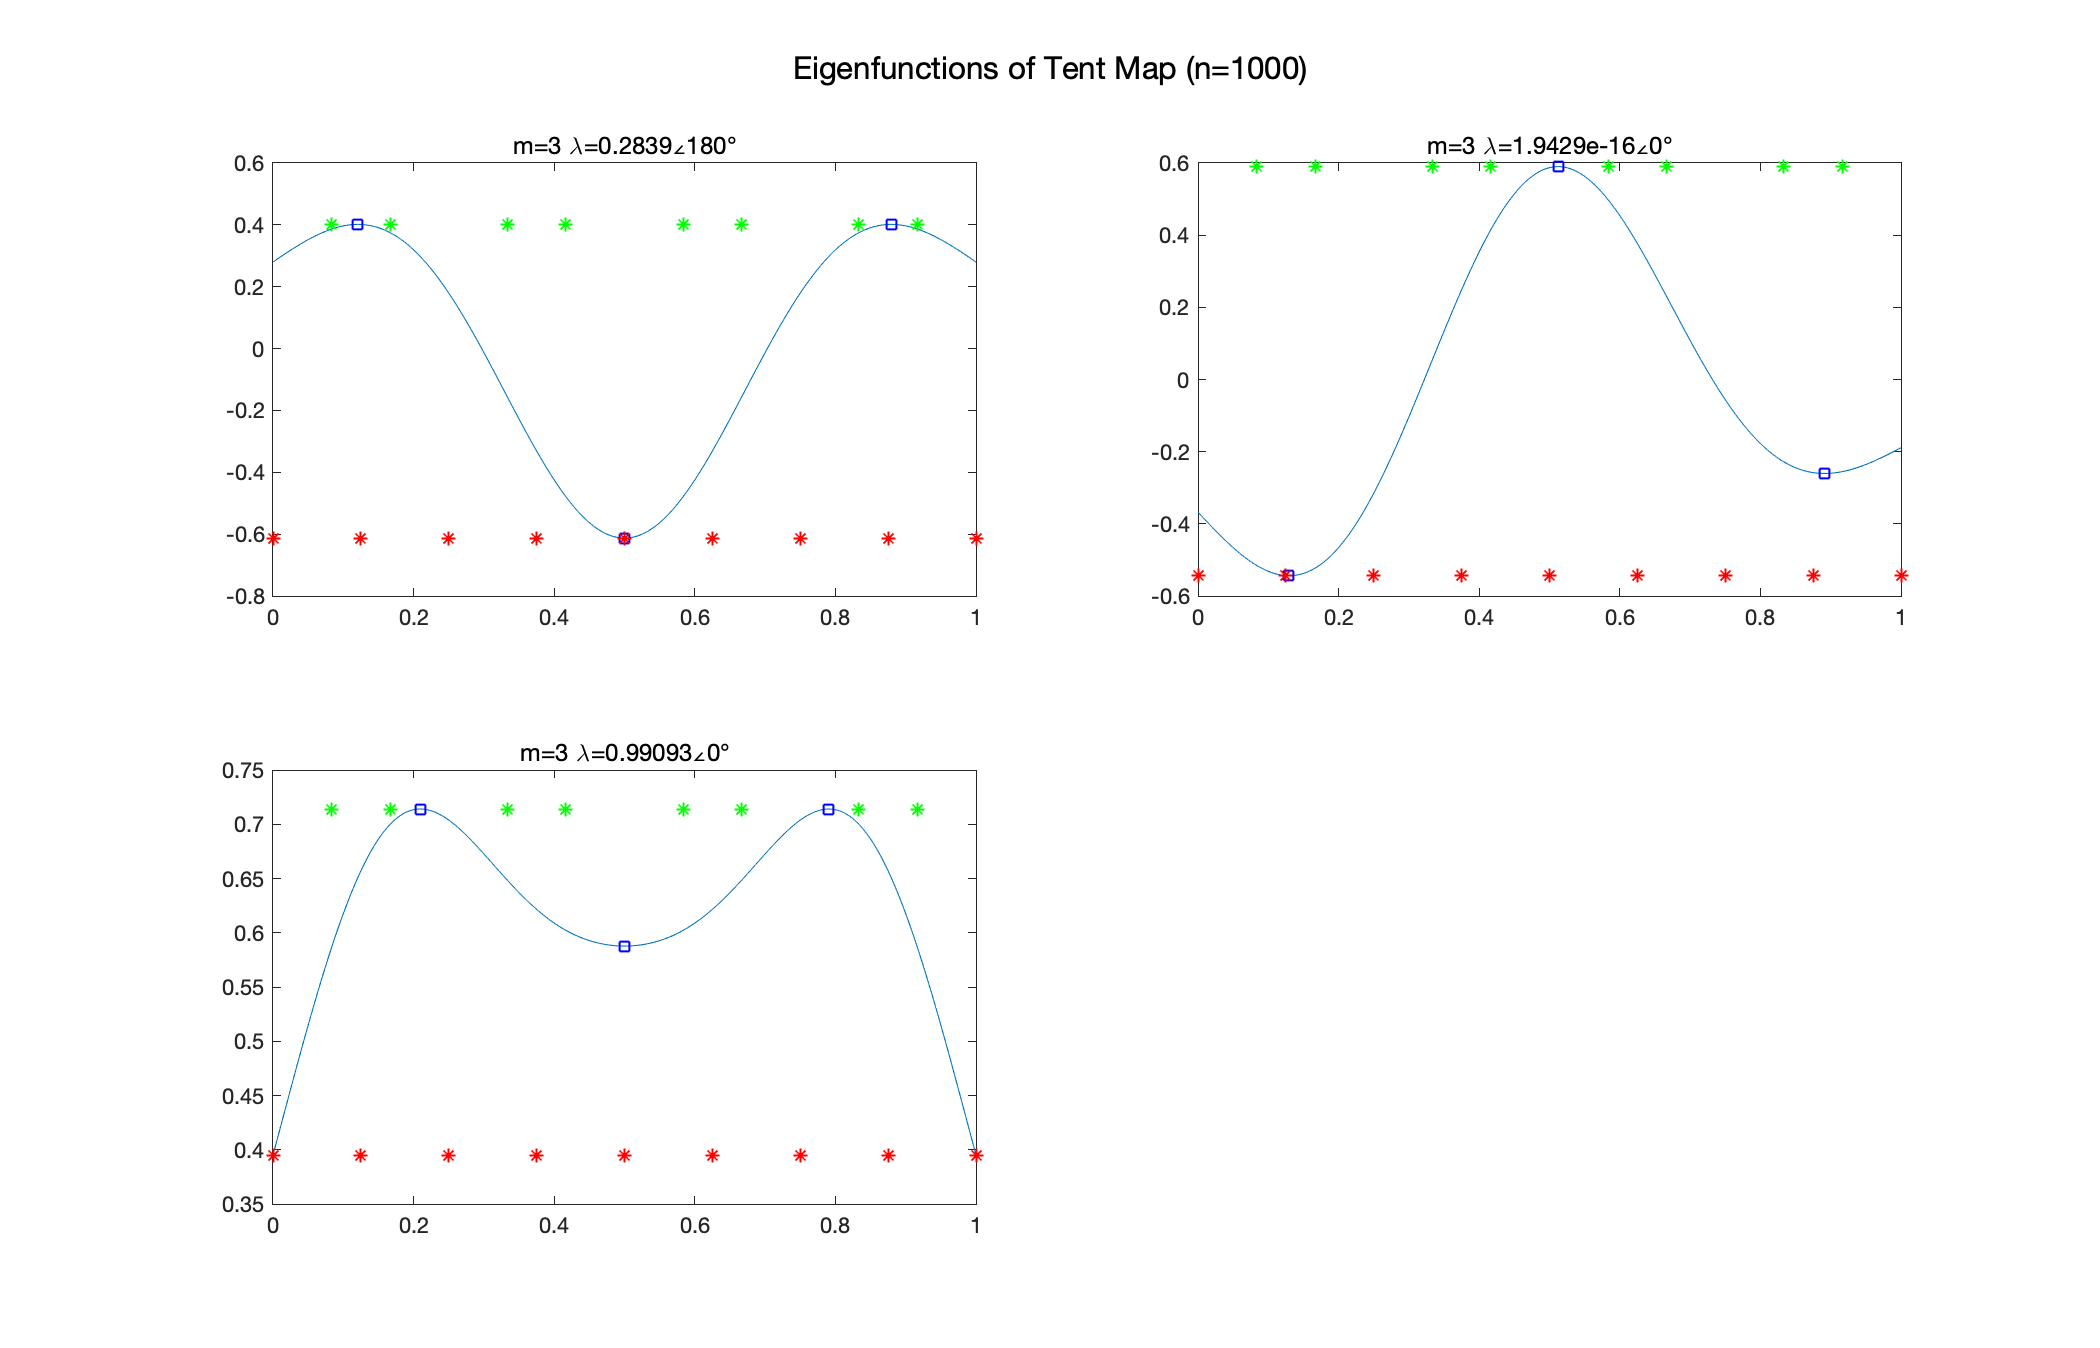
\includegraphics[scale=0.2]{tent/noise/Tent_eigen_noise_n1000m3d0}}
    \\
  \subfloat[m=4]{
    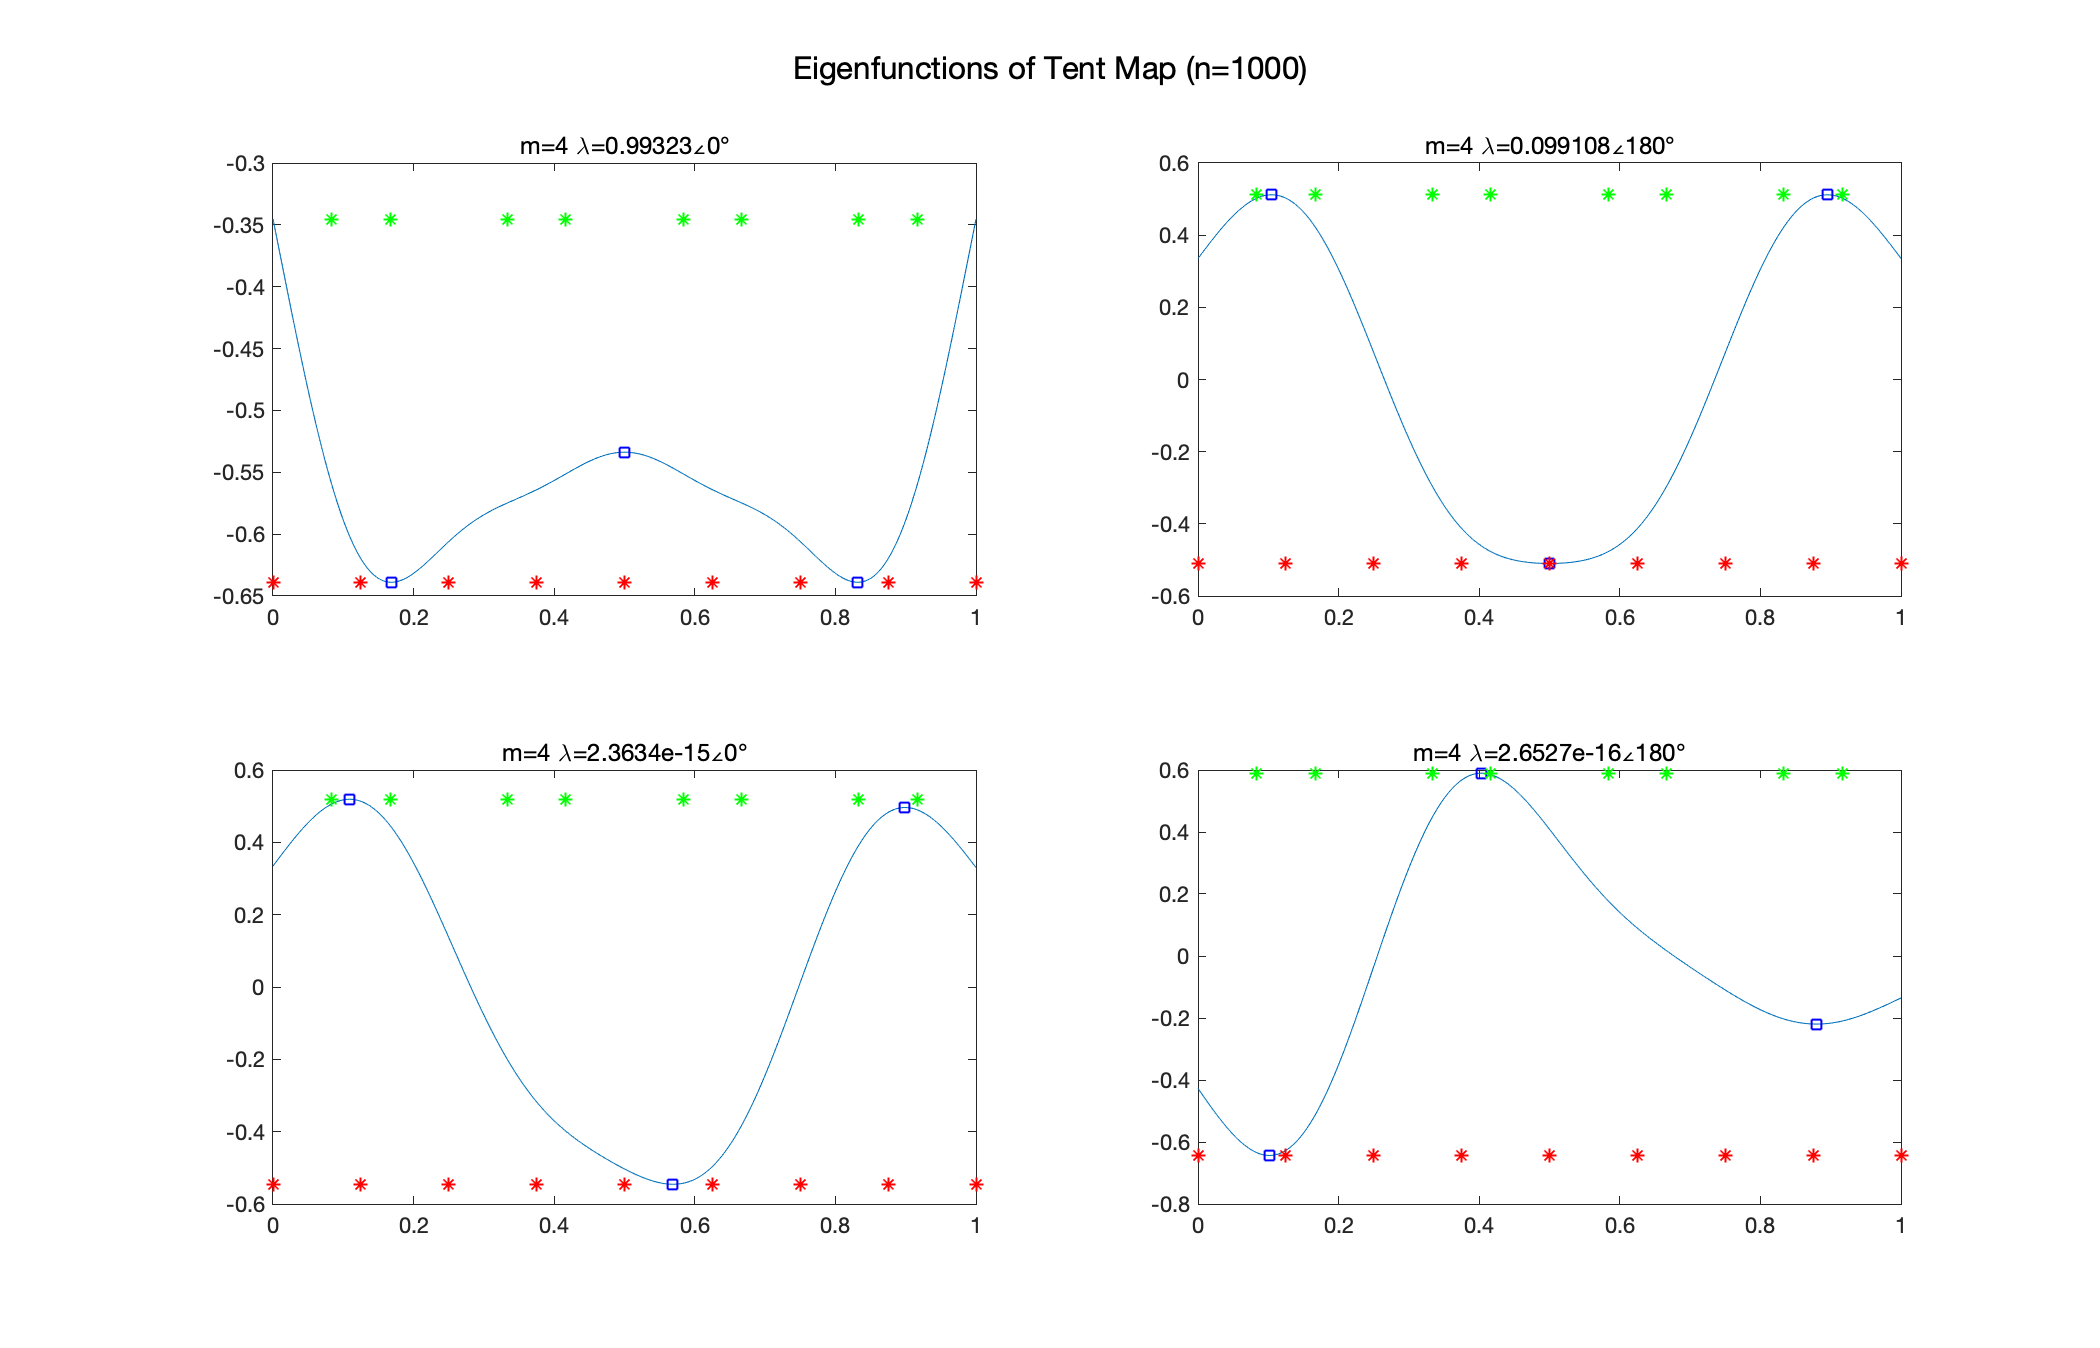
\includegraphics[scale=0.2]{tent/noise/Tent_eigen_noise_n1000m4d0}}
  \subfloat[m=5]{
    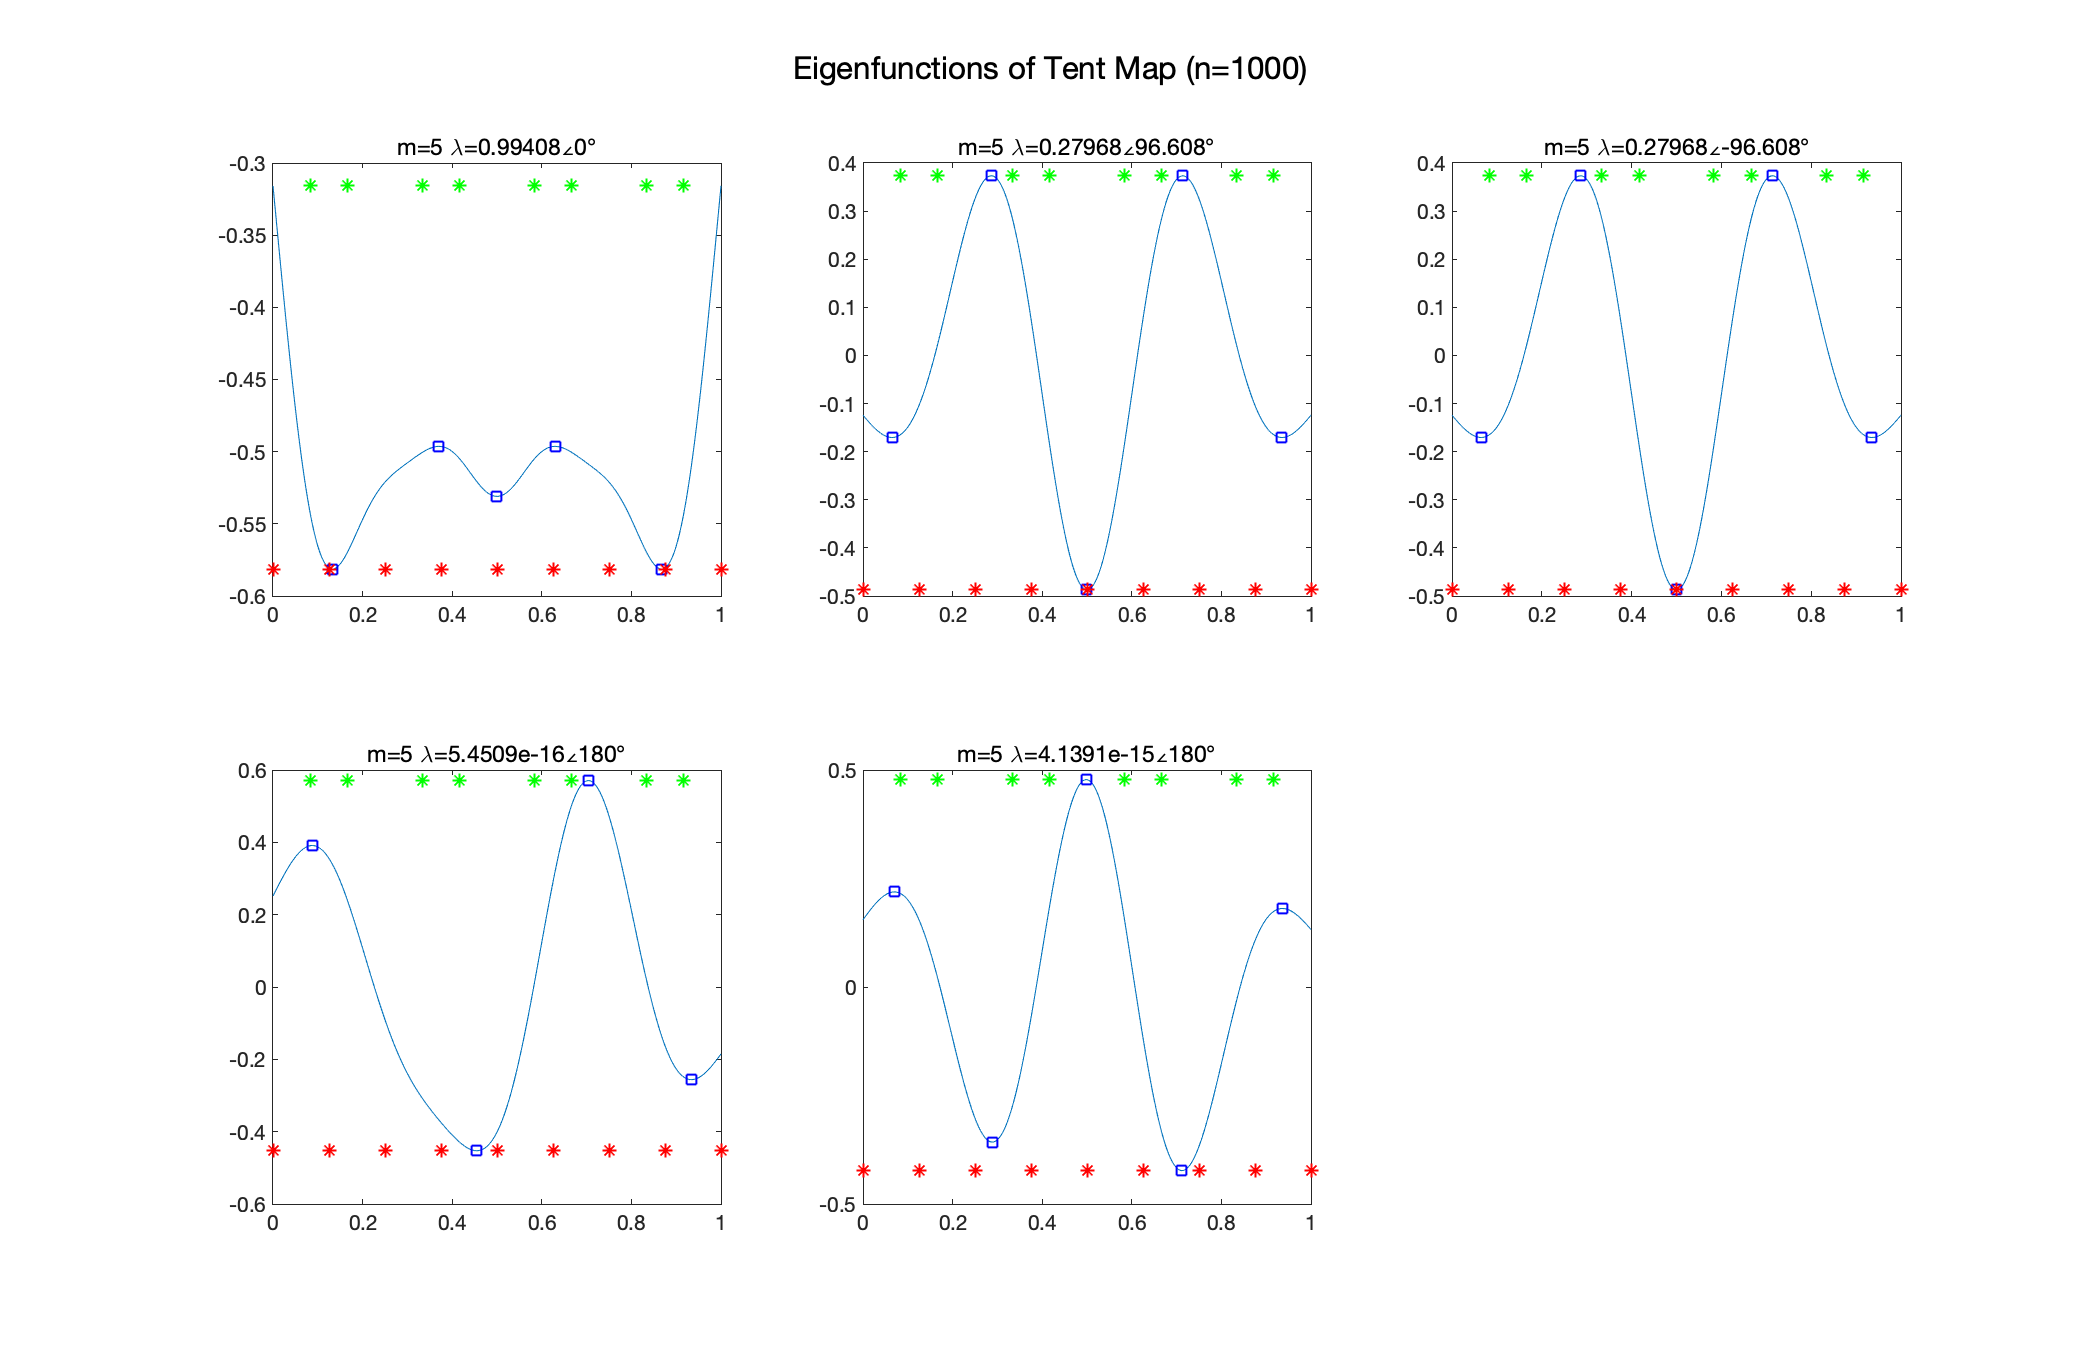
\includegraphics[scale=0.2]{tent/noise/Tent_eigen_noise_n1000m5d0}}
    \\
  \subfloat[m=8]{
    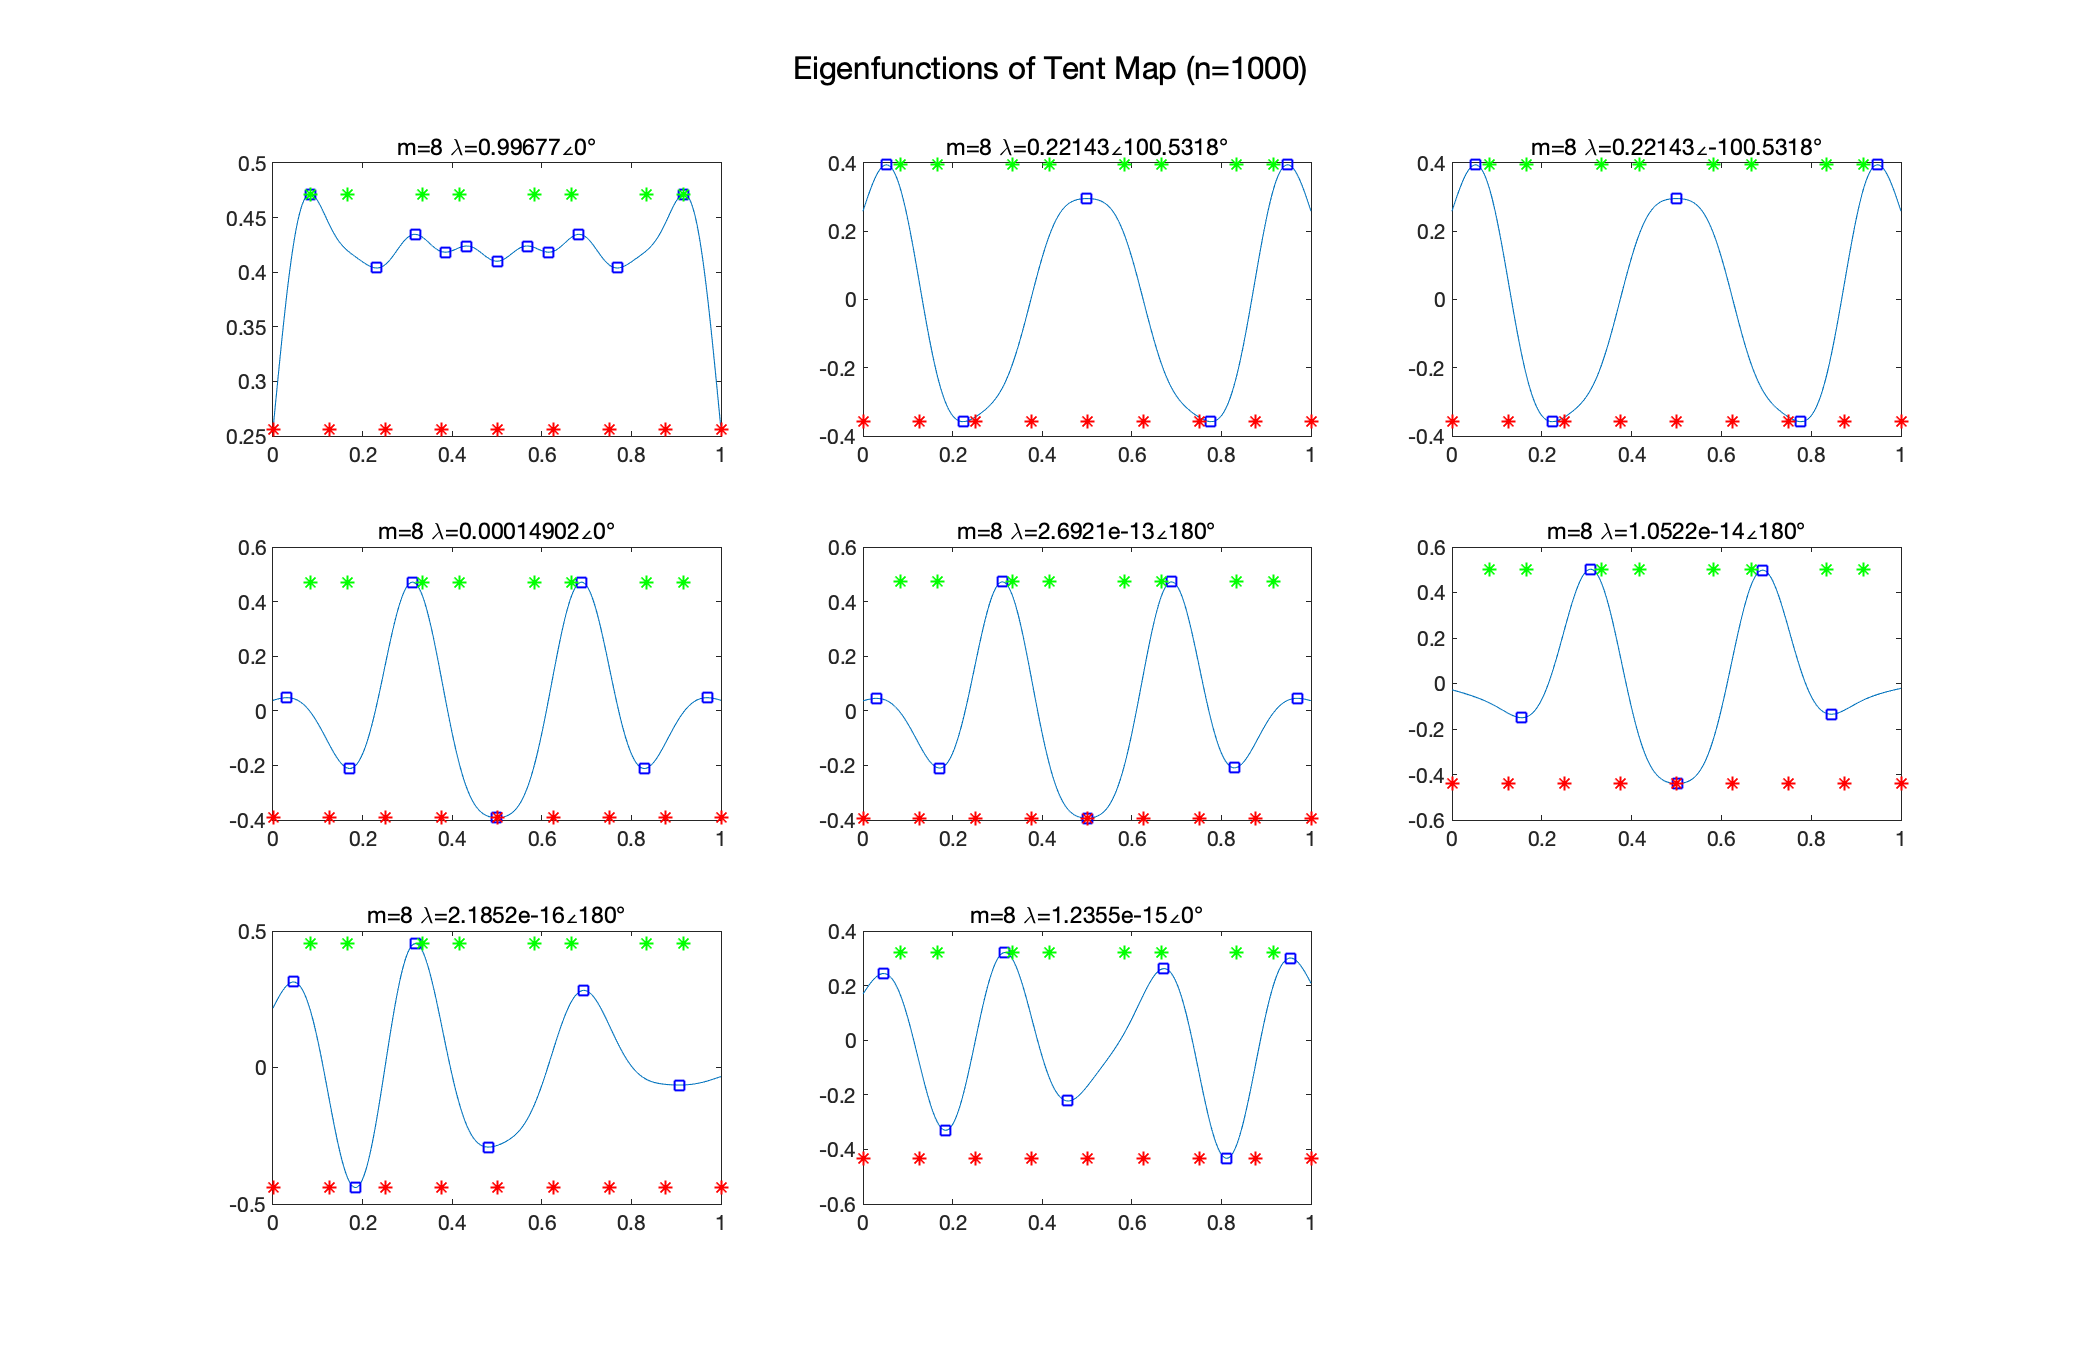
\includegraphics[scale=0.2]{tent/noise/Tent_eigen_noise_n1000m8d0}}
  \subfloat[m=10]{
    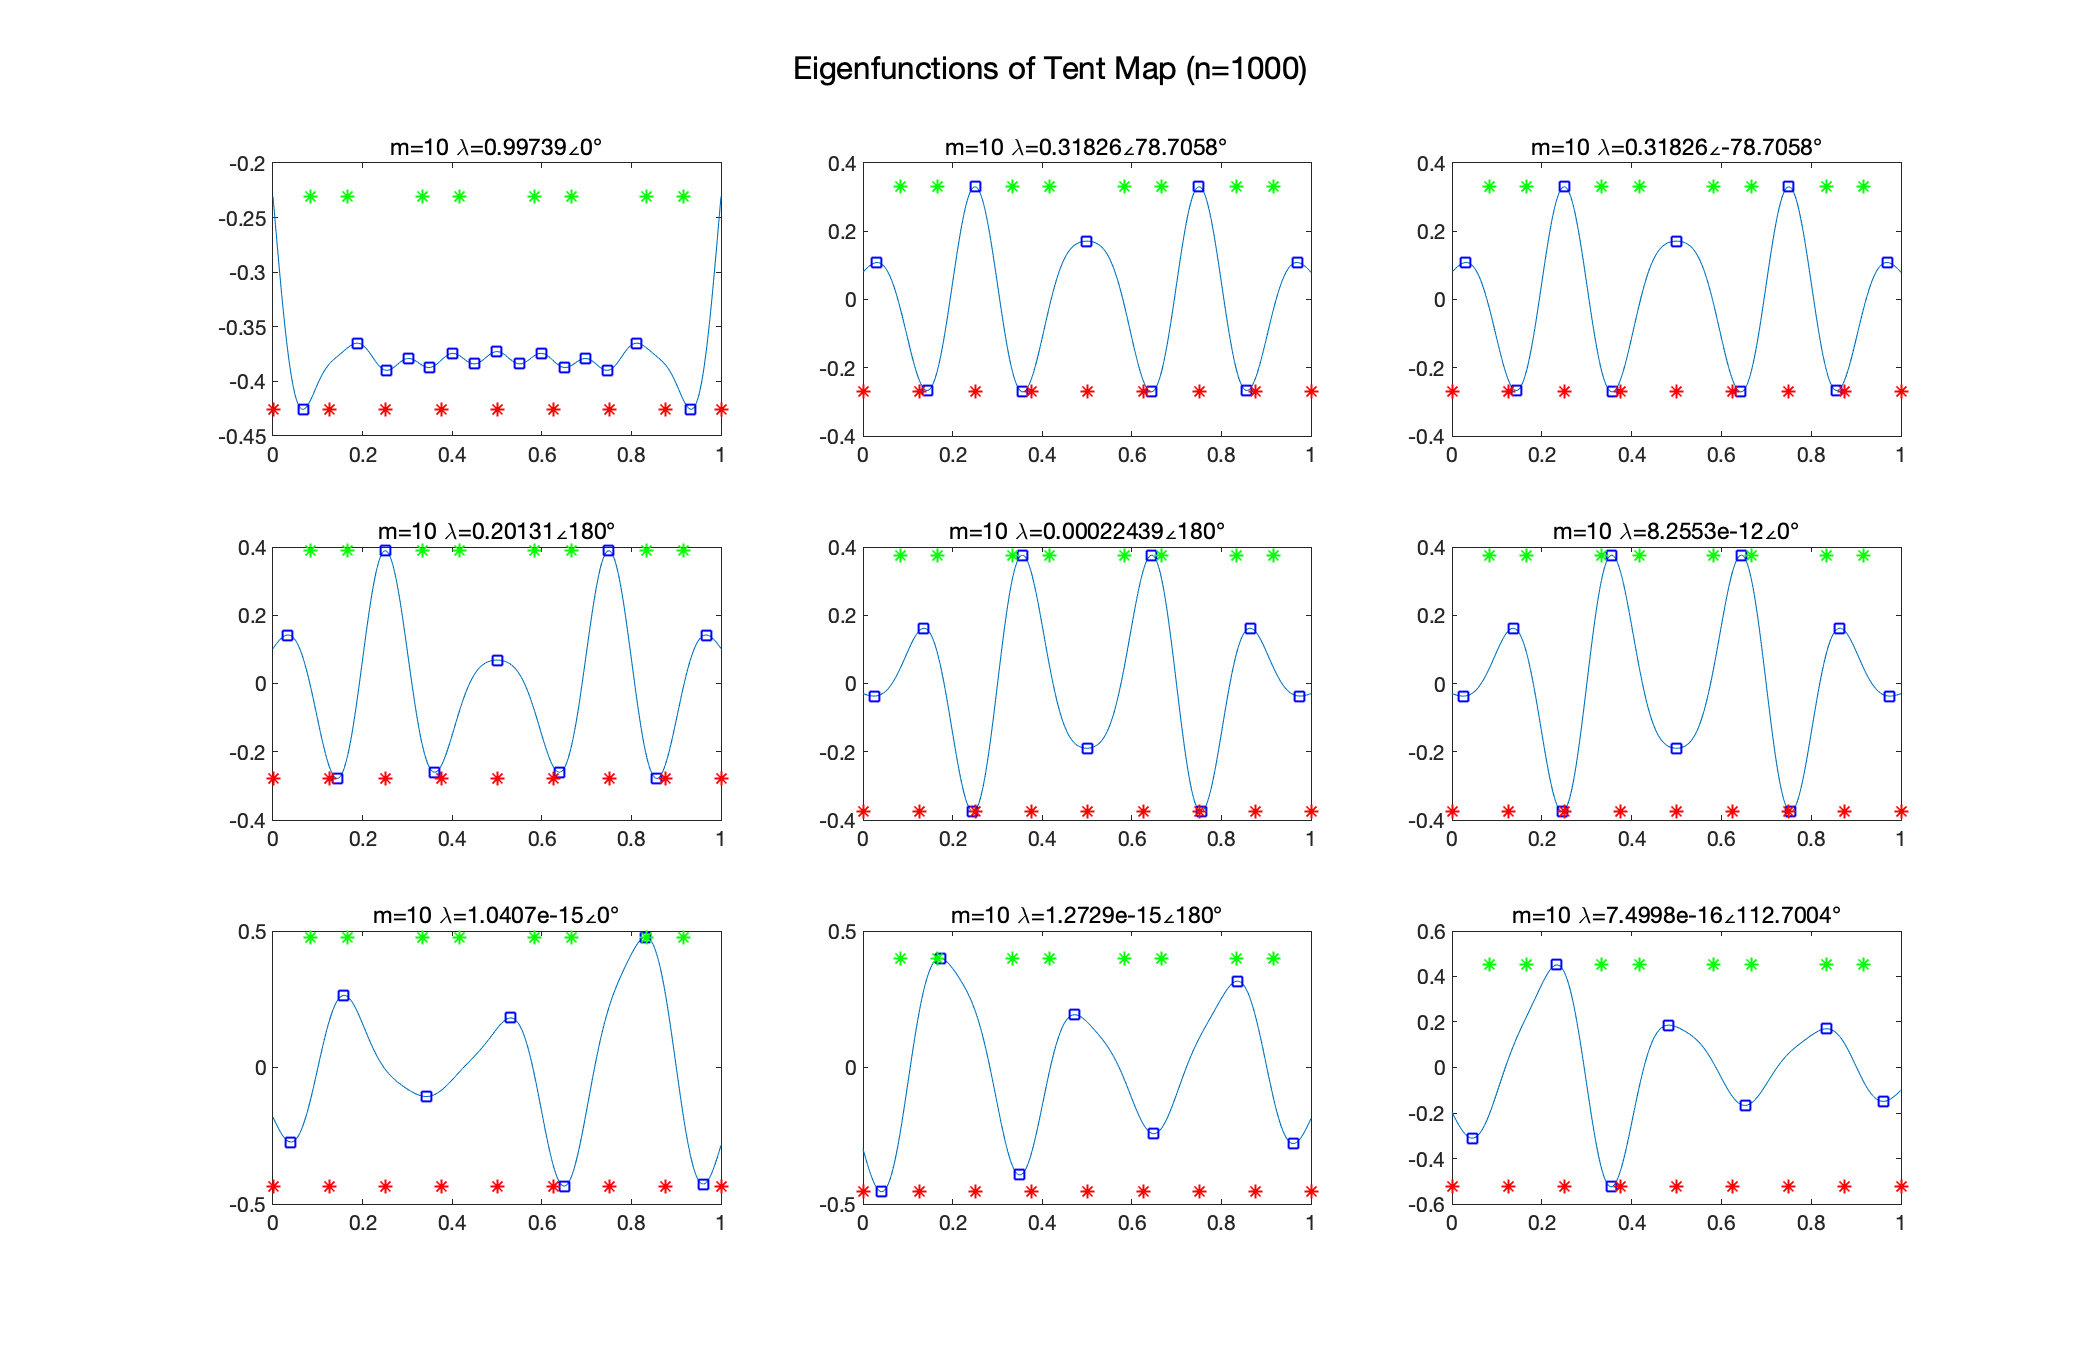
\includegraphics[scale=0.2]{tent/noise/Tent_eigen_noise_n1000m10d0}}
    \\
  \subfloat[m=15]{
    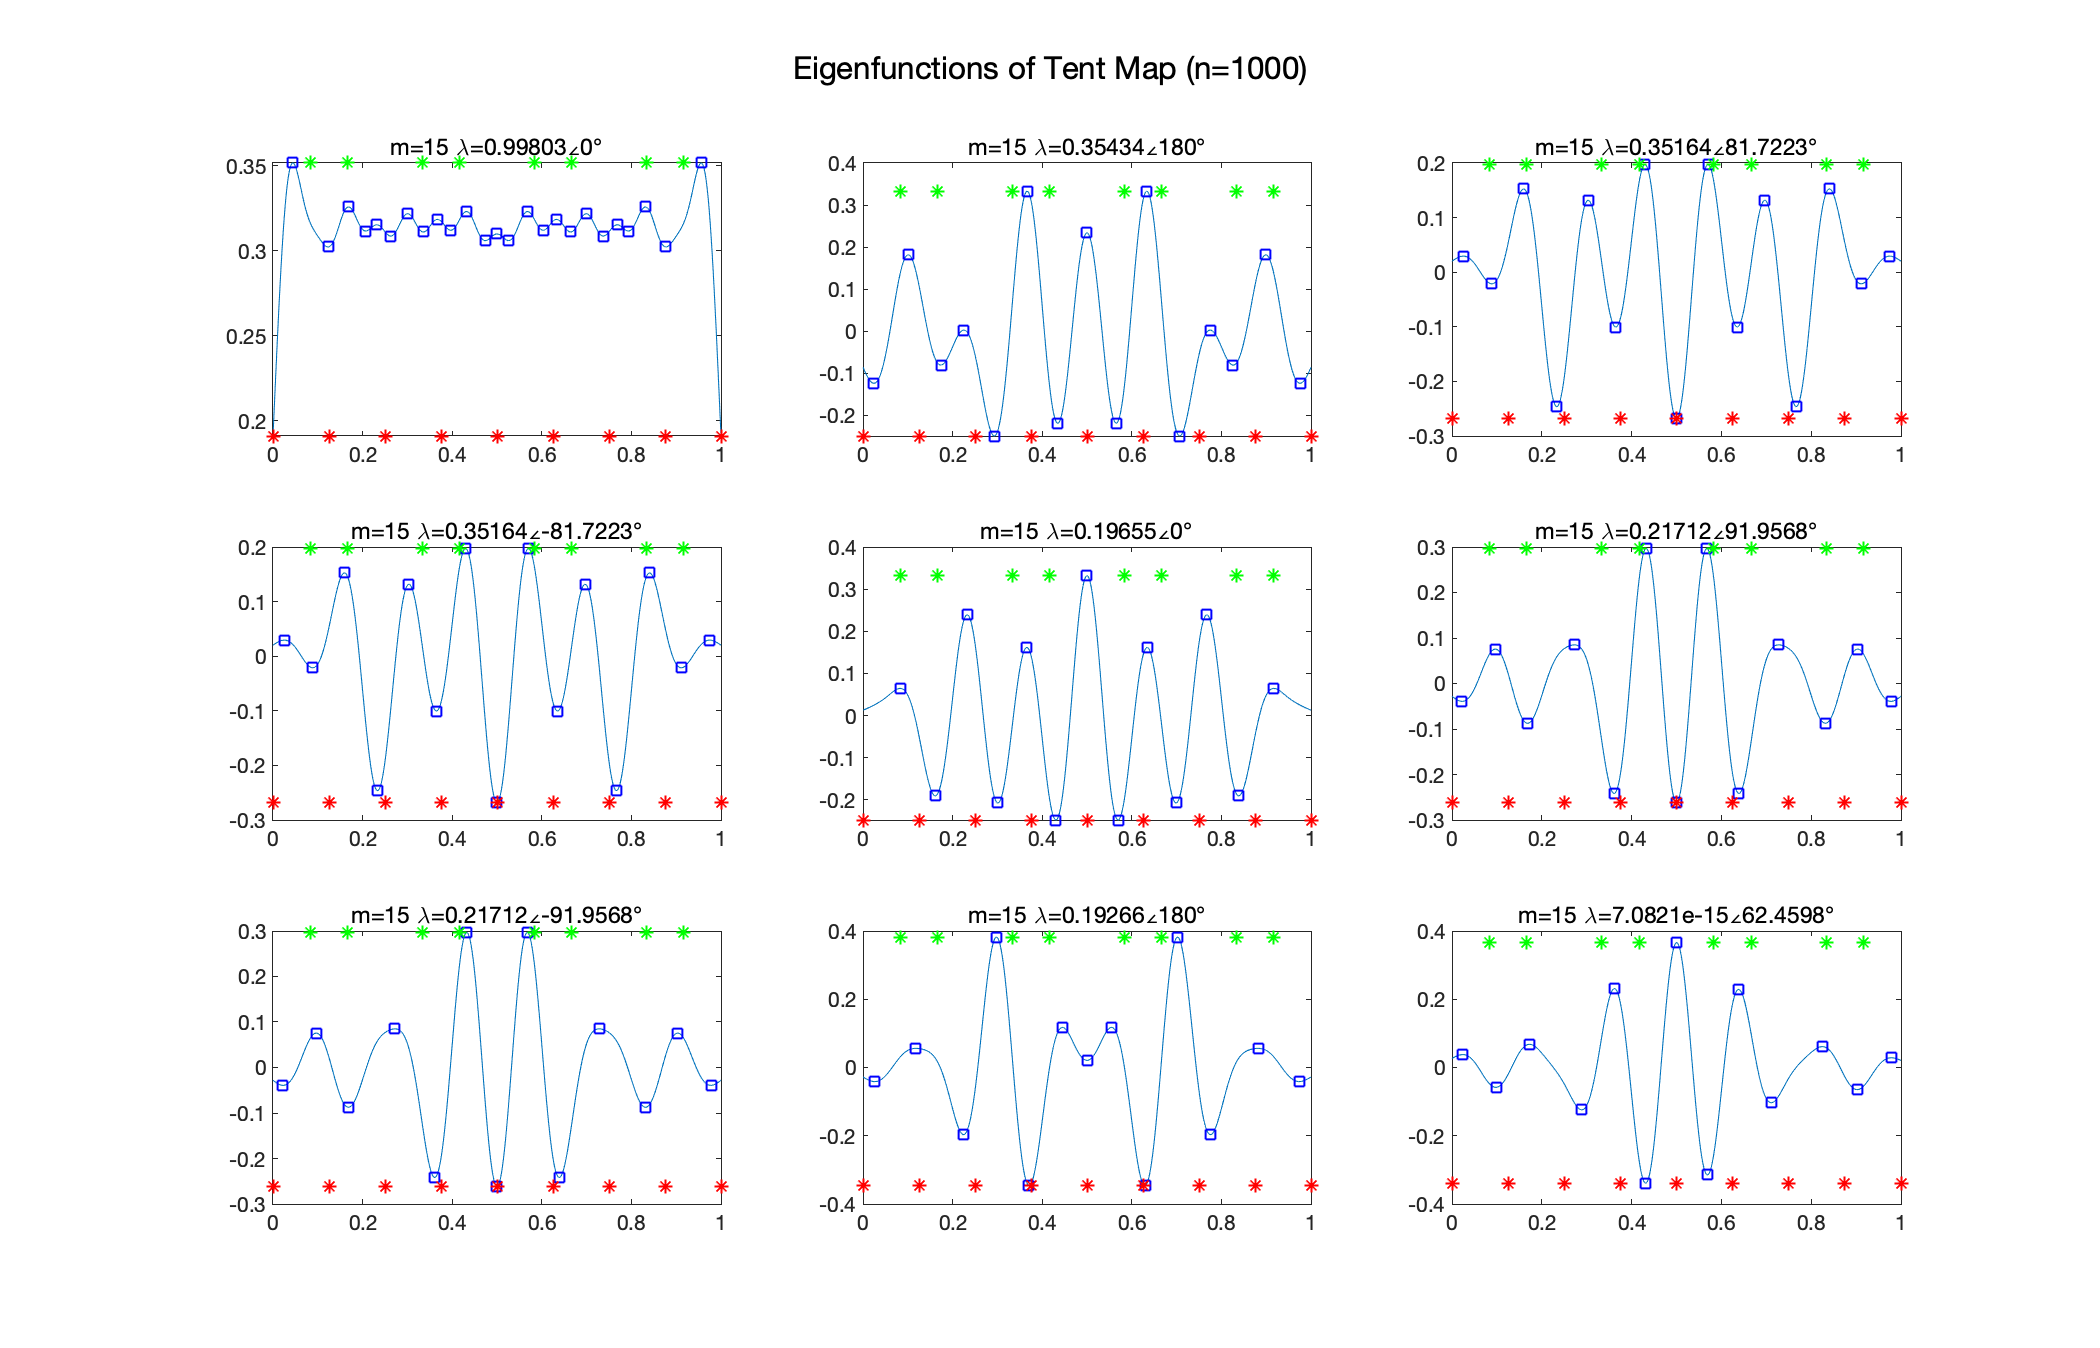
\includegraphics[scale=0.2]{tent/noise/Tent_eigen_noise_n1000m15d0}}
  \subfloat[m=20]{
    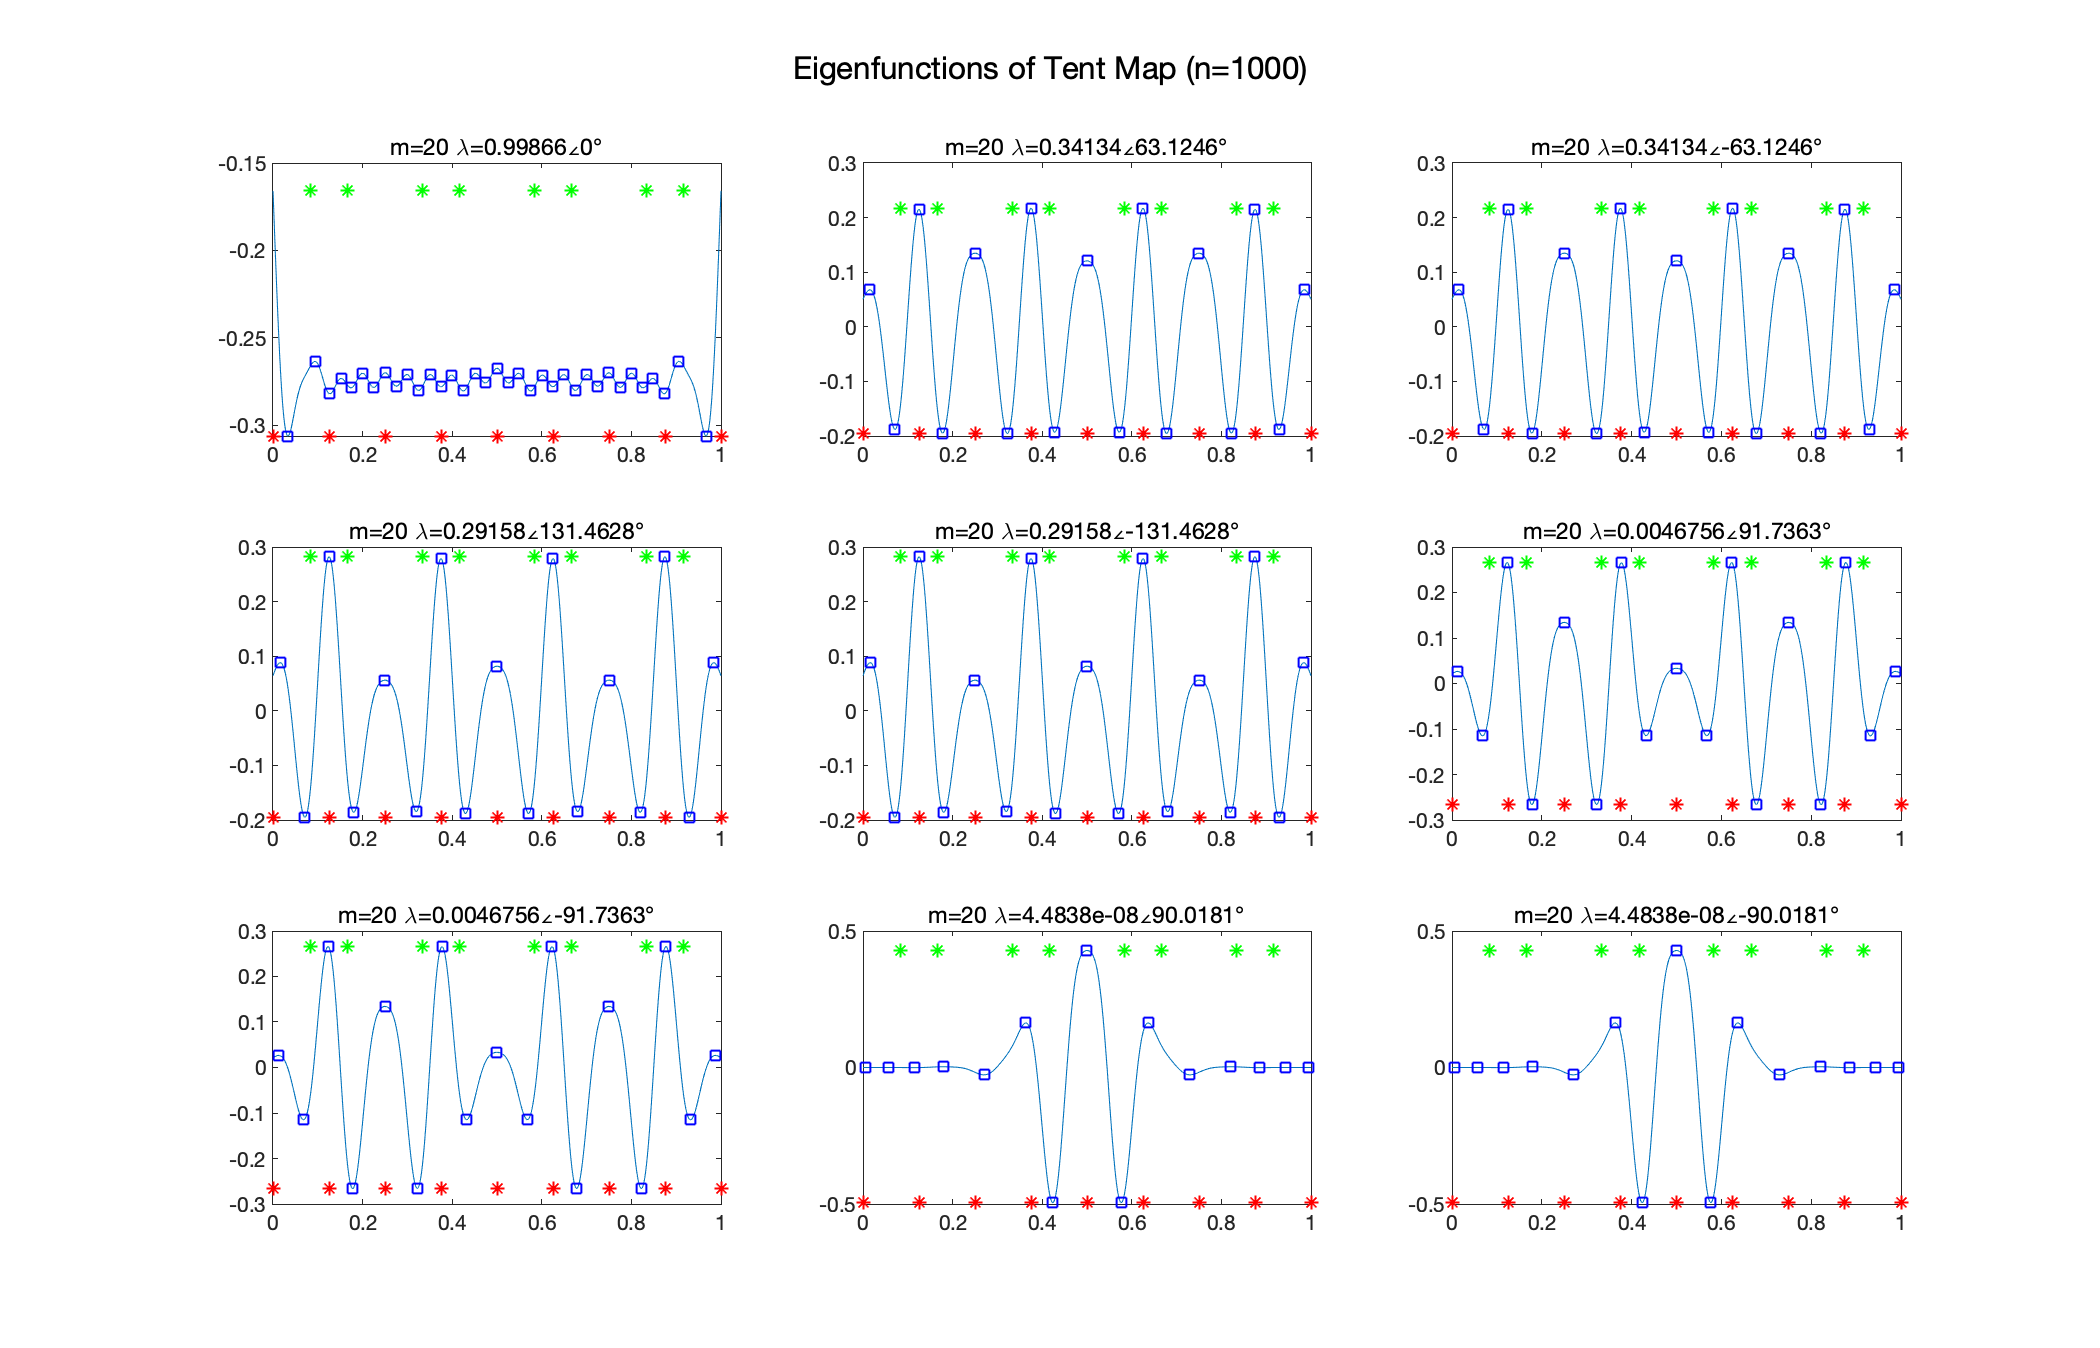
\includegraphics[scale=0.2]{tent/noise/Tent_eigen_noise_n1000m20d0}}
    \\
  \caption{帐篷映射的边界点与本征函数}
\end{figure}

\subsection{更多的讨论}
\subsubsection{噪声对Koopman算符的影响}

\begin{figure}
  \centering
  \subfloat[noise=0]{
    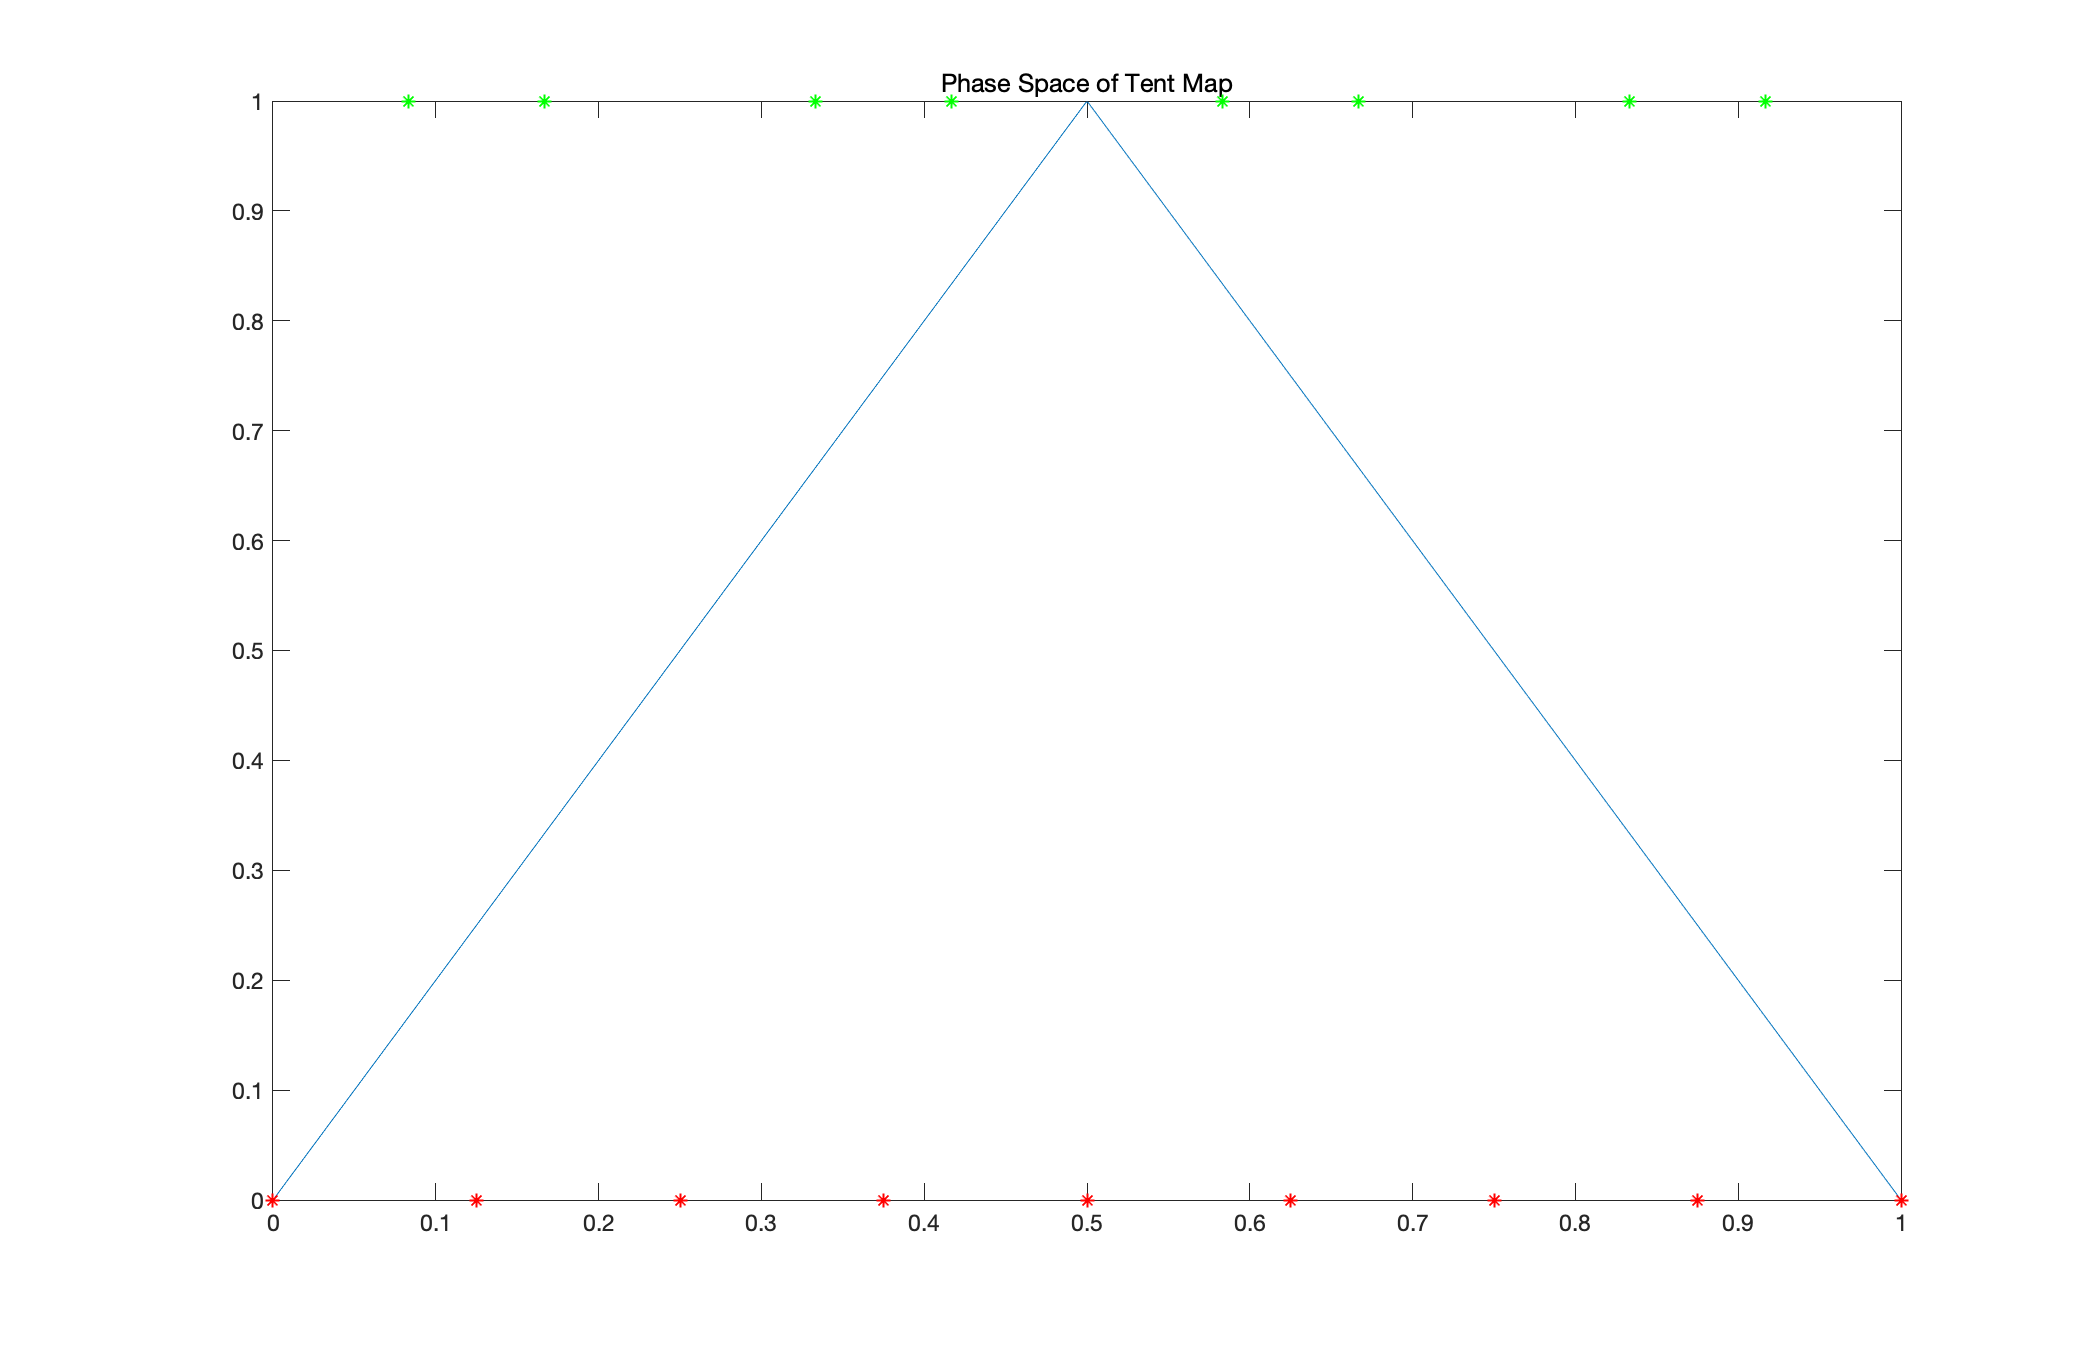
\includegraphics[scale=0.13]{tent/noise/Tent_noise_phase_d0}}
  \subfloat[noise=0.001]{
    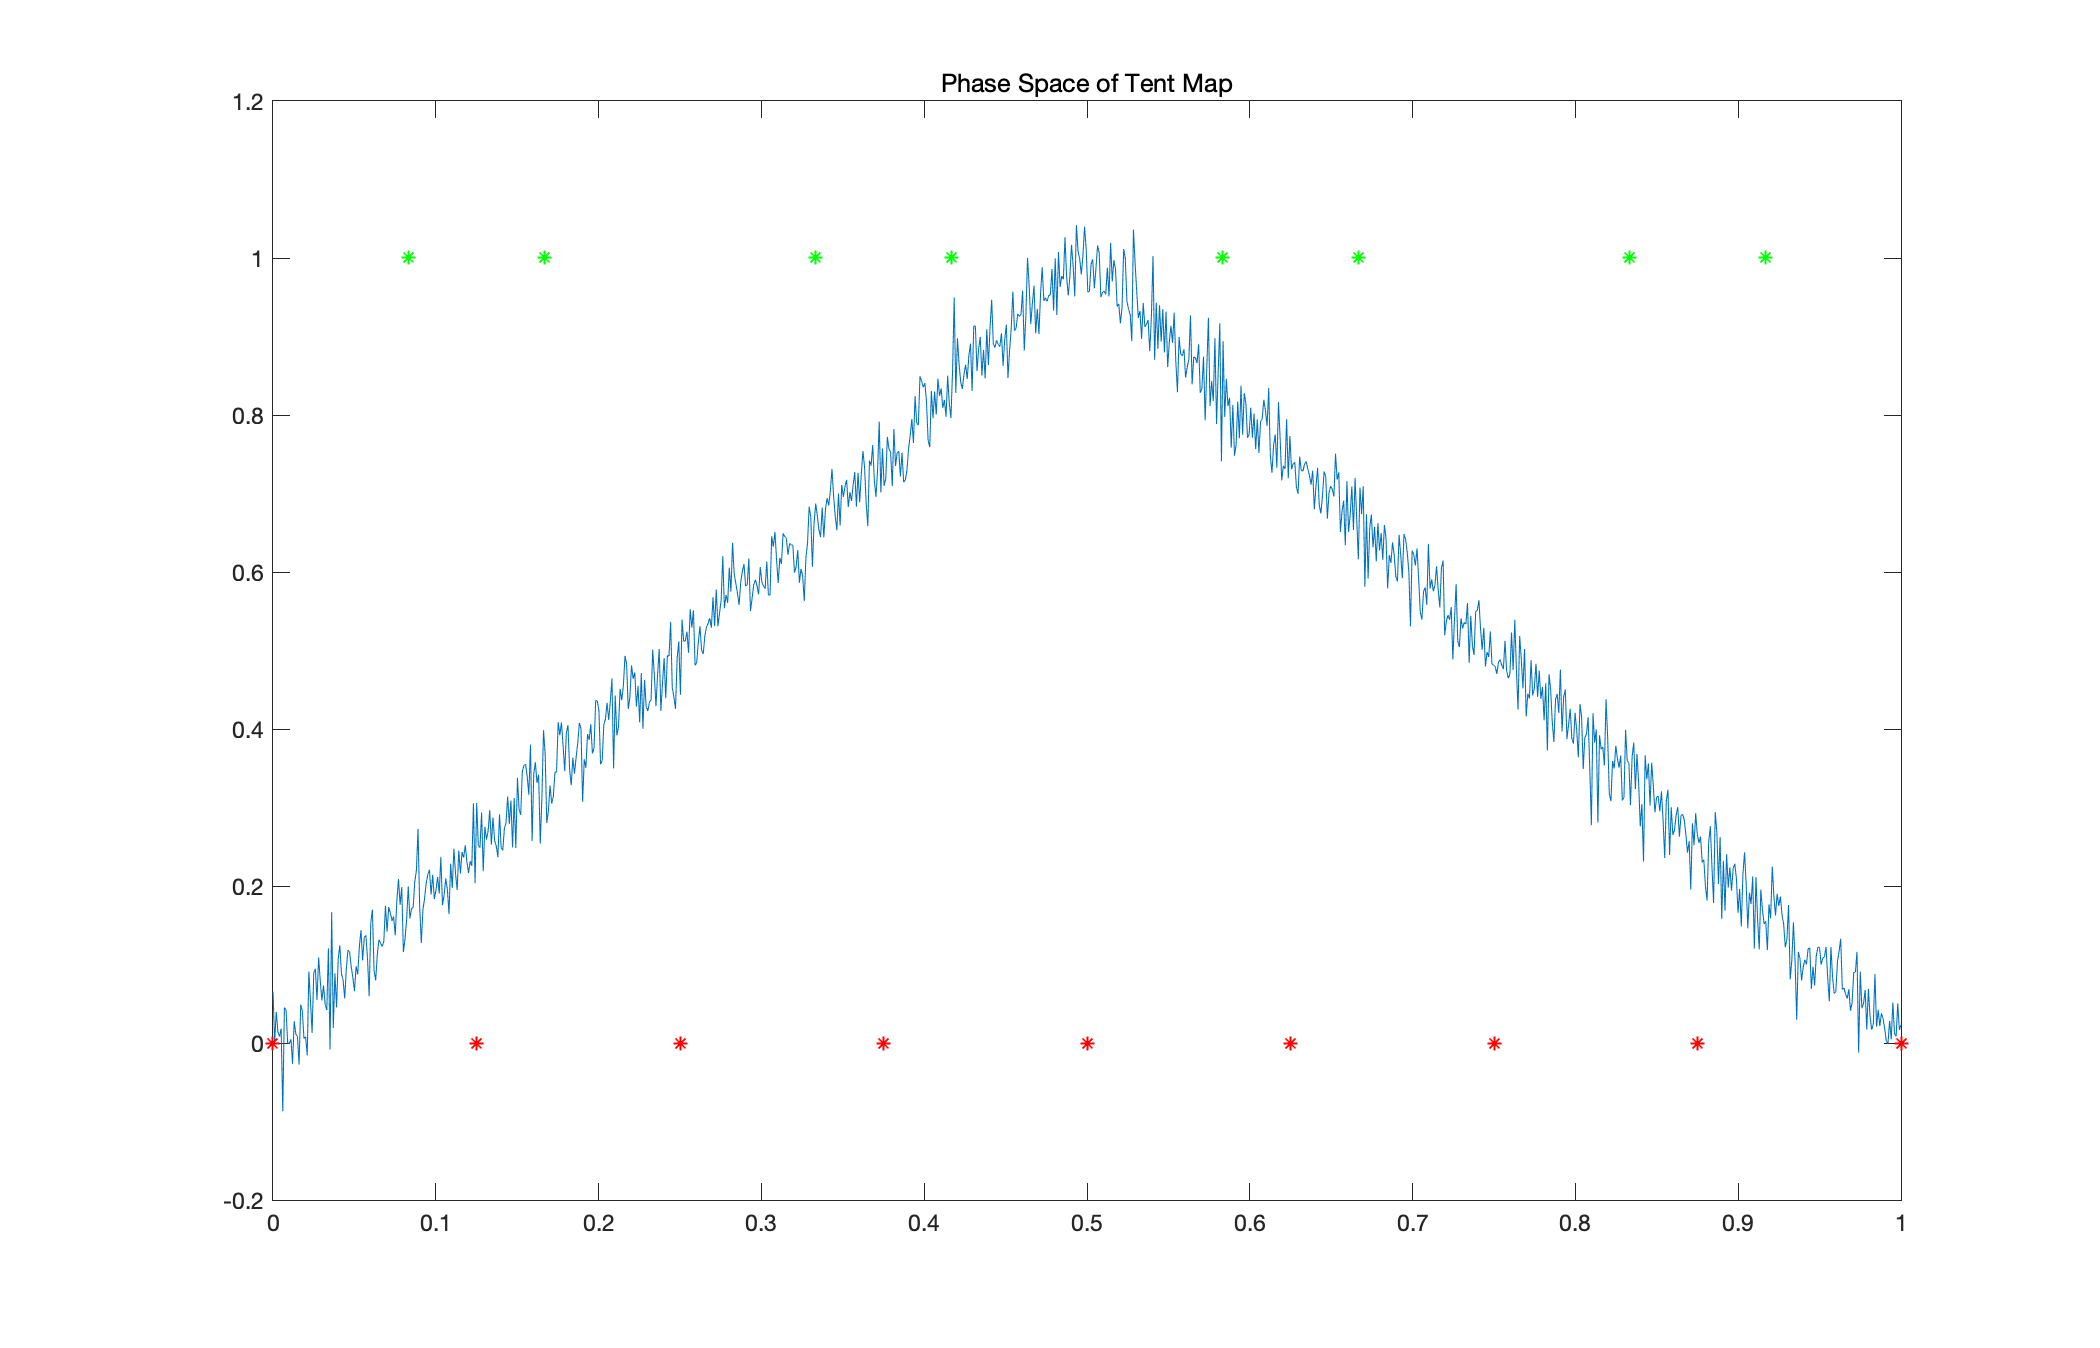
\includegraphics[scale=0.13]{tent/noise/Tent_noise_phase_d0-001}}
  \subfloat[noise=0.01]{
    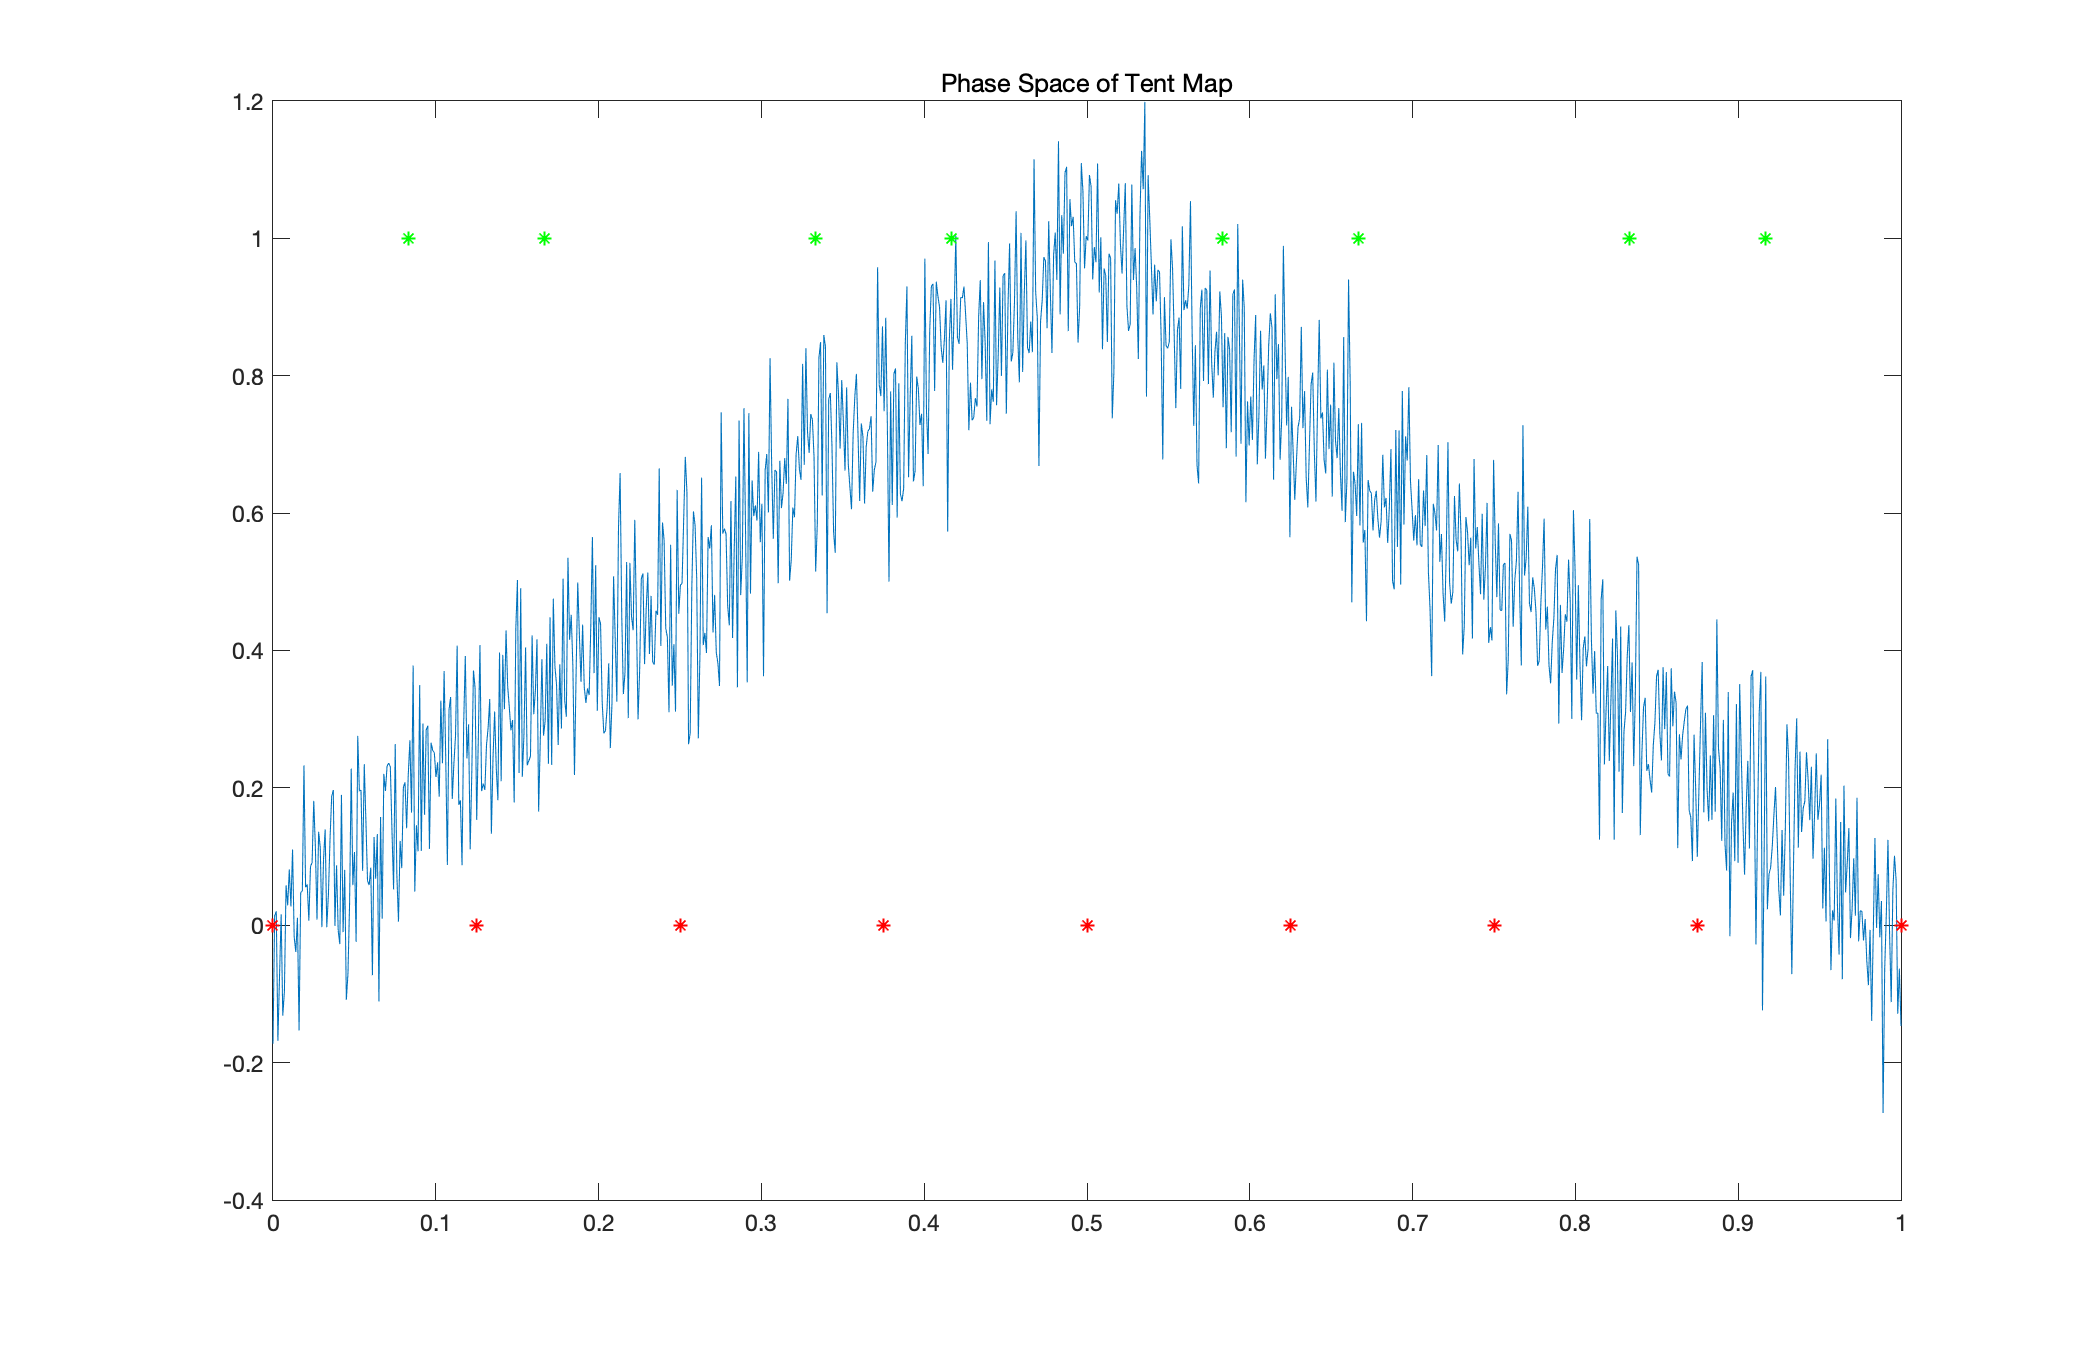
\includegraphics[scale=0.13]{tent/noise/Tent_noise_phase_d0-01}}
  \caption{帐篷映射不同噪声下的相空间}
\end{figure}

\begin{figure}
  \centering%[2,3,4,5,8,10,15,20]
  \subfloat[m=2]{
    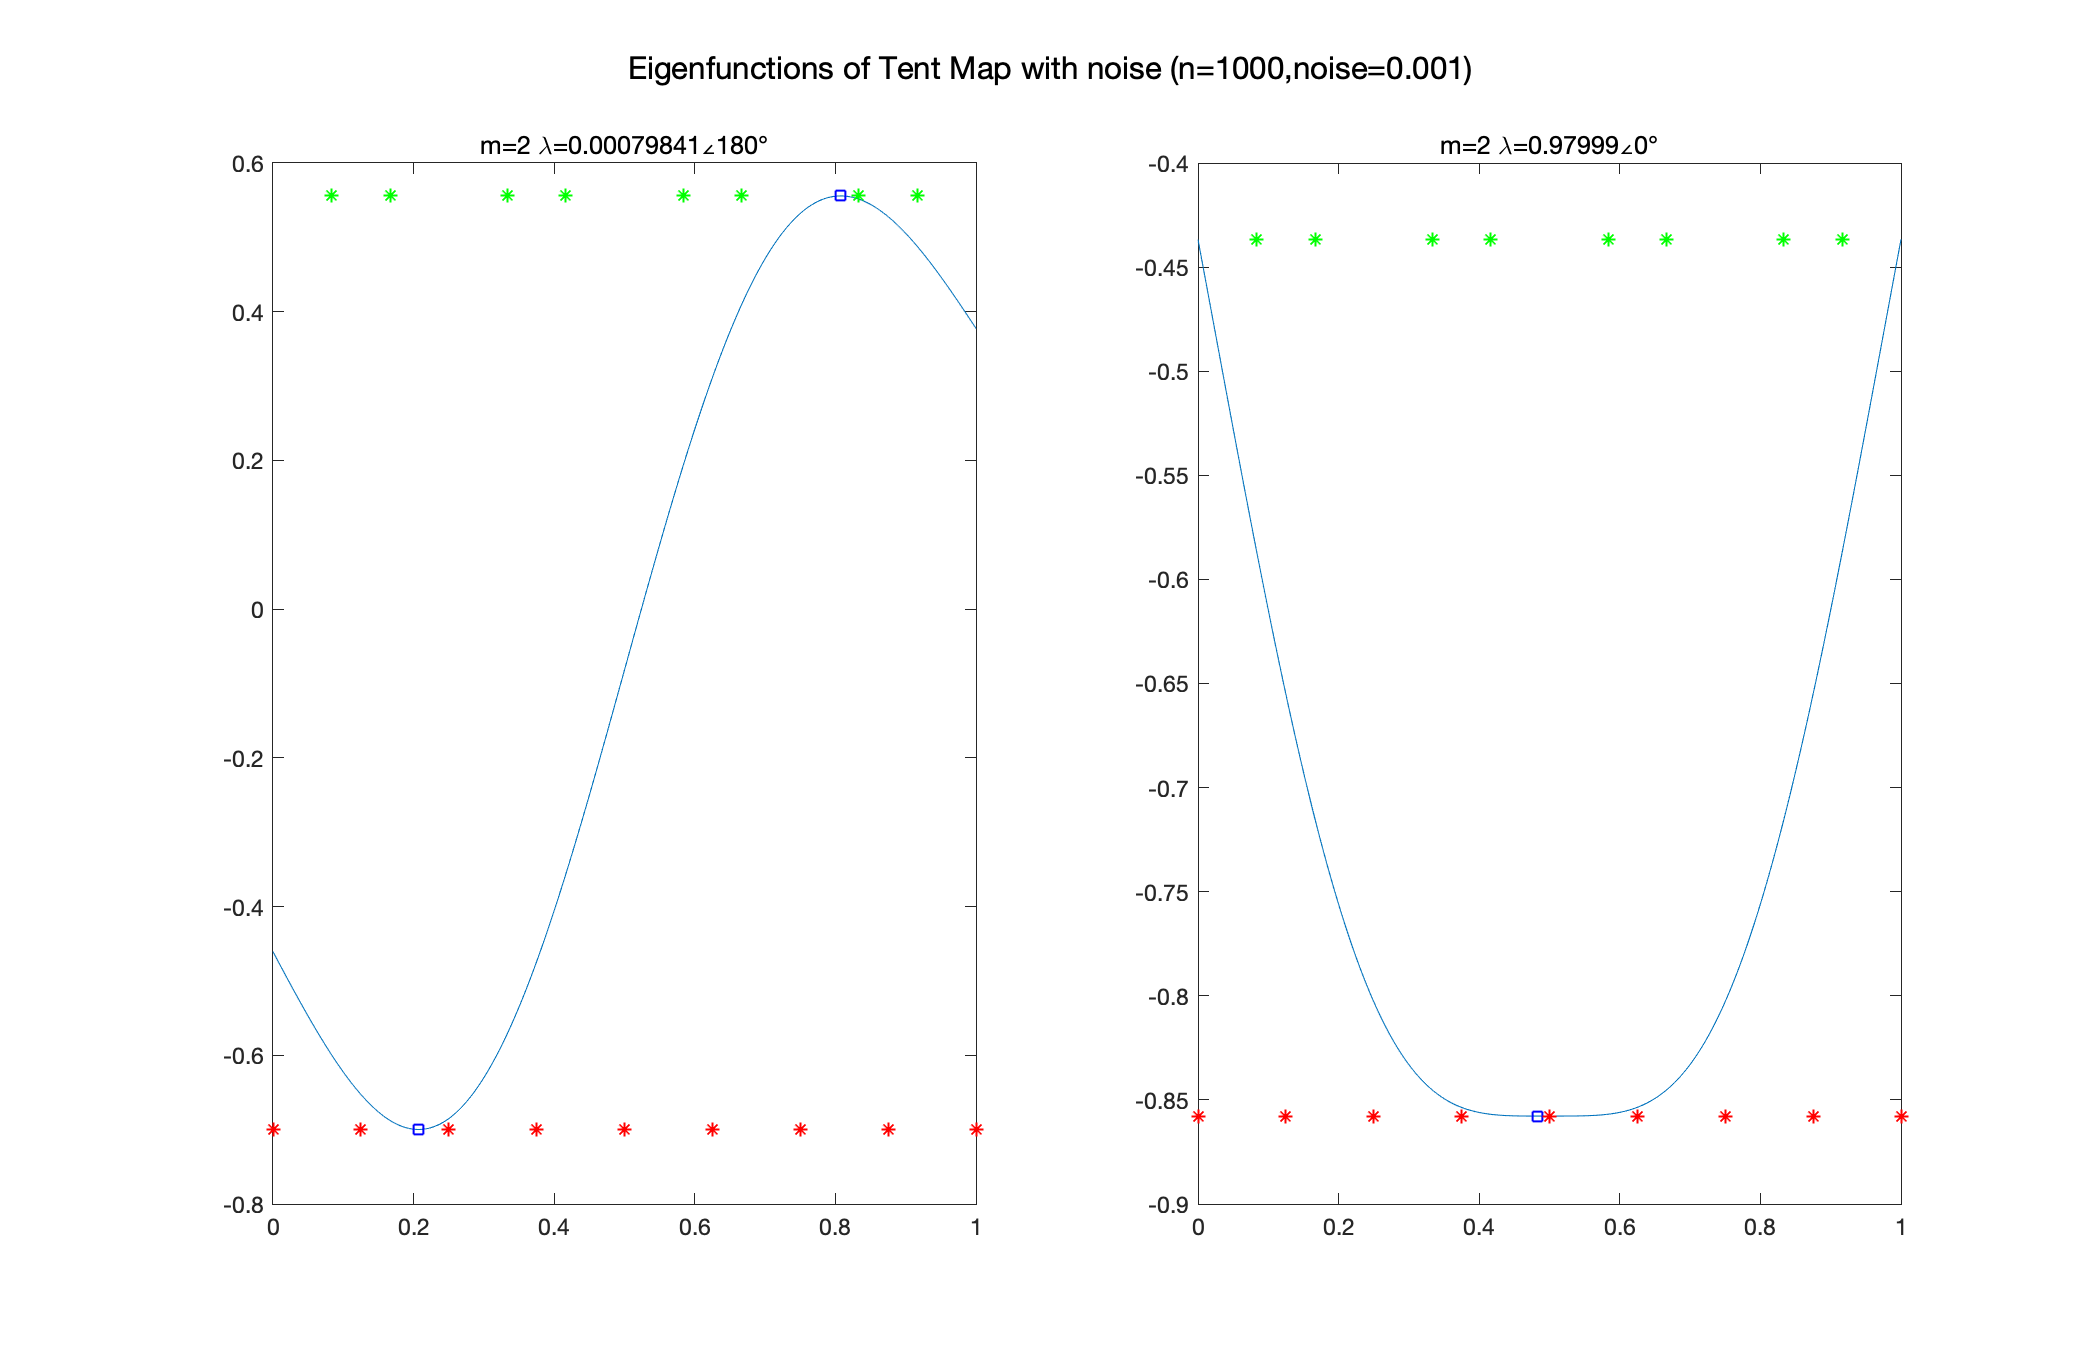
\includegraphics[scale=0.2]{tent/noise/Tent_eigen_noise_n1000m2d0-001}}
  \subfloat[m=3]{
    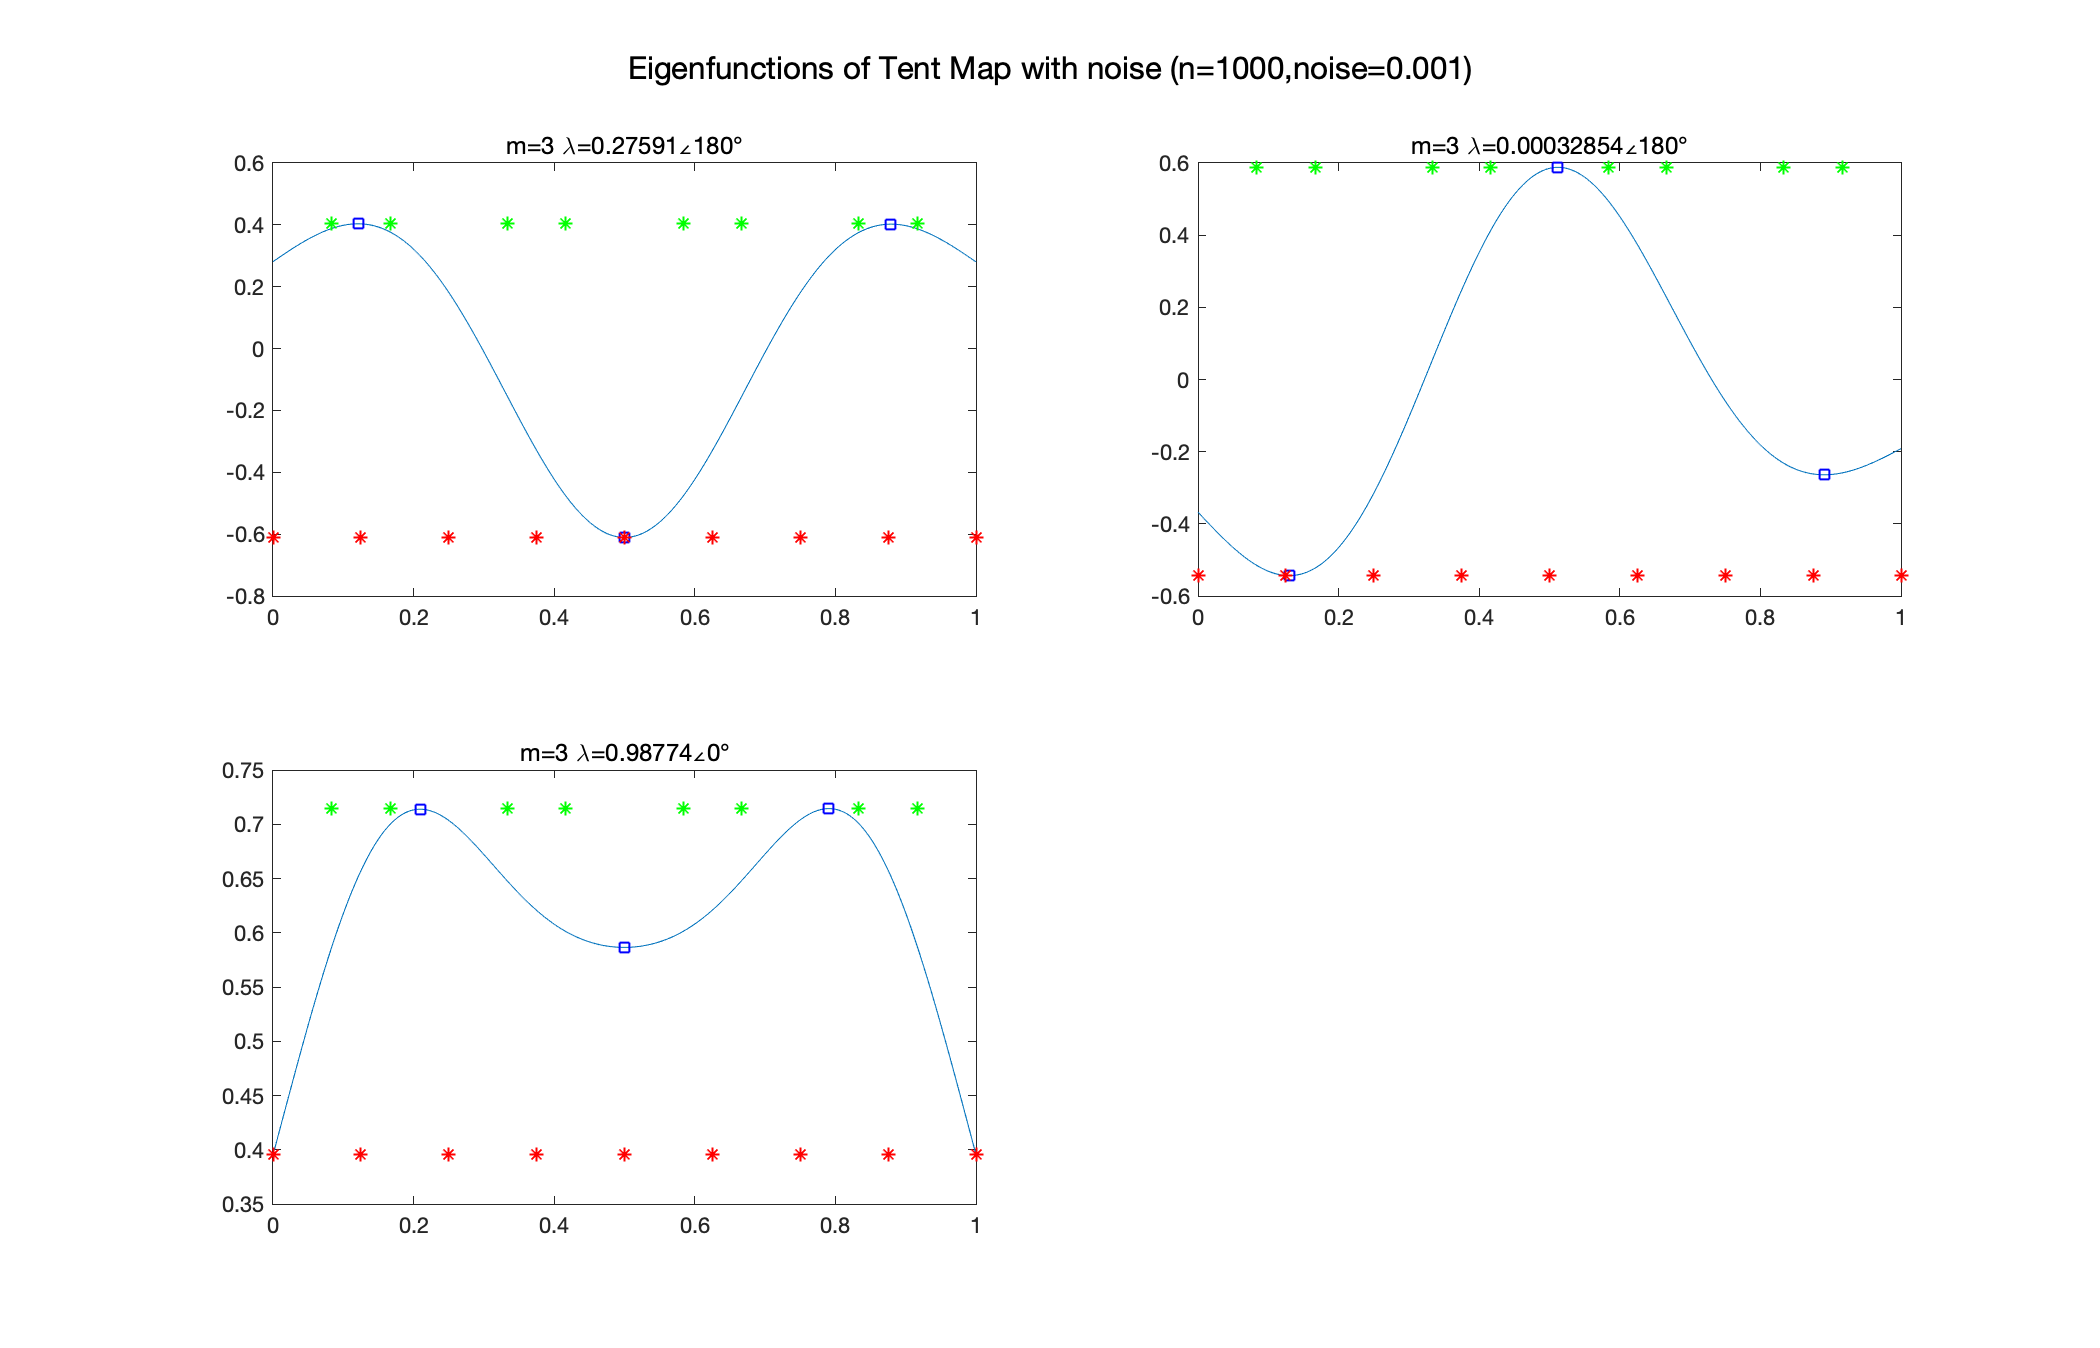
\includegraphics[scale=0.2]{tent/noise/Tent_eigen_noise_n1000m3d0-001}}
    \\
  \subfloat[m=4]{
    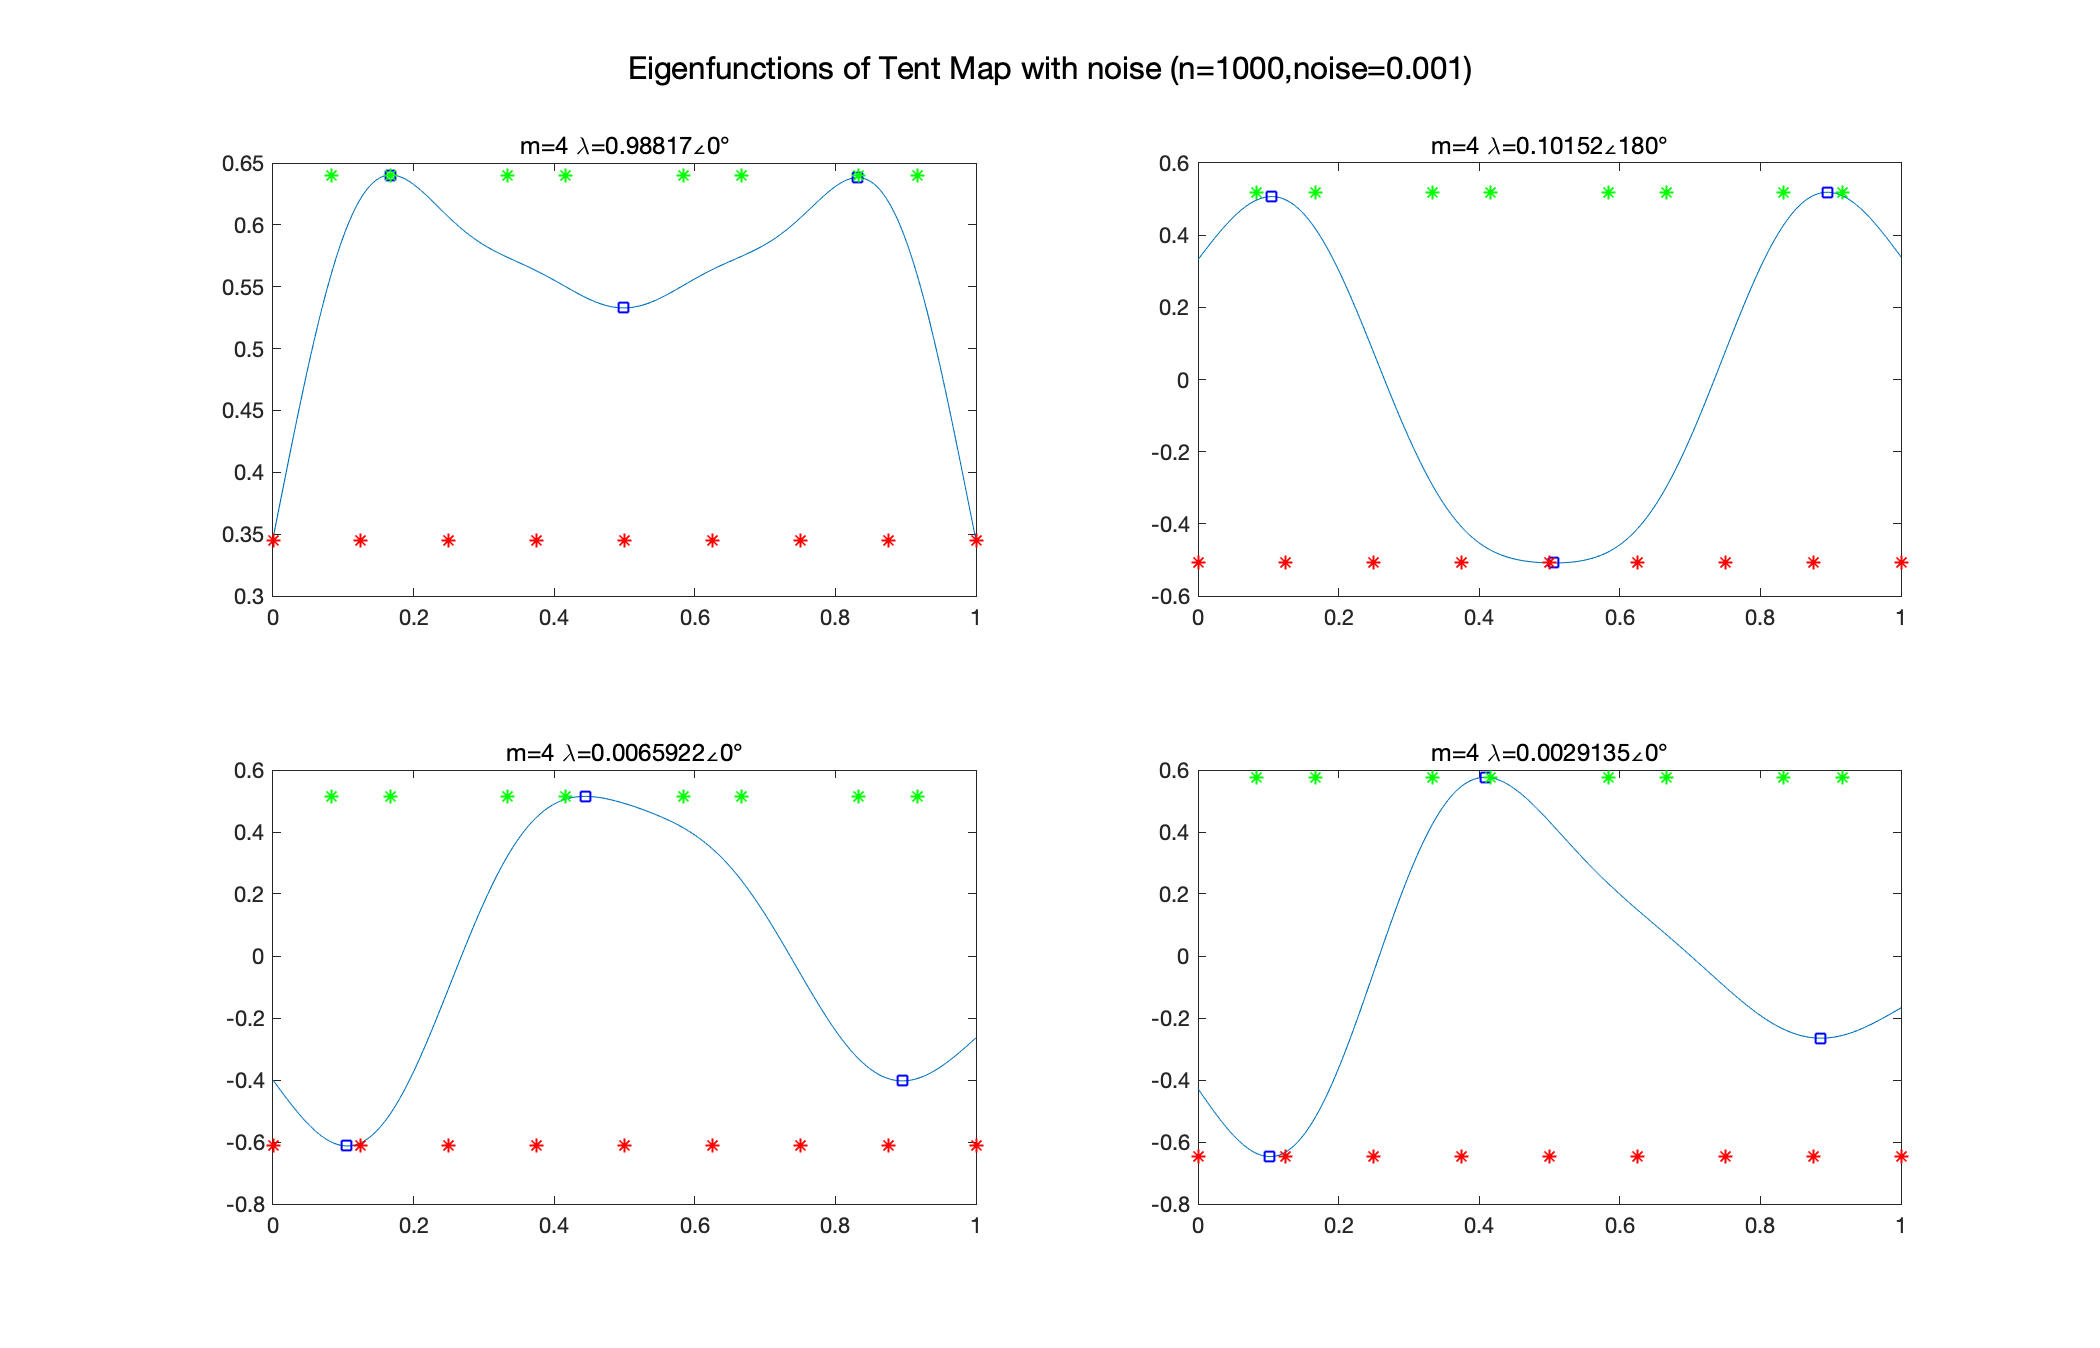
\includegraphics[scale=0.2]{tent/noise/Tent_eigen_noise_n1000m4d0-001}}
  \subfloat[m=5]{
    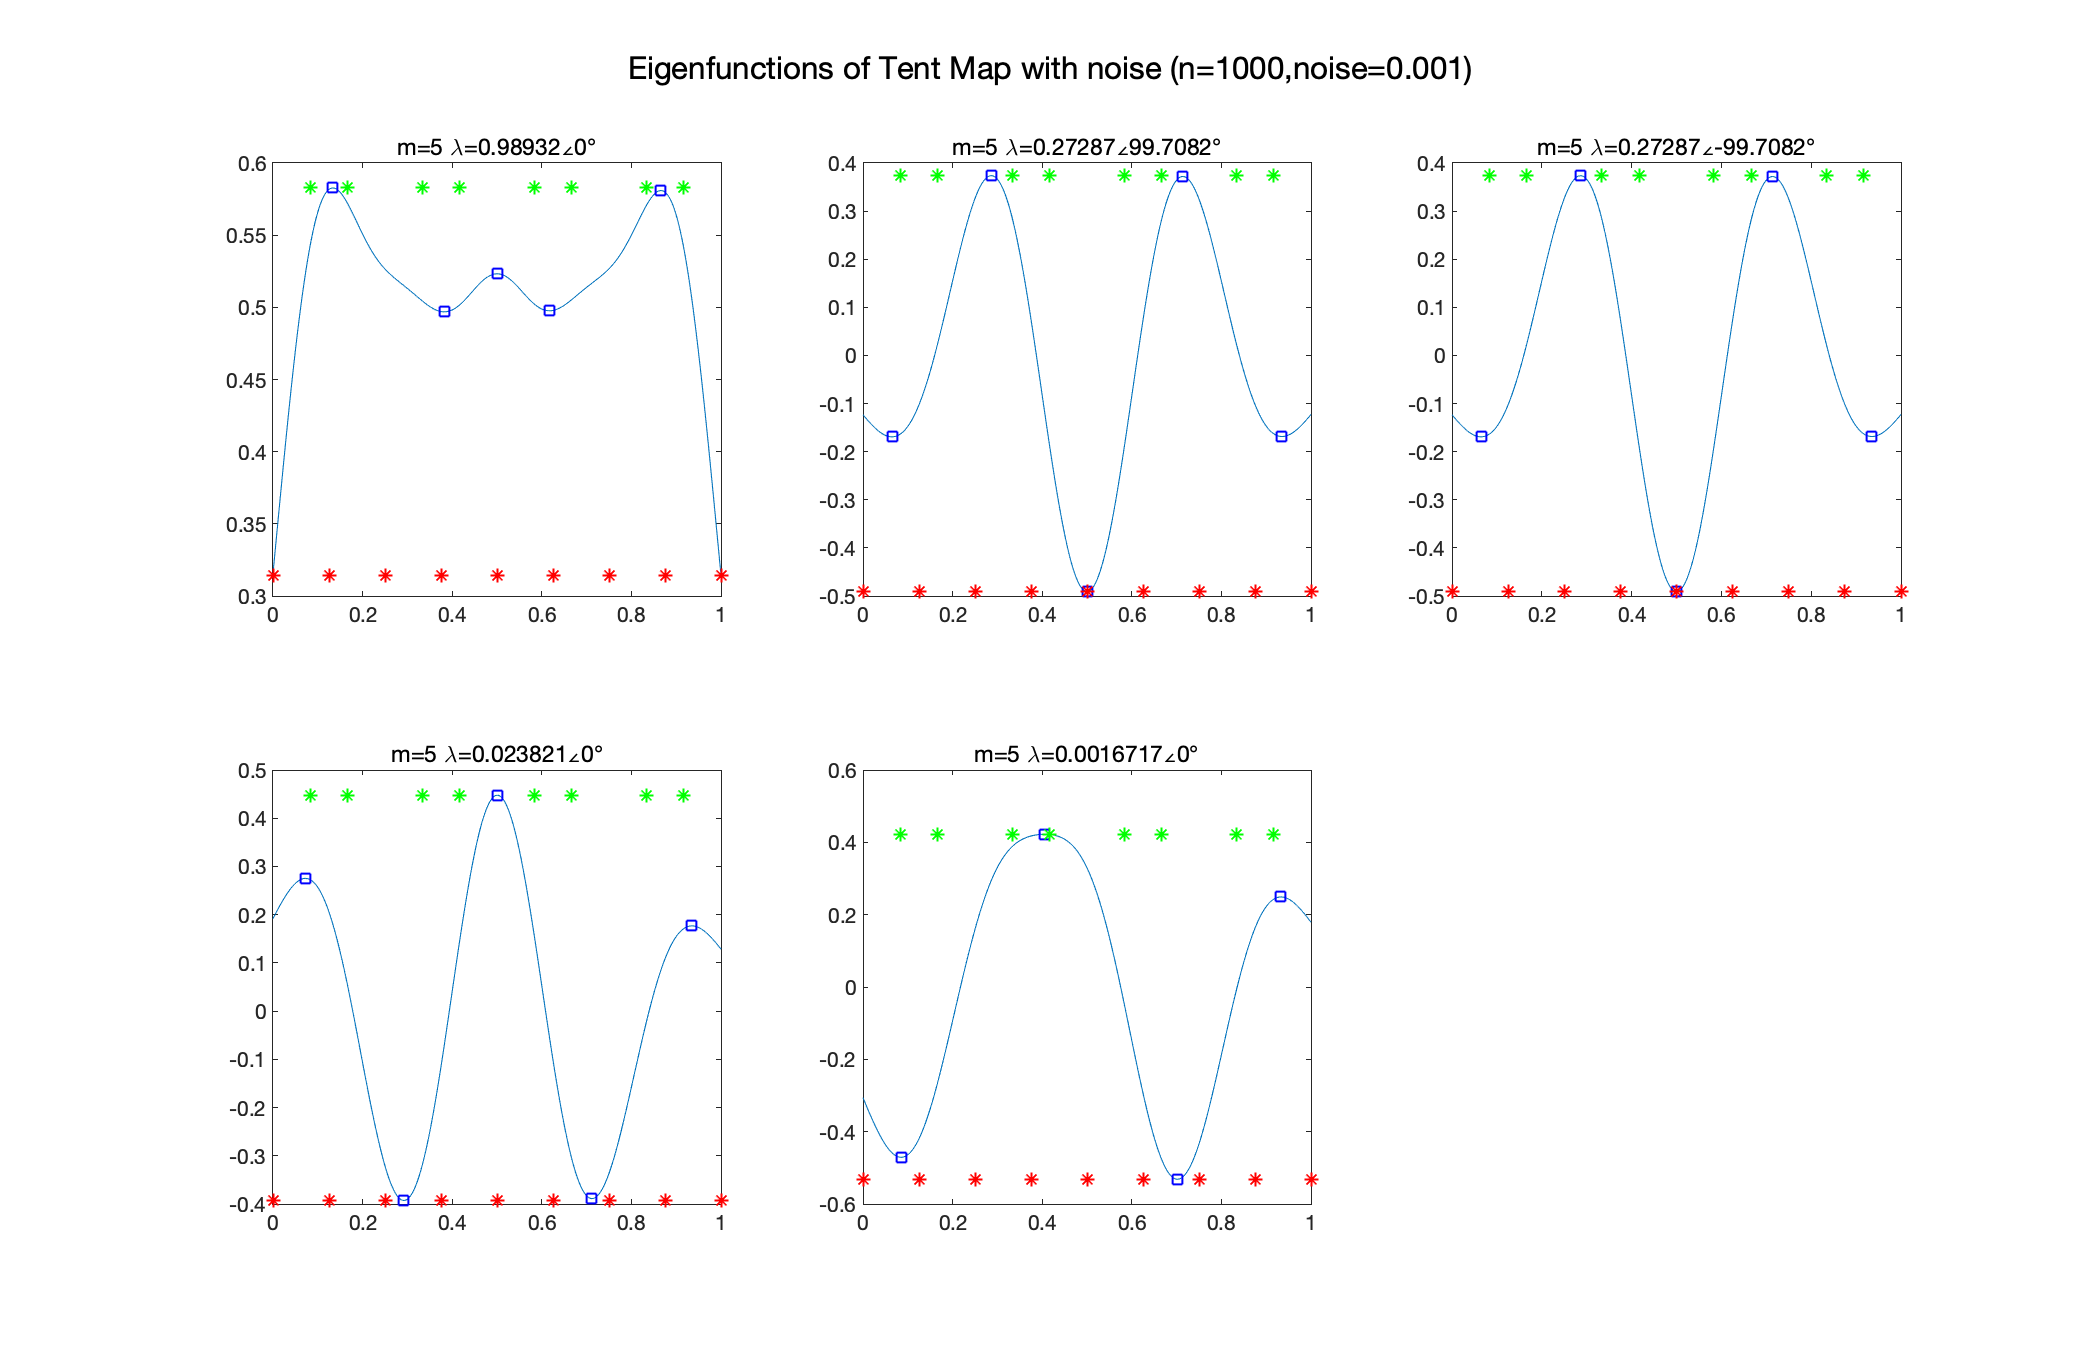
\includegraphics[scale=0.2]{tent/noise/Tent_eigen_noise_n1000m5d0-001}}
    \\
  \subfloat[m=8]{
    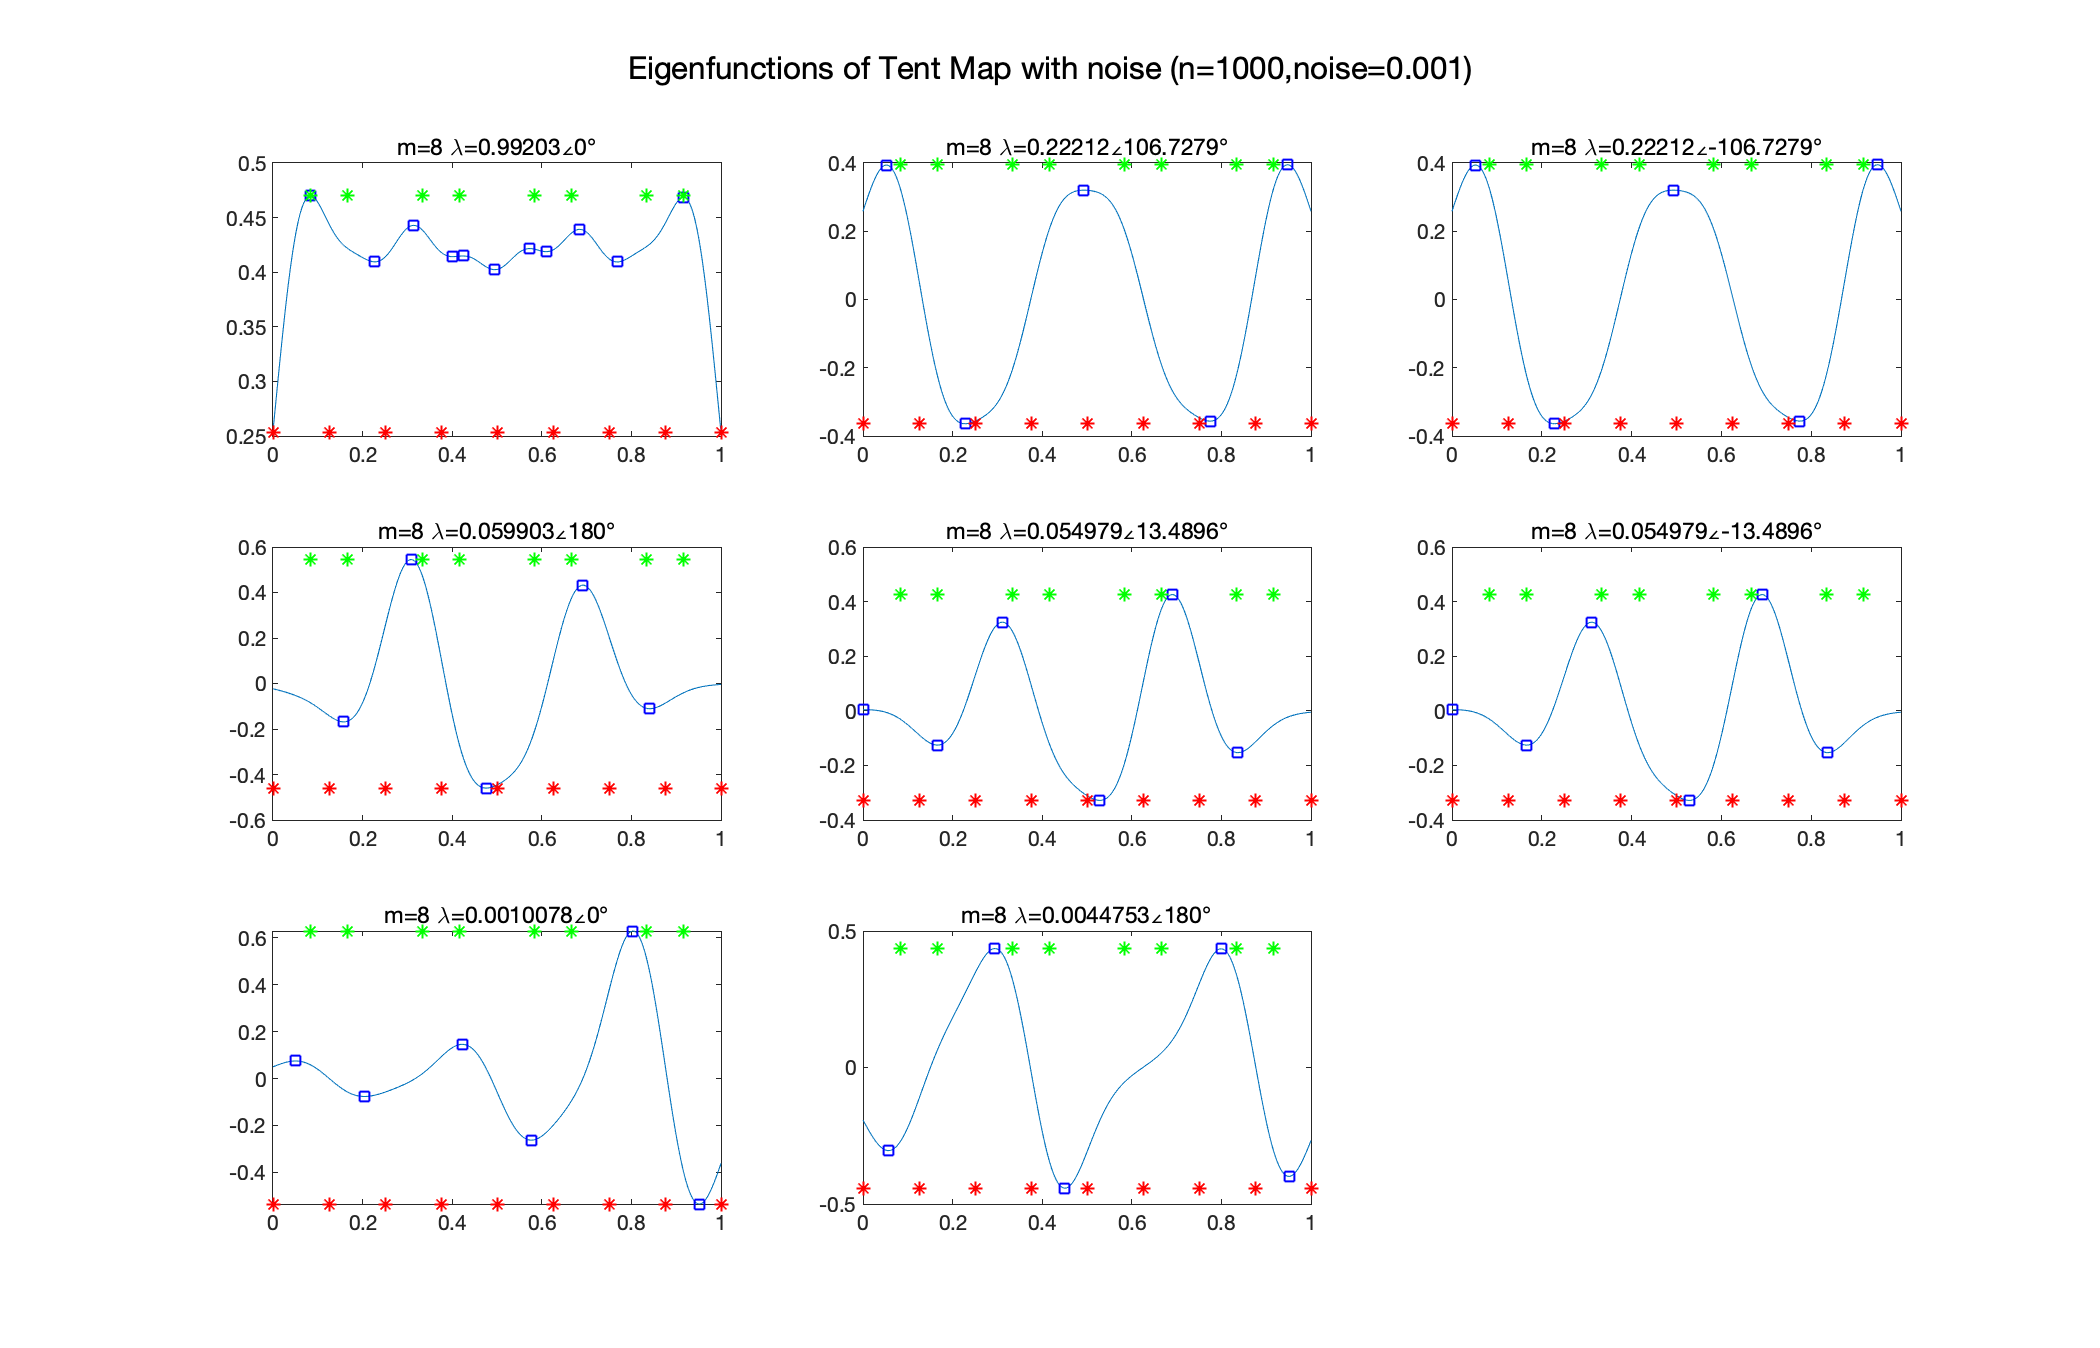
\includegraphics[scale=0.2]{tent/noise/Tent_eigen_noise_n1000m8d0-001}}
  \subfloat[m=10]{
    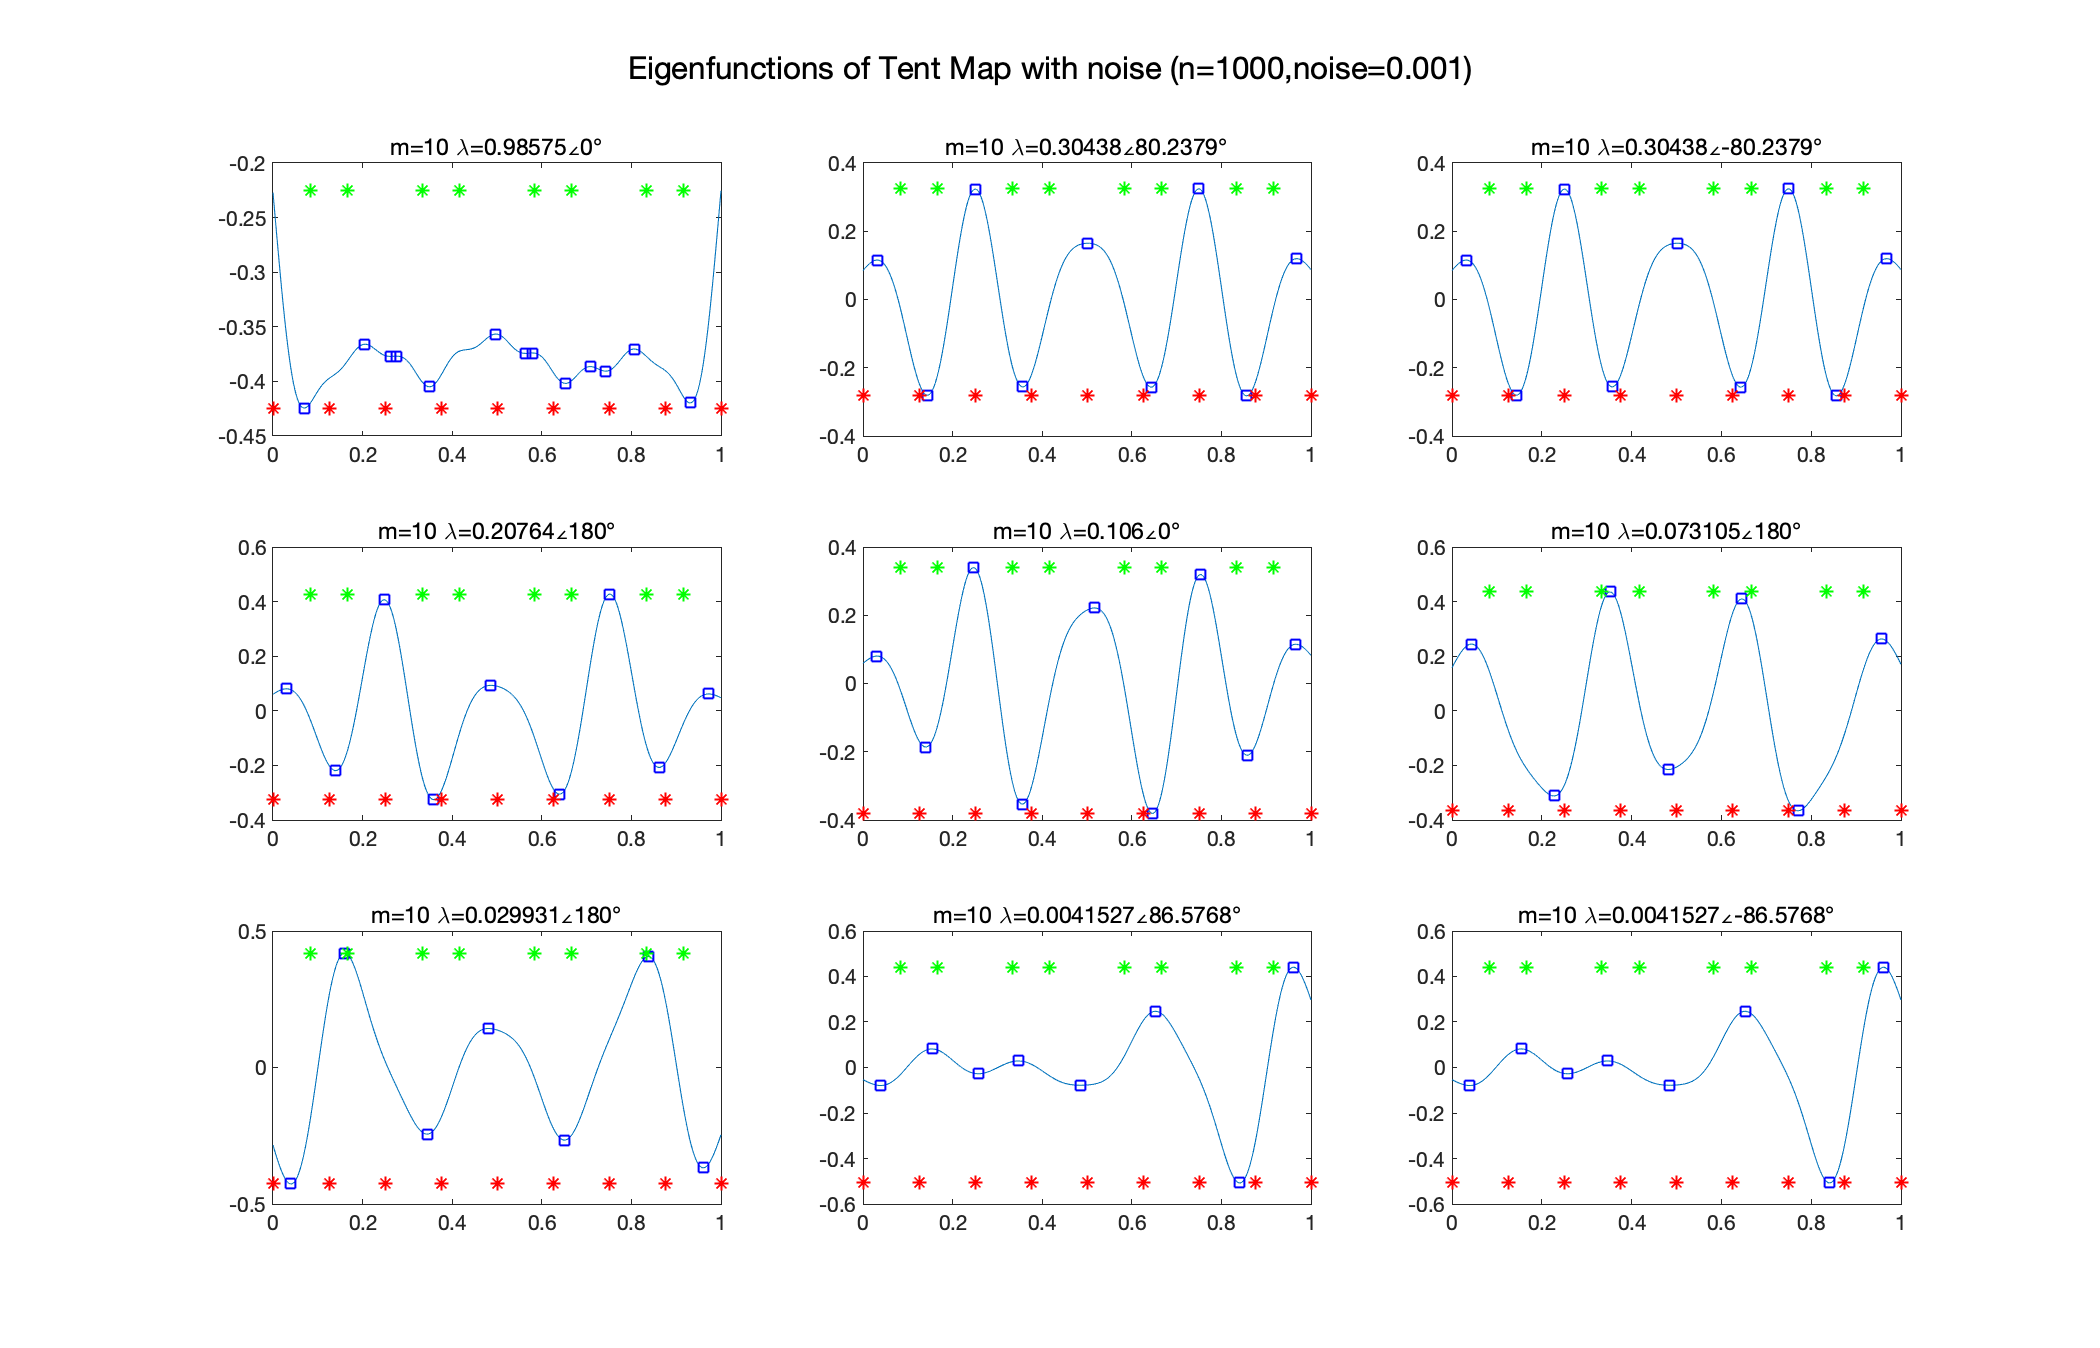
\includegraphics[scale=0.2]{tent/noise/Tent_eigen_noise_n1000m10d0-001}}
    \\
  \subfloat[m=15]{
    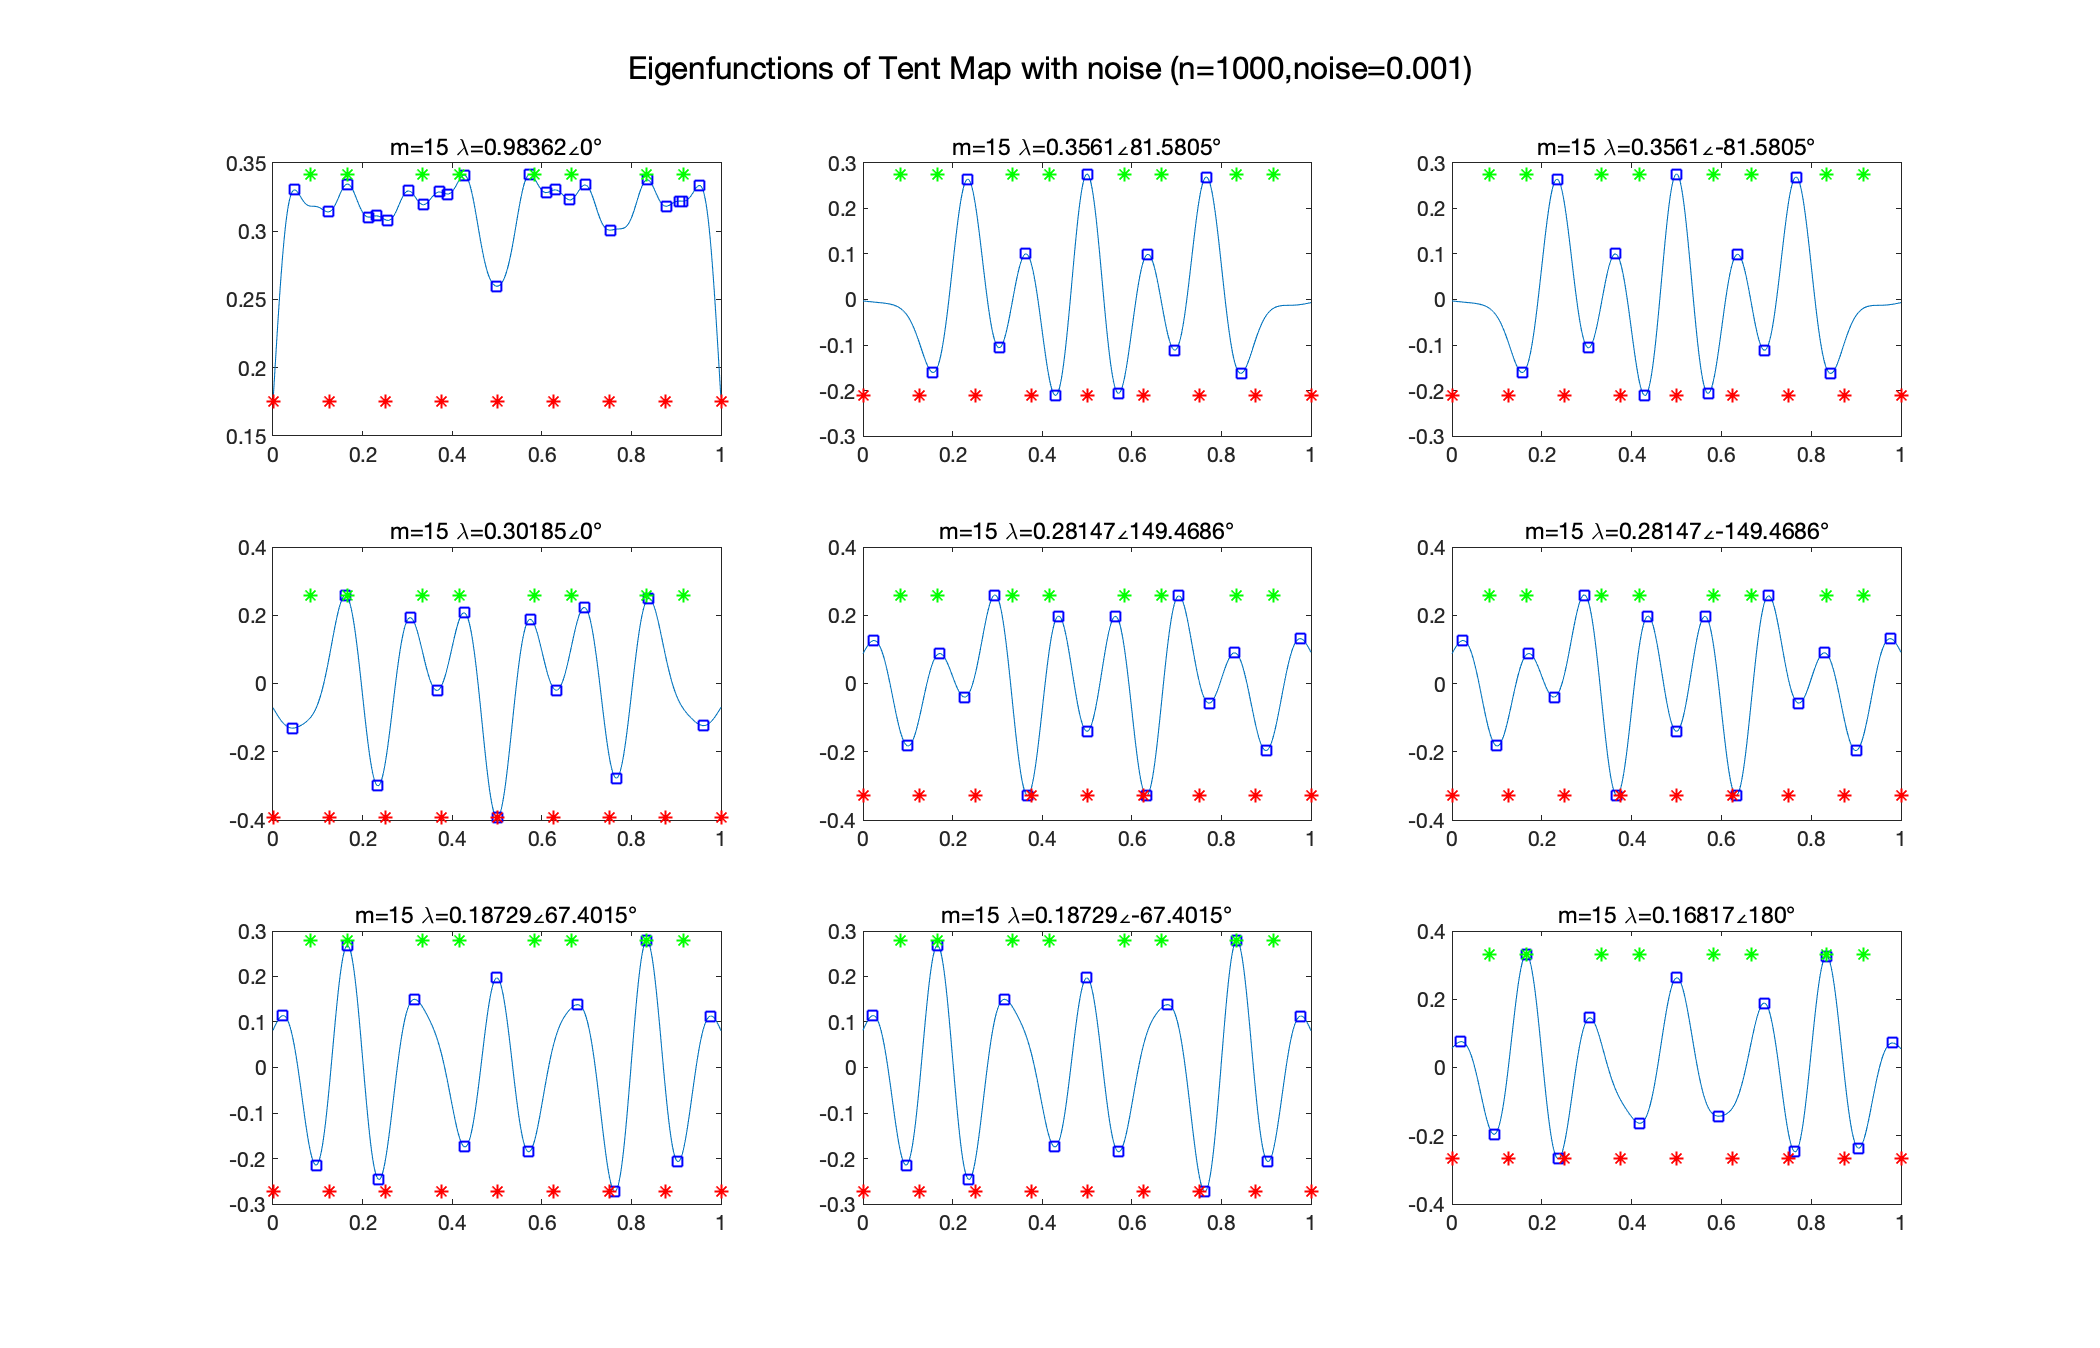
\includegraphics[scale=0.2]{tent/noise/Tent_eigen_noise_n1000m15d0-001}}
  \subfloat[m=20]{
    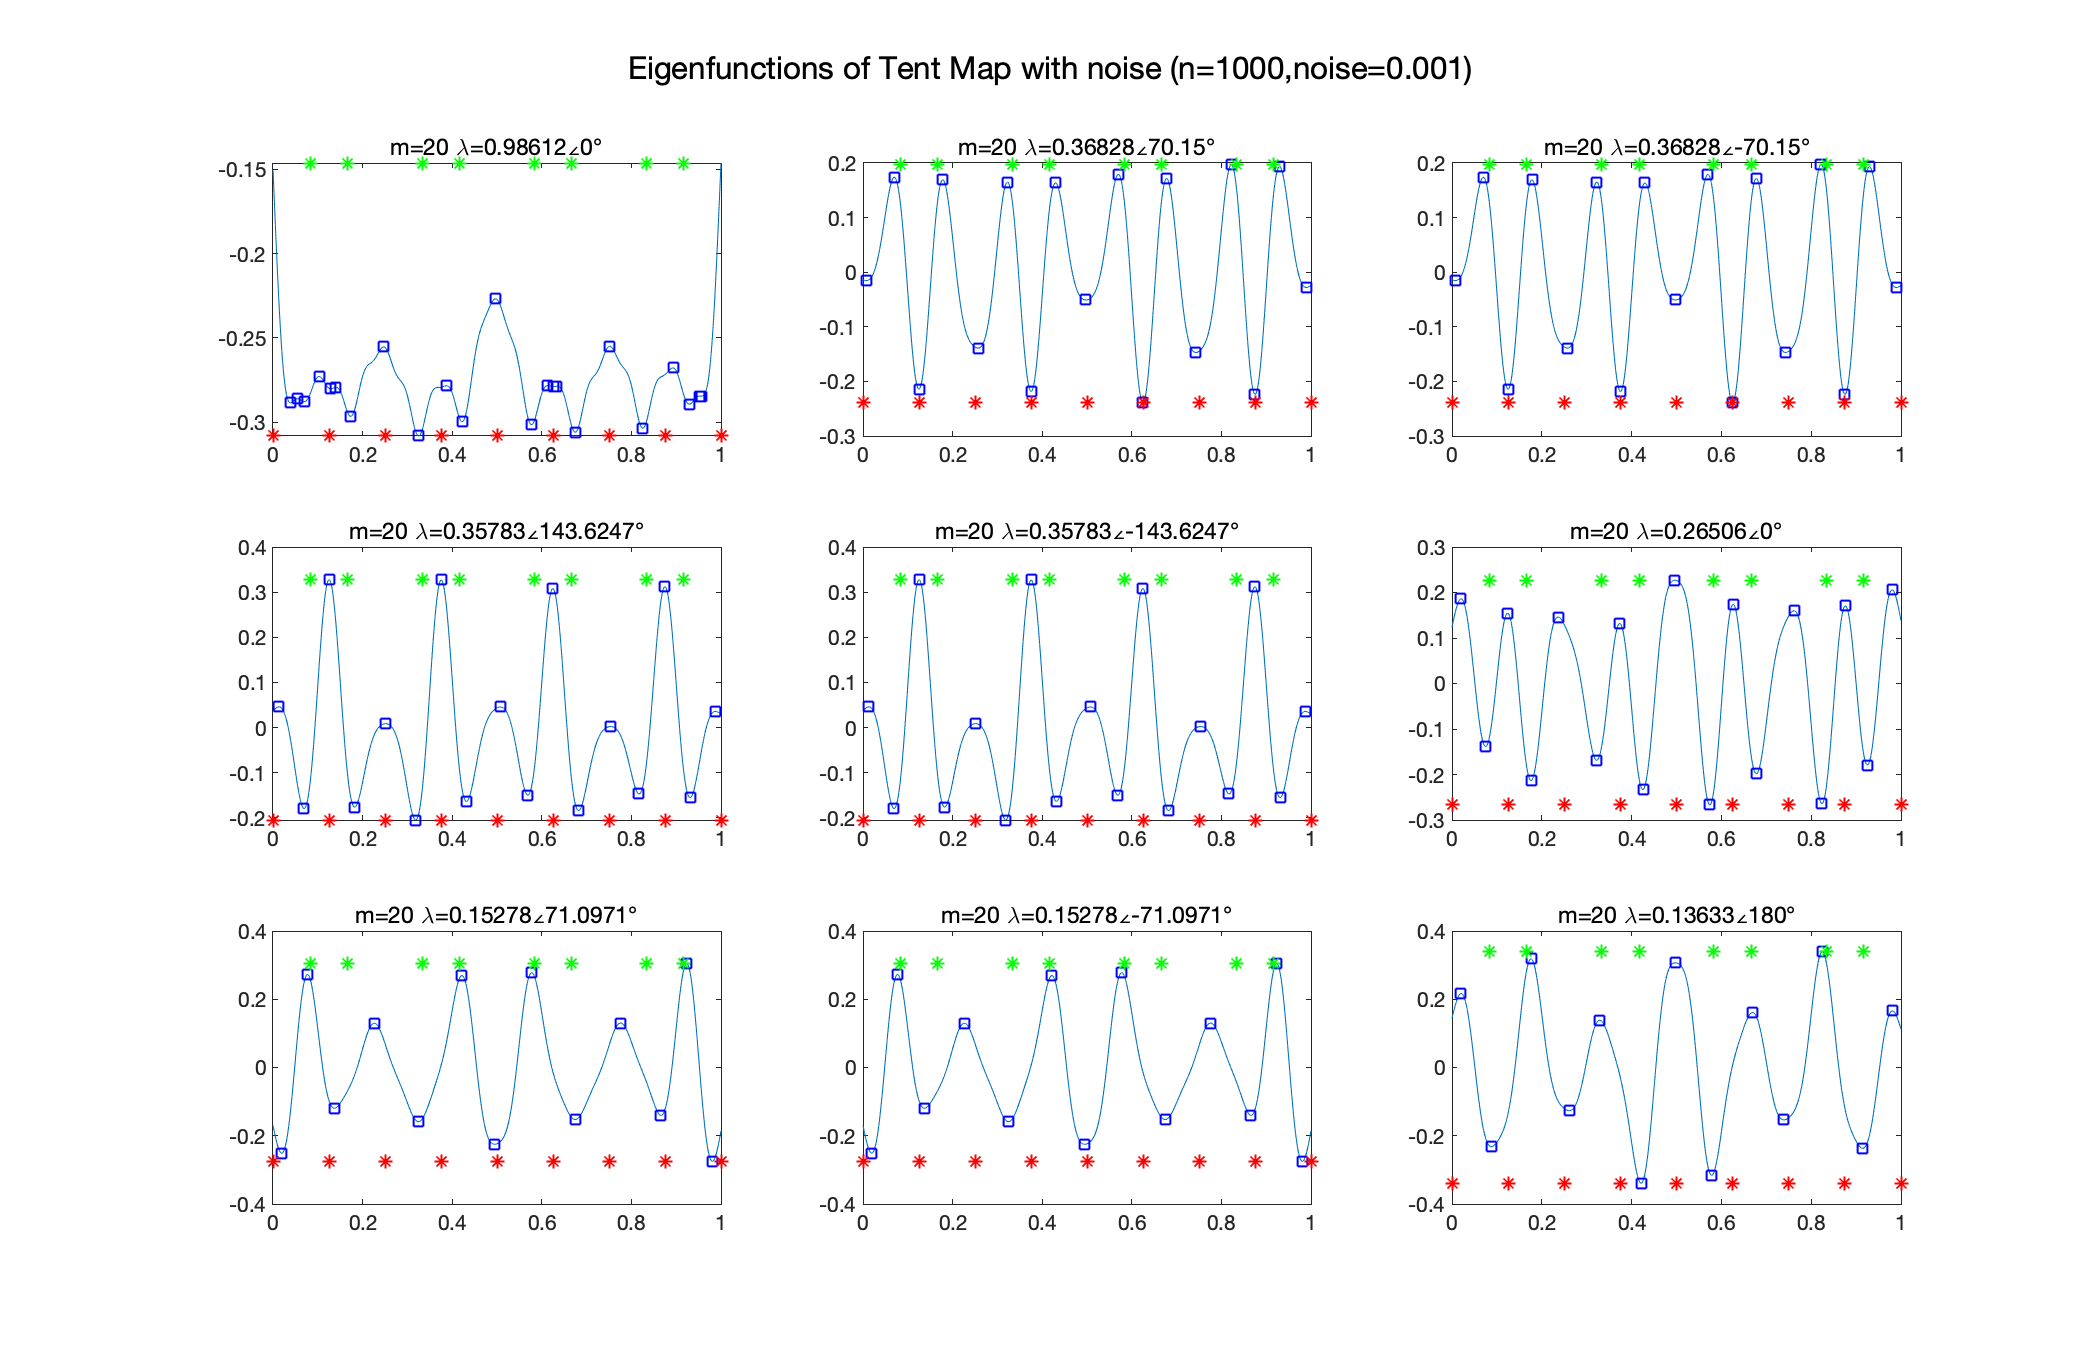
\includegraphics[scale=0.2]{tent/noise/Tent_eigen_noise_n1000m20d0-001}}
    \\
  \caption{帐篷映射的边界点与本征函数($noise=0.001$)}
\end{figure}

\begin{figure}
  \centering%[2,3,4,5,8,10,15,20]
  \subfloat[m=2]{
    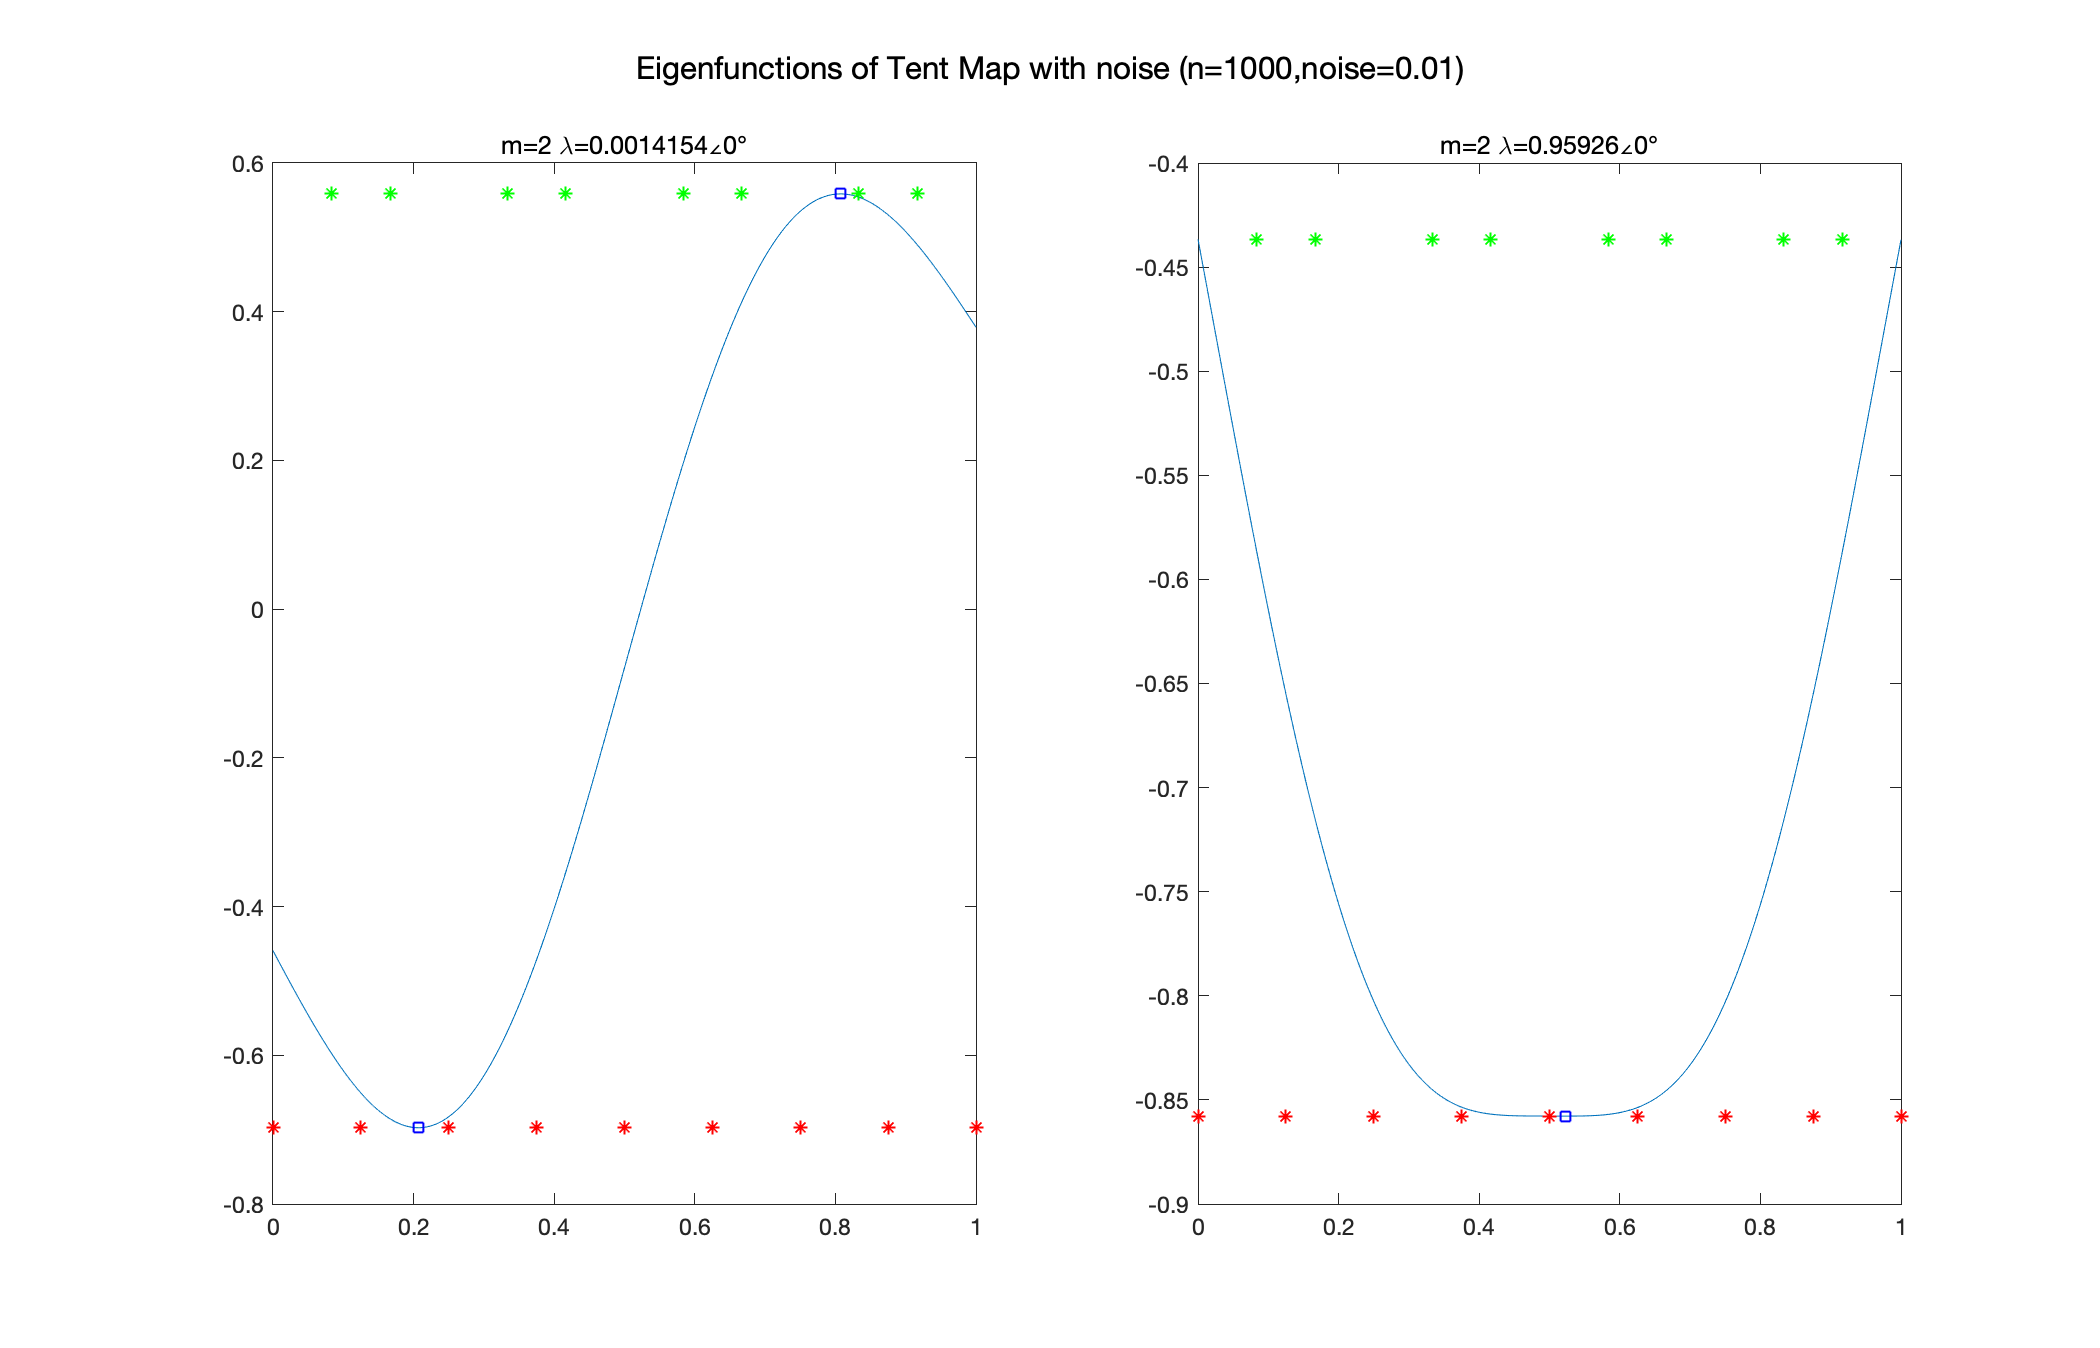
\includegraphics[scale=0.2]{tent/noise/Tent_eigen_noise_n1000m2d0-01}}
  \subfloat[m=3]{
    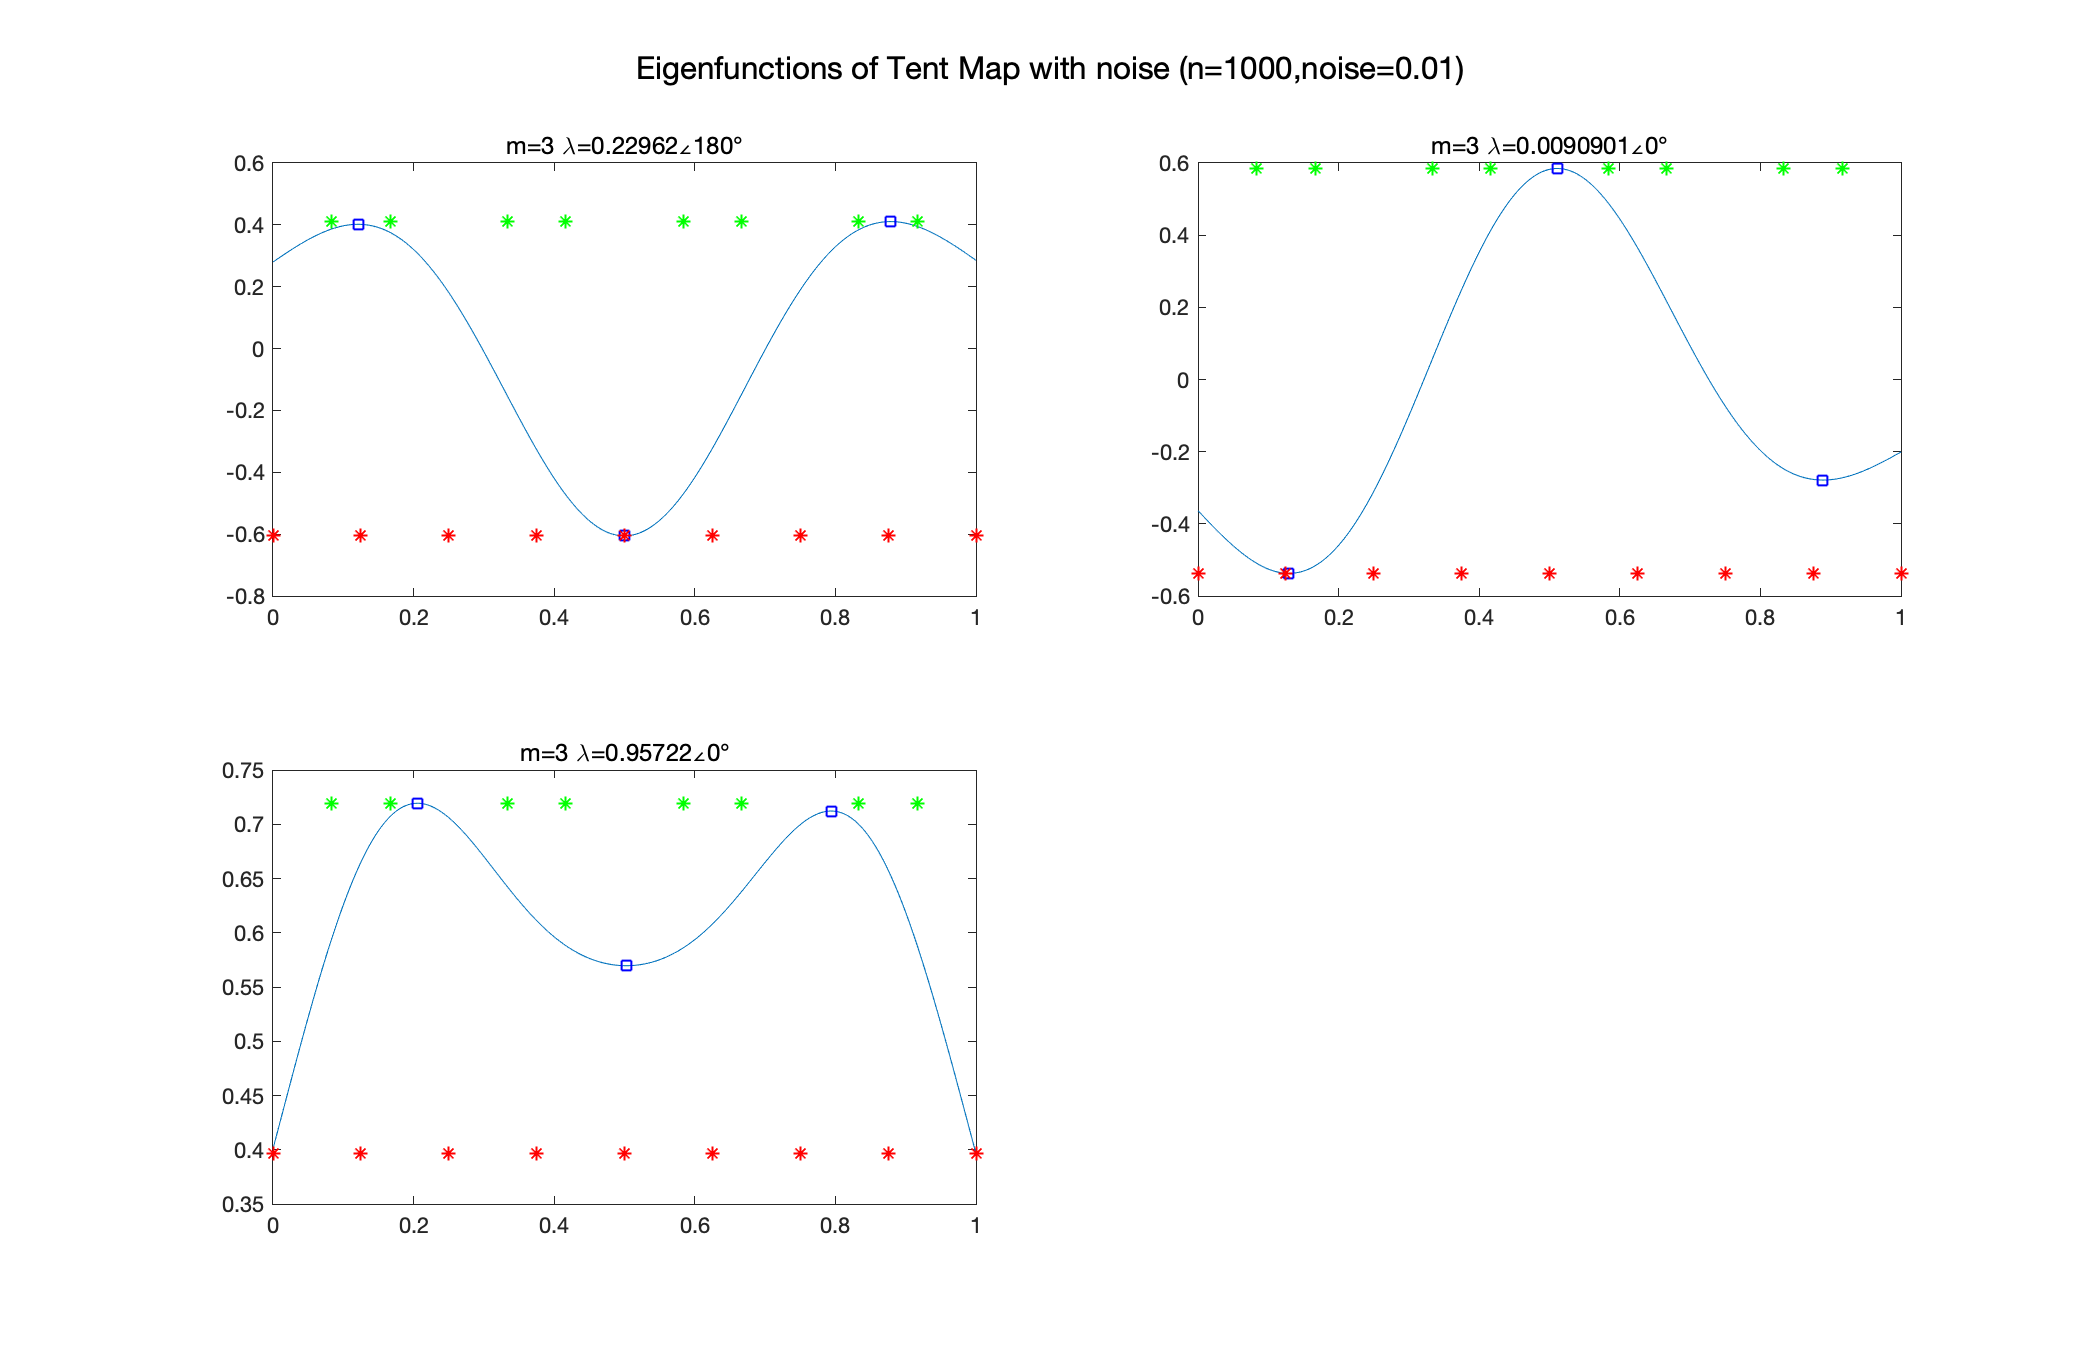
\includegraphics[scale=0.2]{tent/noise/Tent_eigen_noise_n1000m3d0-01}}
    \\
  \subfloat[m=4]{
    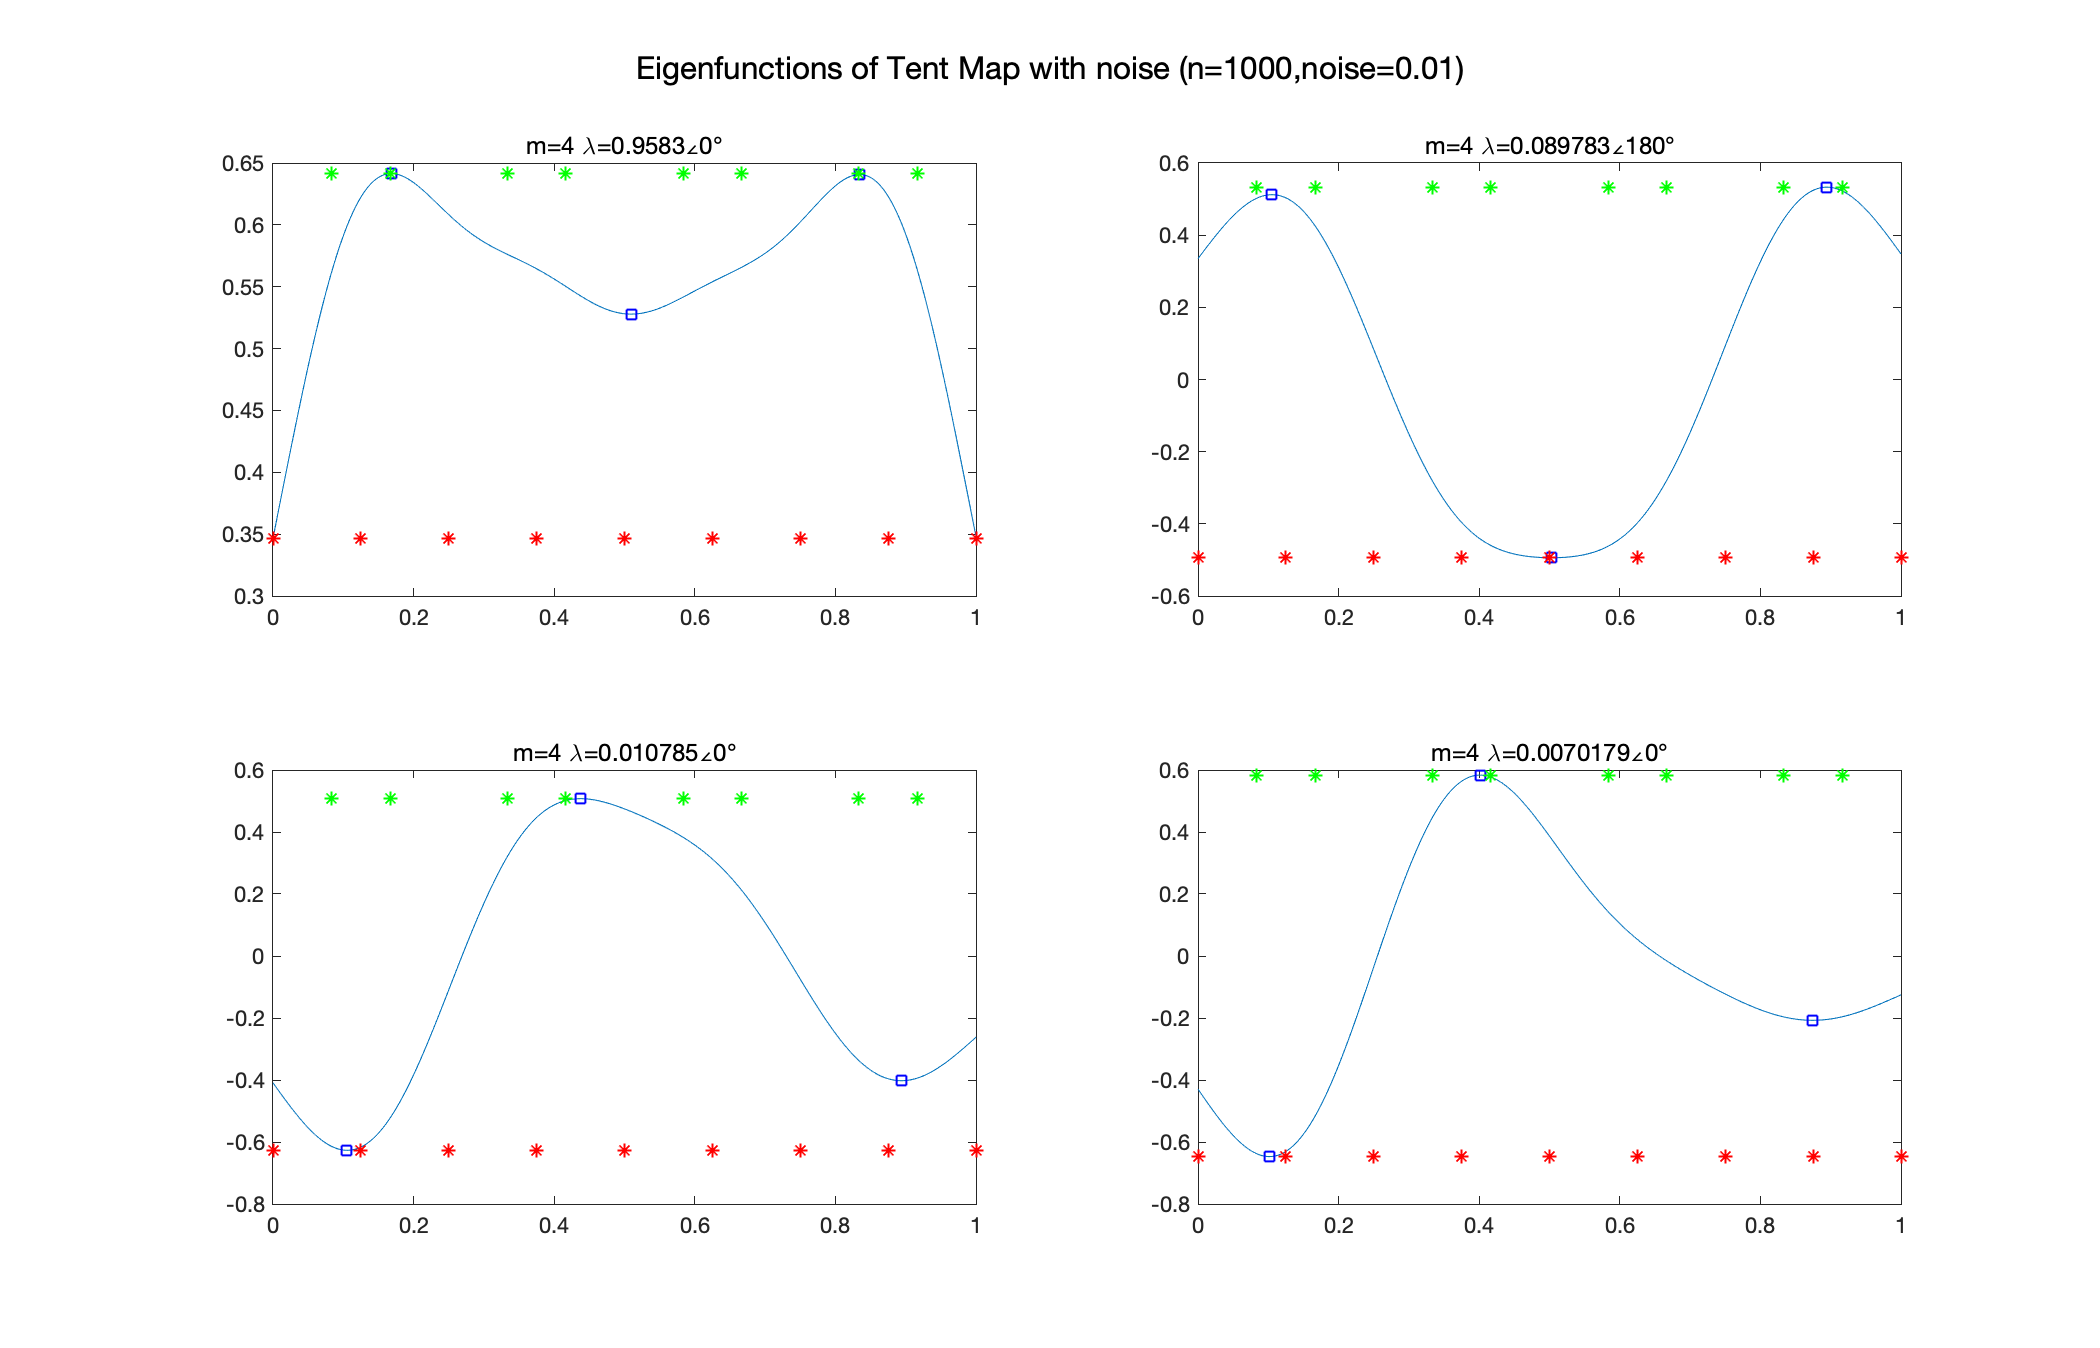
\includegraphics[scale=0.2]{tent/noise/Tent_eigen_noise_n1000m4d0-01}}
  \subfloat[m=5]{
    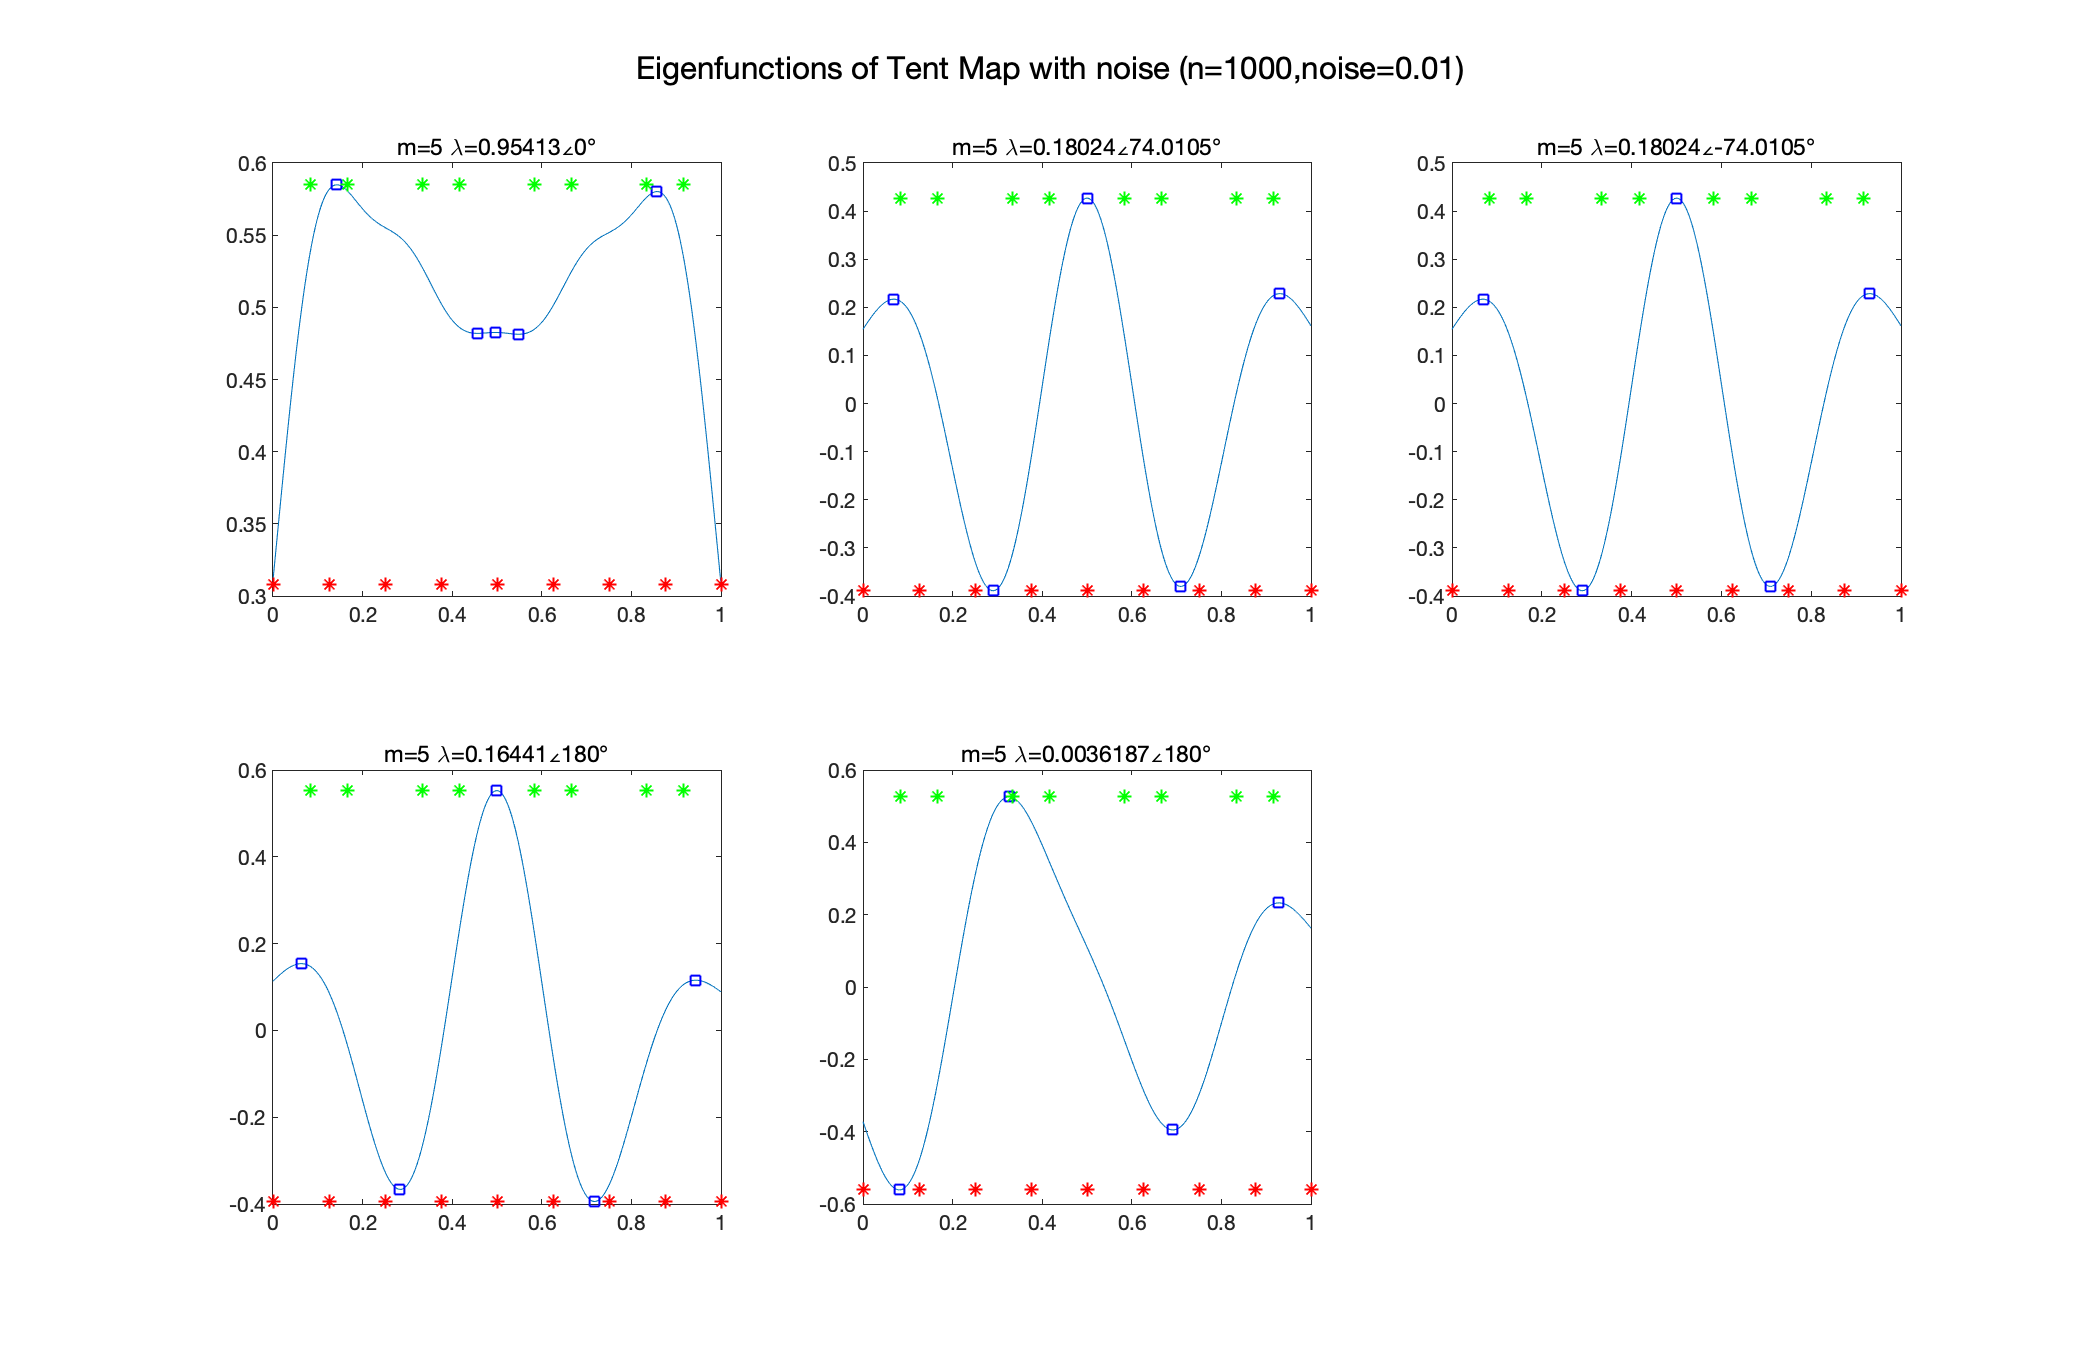
\includegraphics[scale=0.2]{tent/noise/Tent_eigen_noise_n1000m5d0-01}}
    \\
  \subfloat[m=8]{
    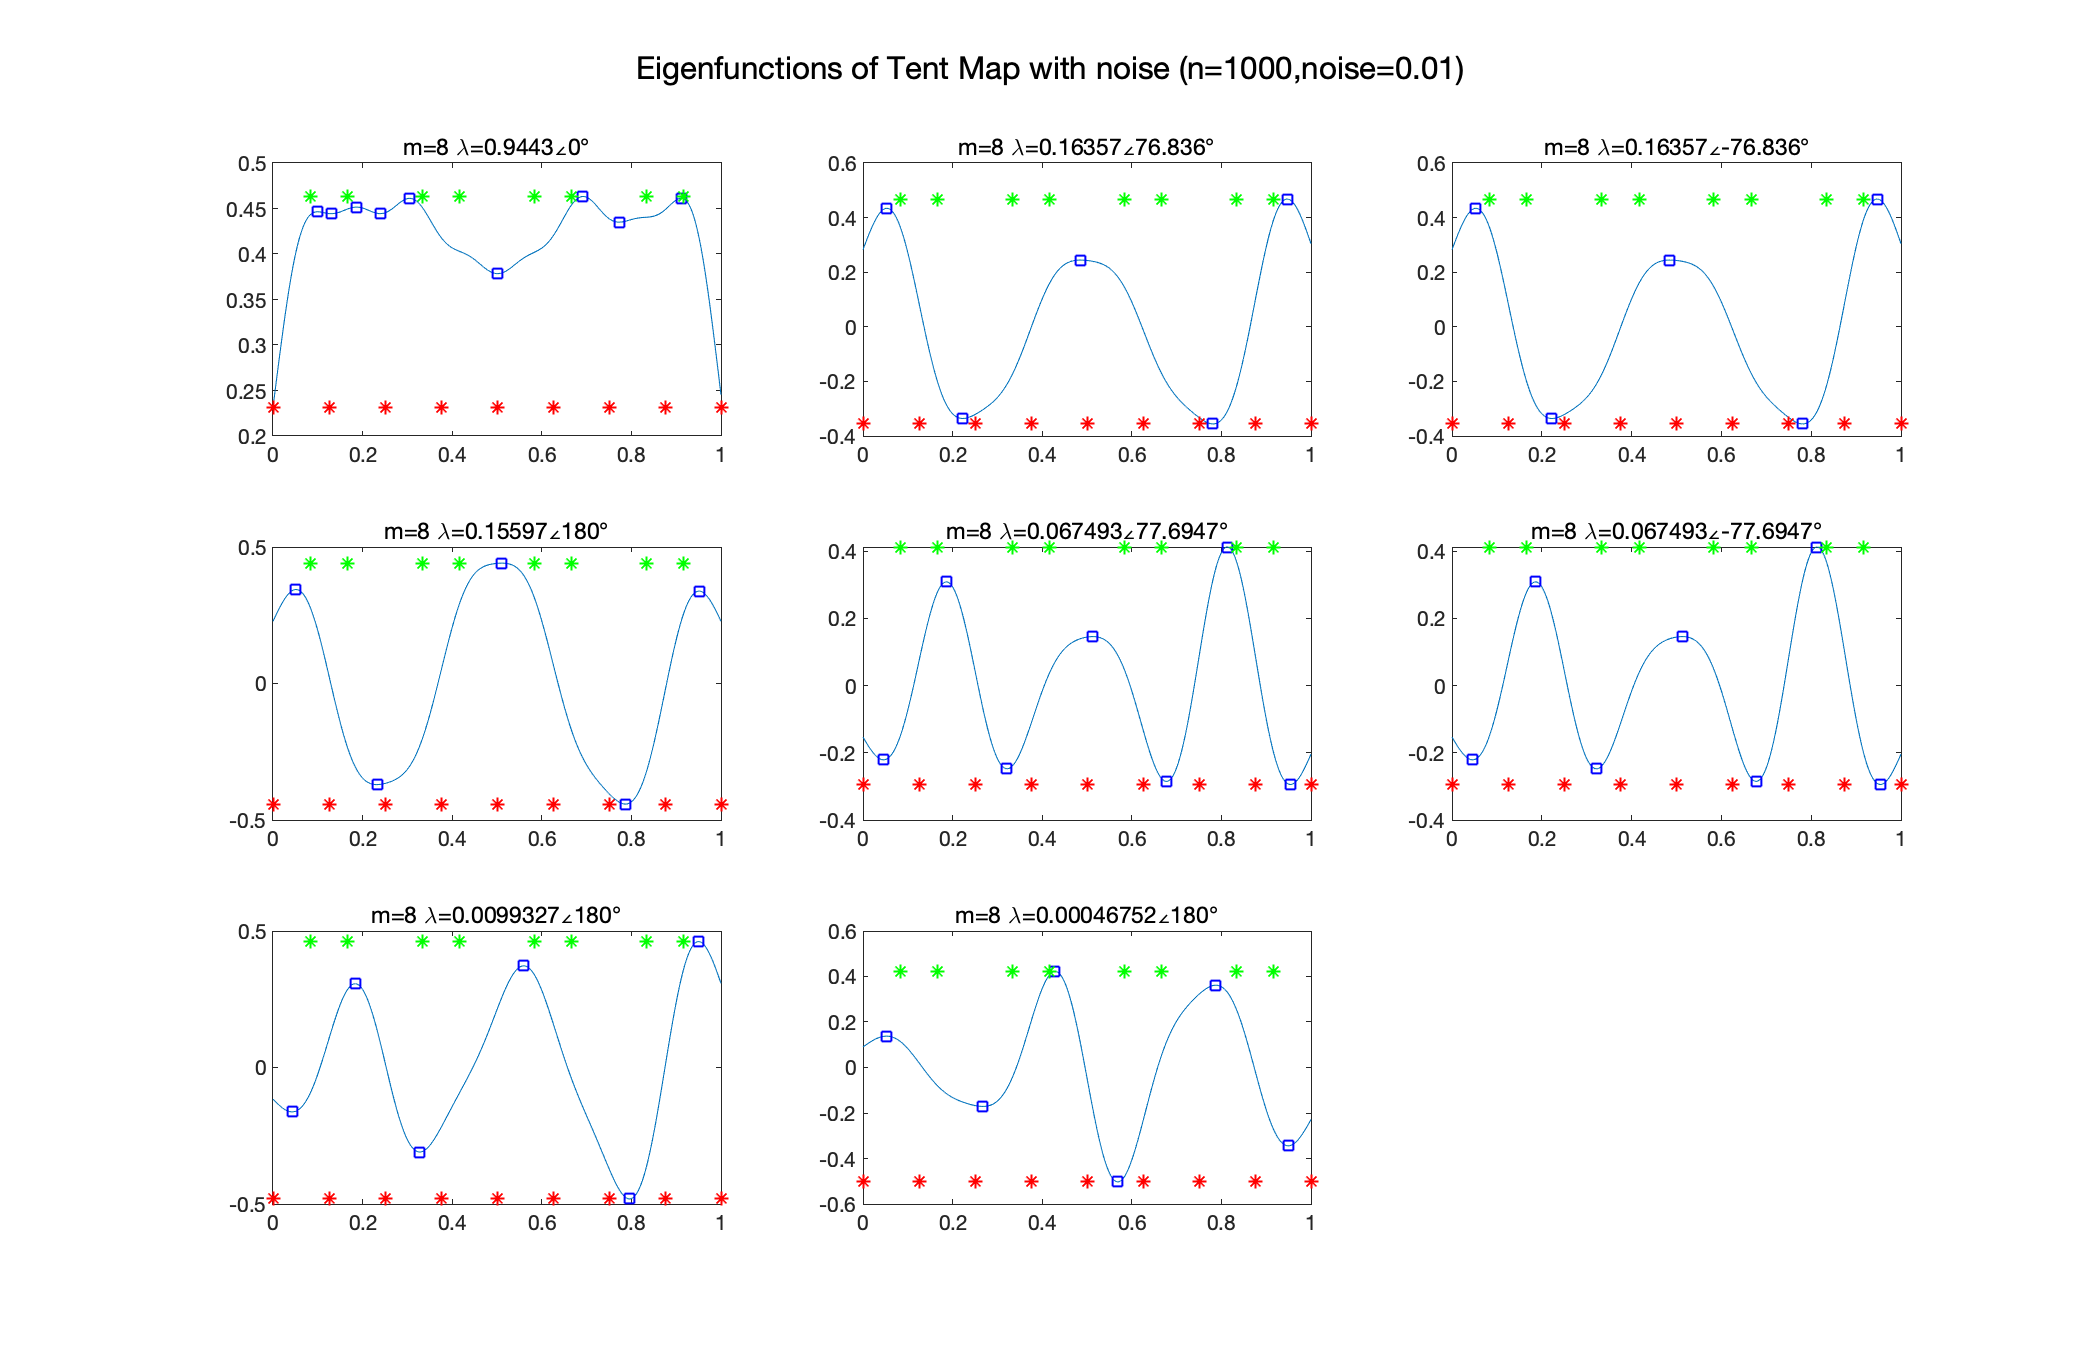
\includegraphics[scale=0.2]{tent/noise/Tent_eigen_noise_n1000m8d0-01}}
  \subfloat[m=10]{
    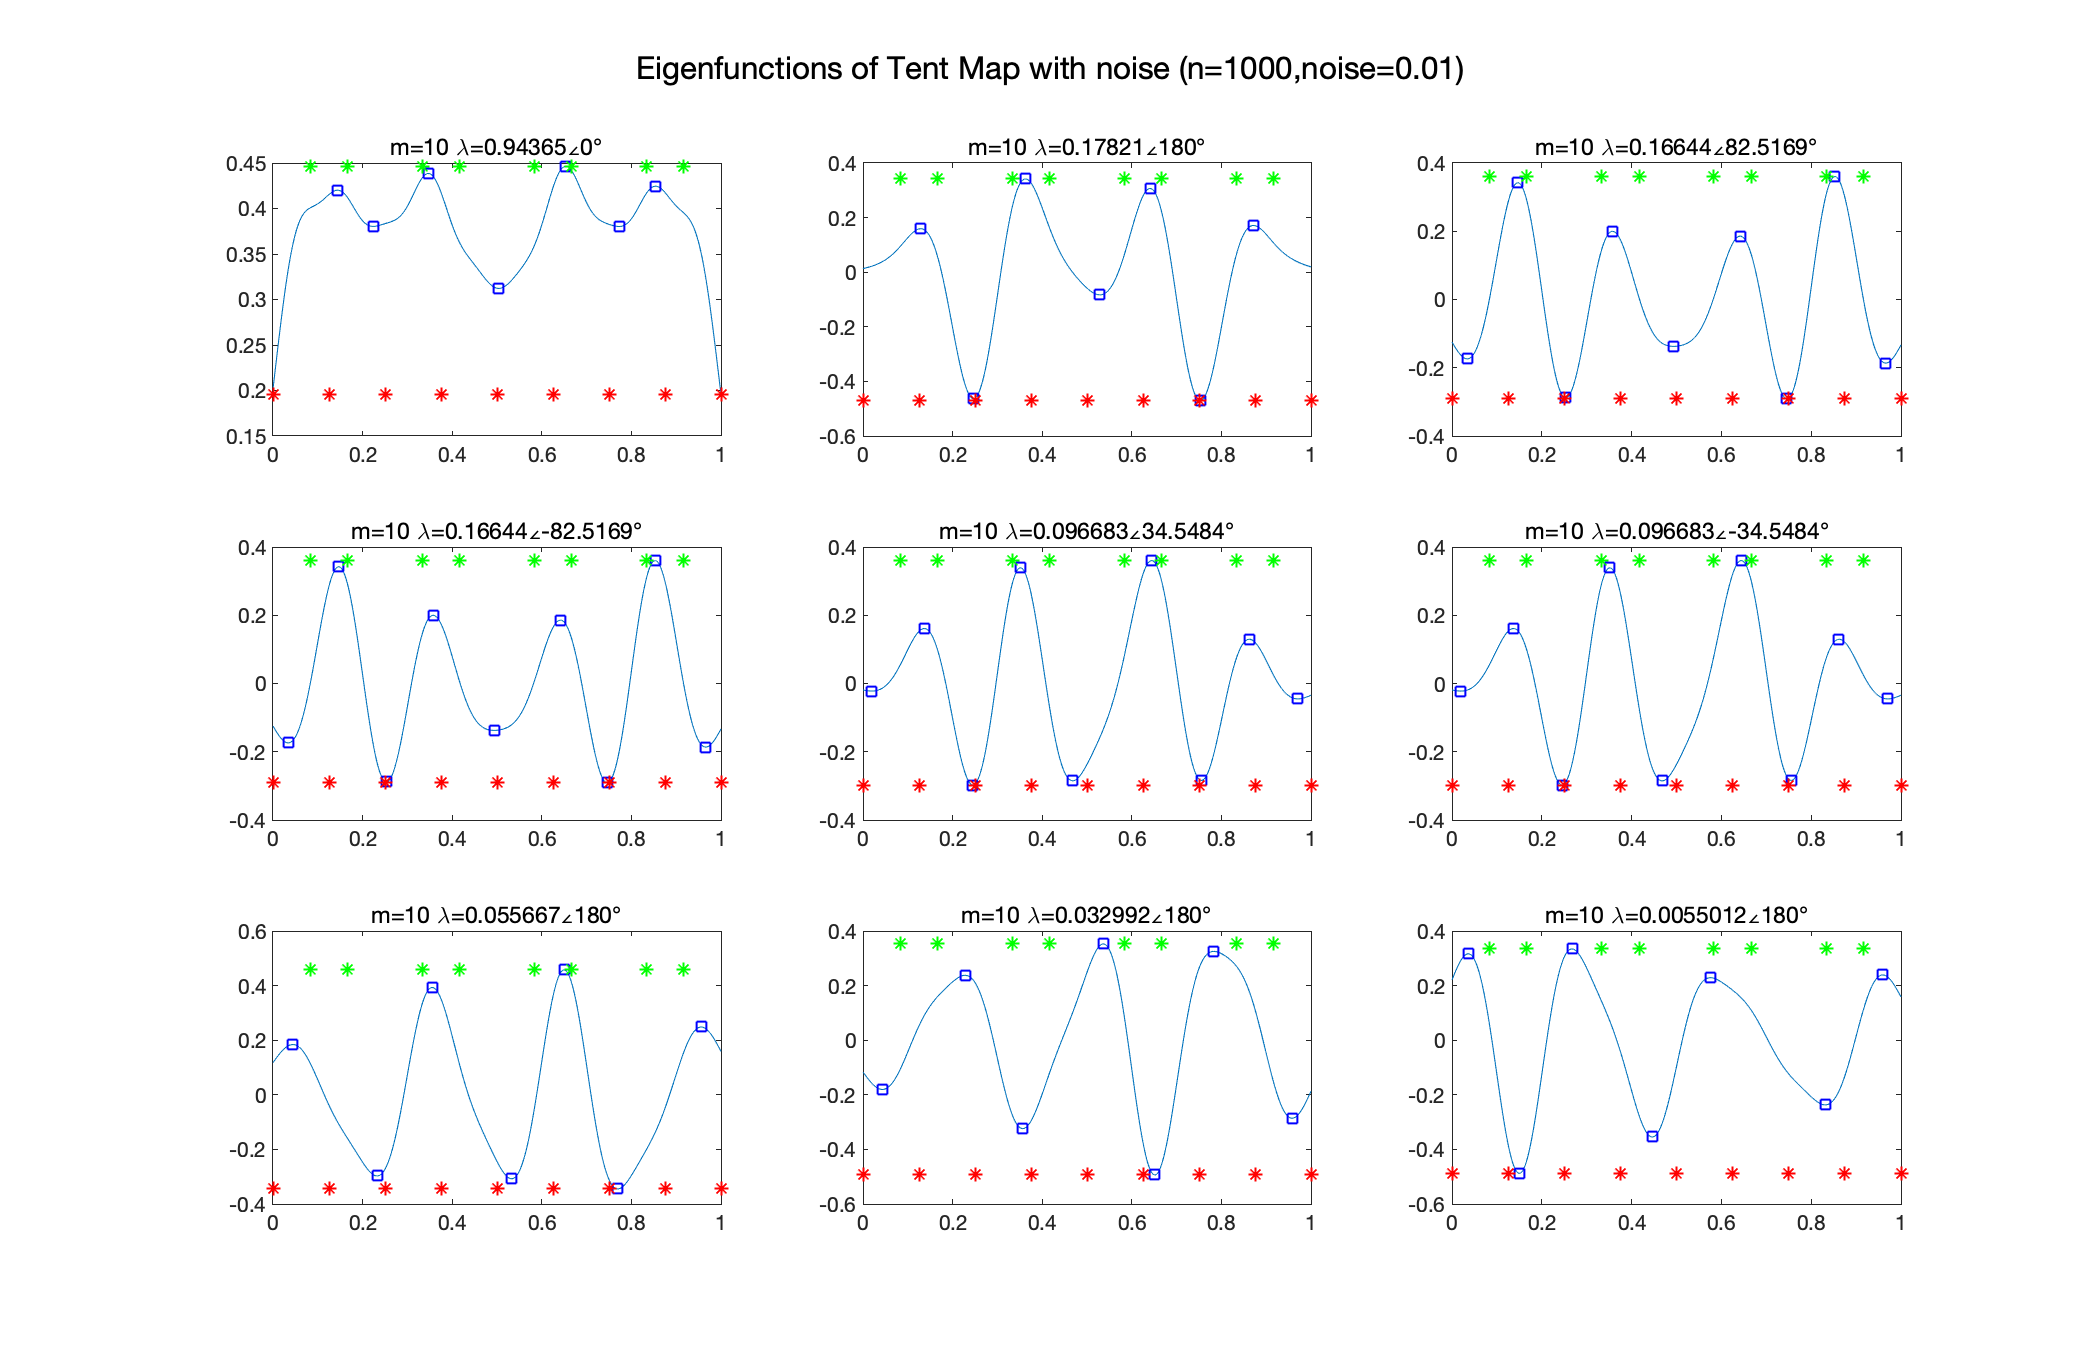
\includegraphics[scale=0.2]{tent/noise/Tent_eigen_noise_n1000m10d0-01}}
    \\
  \subfloat[m=15]{
    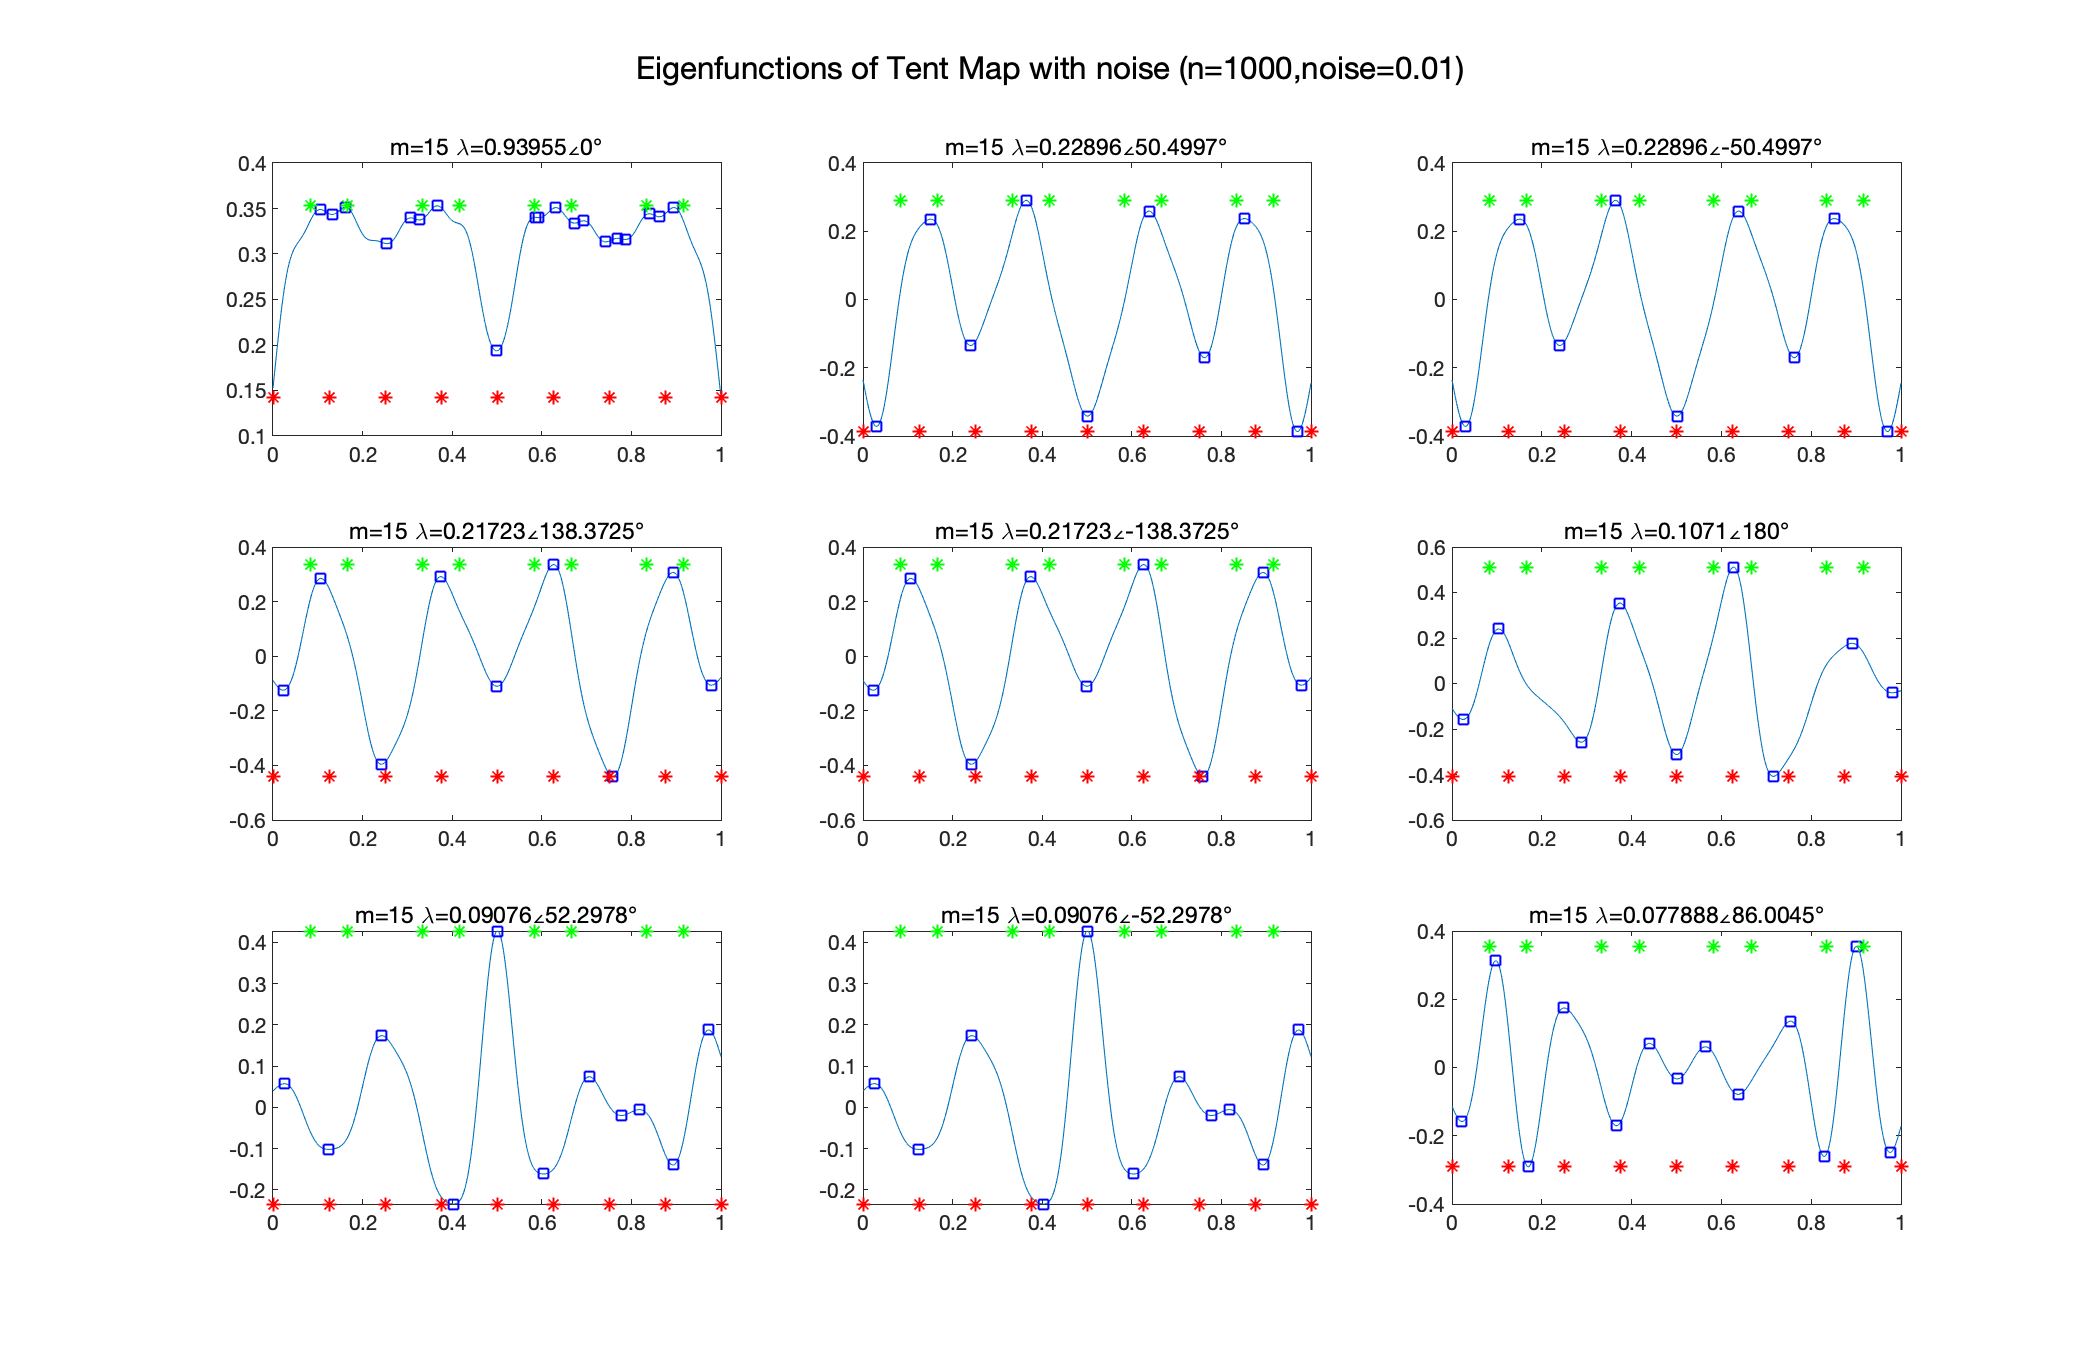
\includegraphics[scale=0.2]{tent/noise/Tent_eigen_noise_n1000m15d0-01}}
  \subfloat[m=20]{
    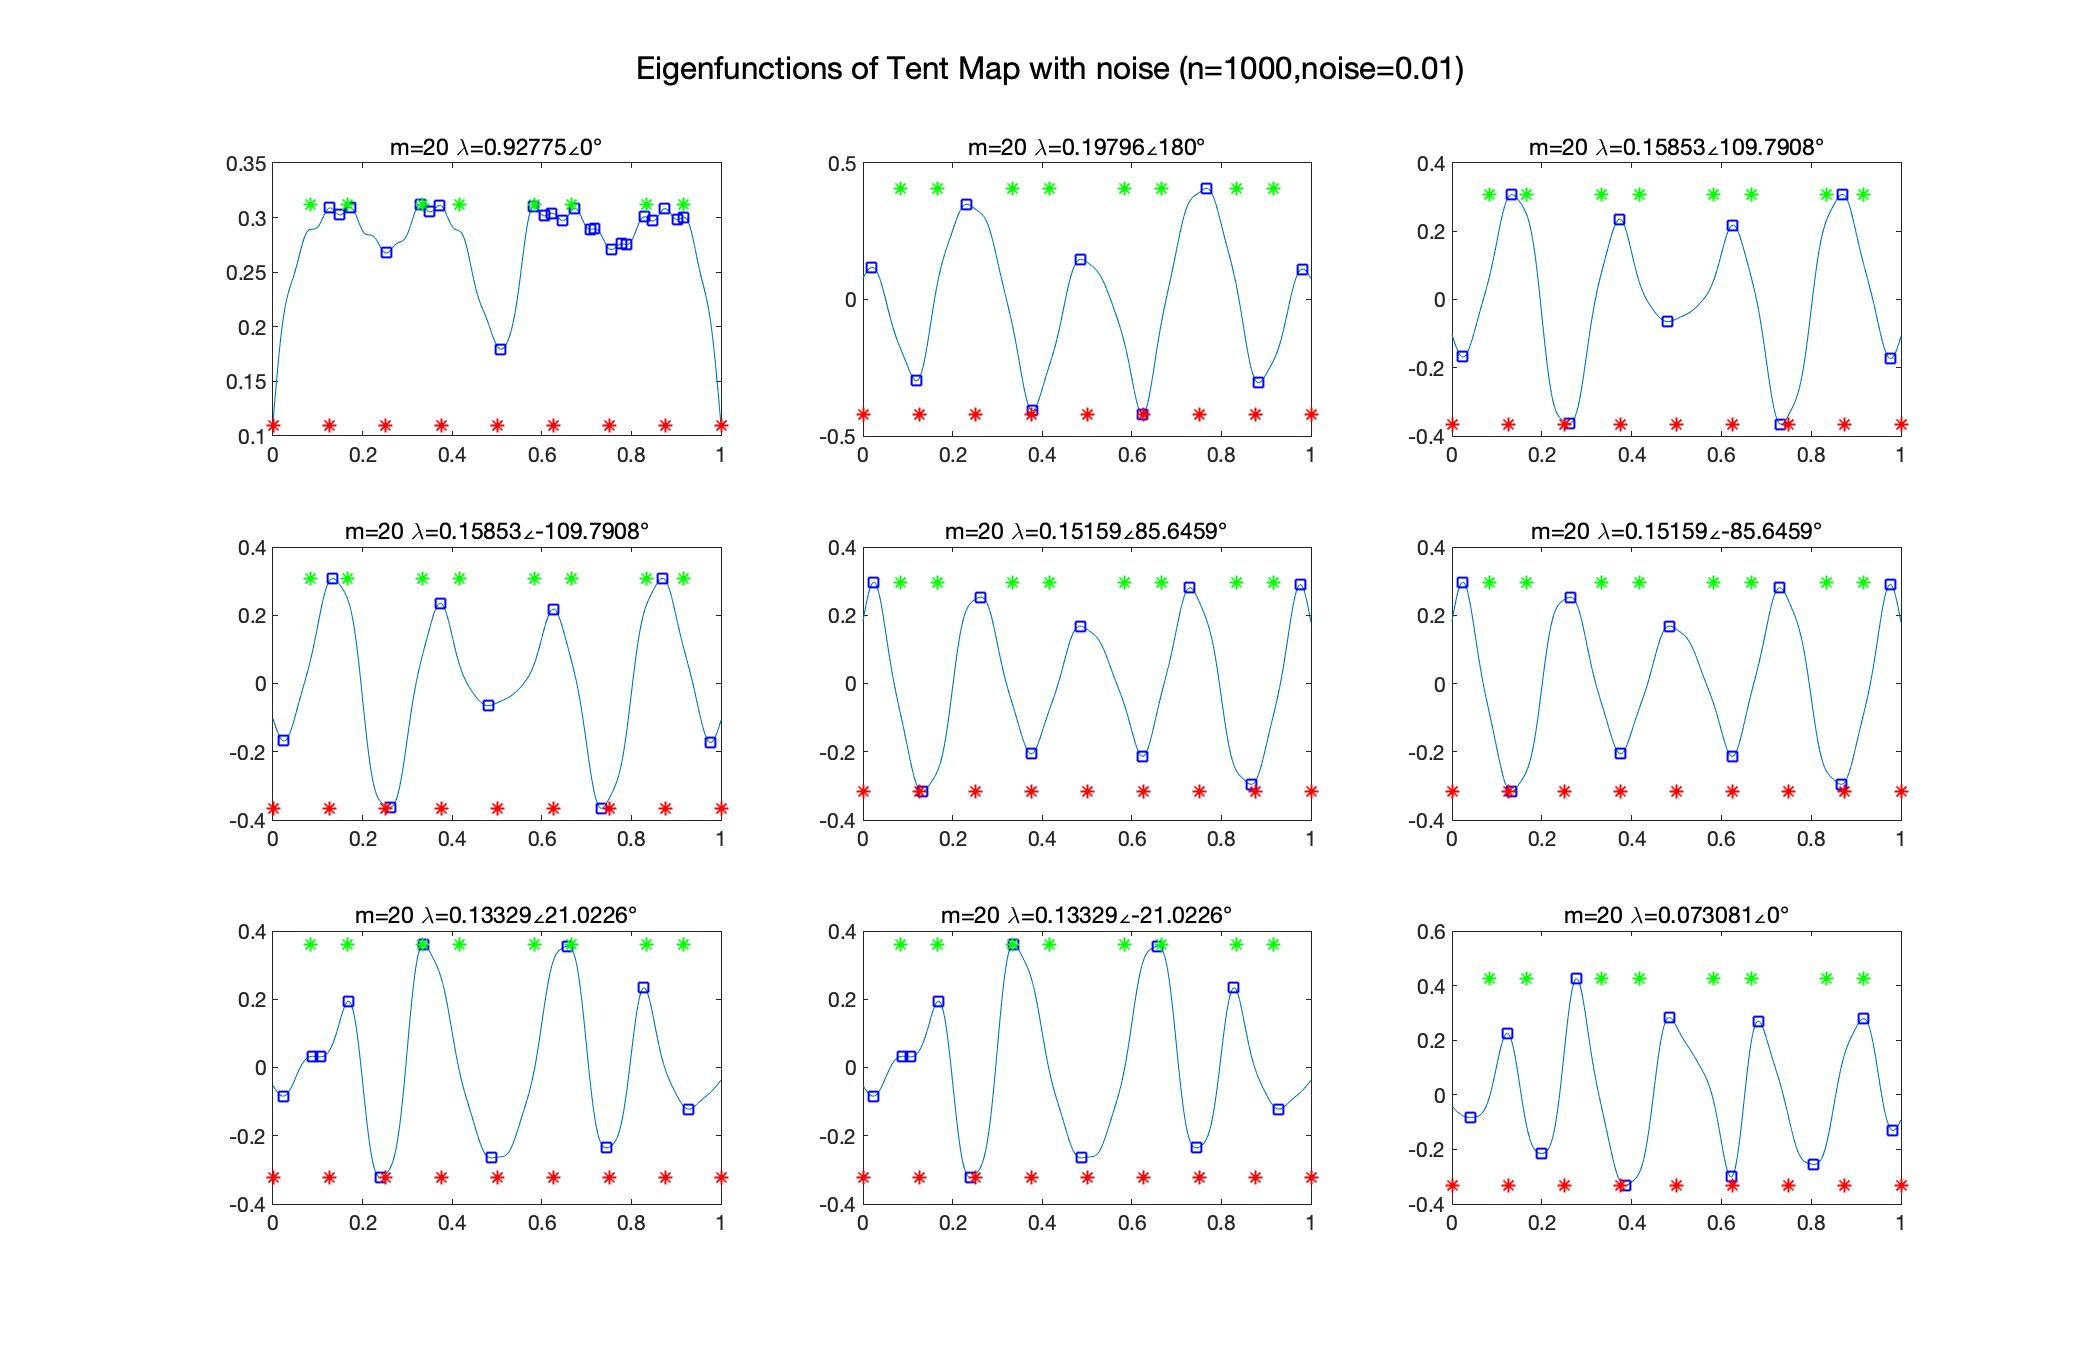
\includegraphics[scale=0.2]{tent/noise/Tent_eigen_noise_n1000m20d0-01}}
    \\
    \caption{帐篷映射的边界点与本征函数($noise=0.01$)}
\end{figure}
\subsubsection{寻找更精确的边界点}

\begin{figure}
  \centering
  \subfloat[m=8,16]{
    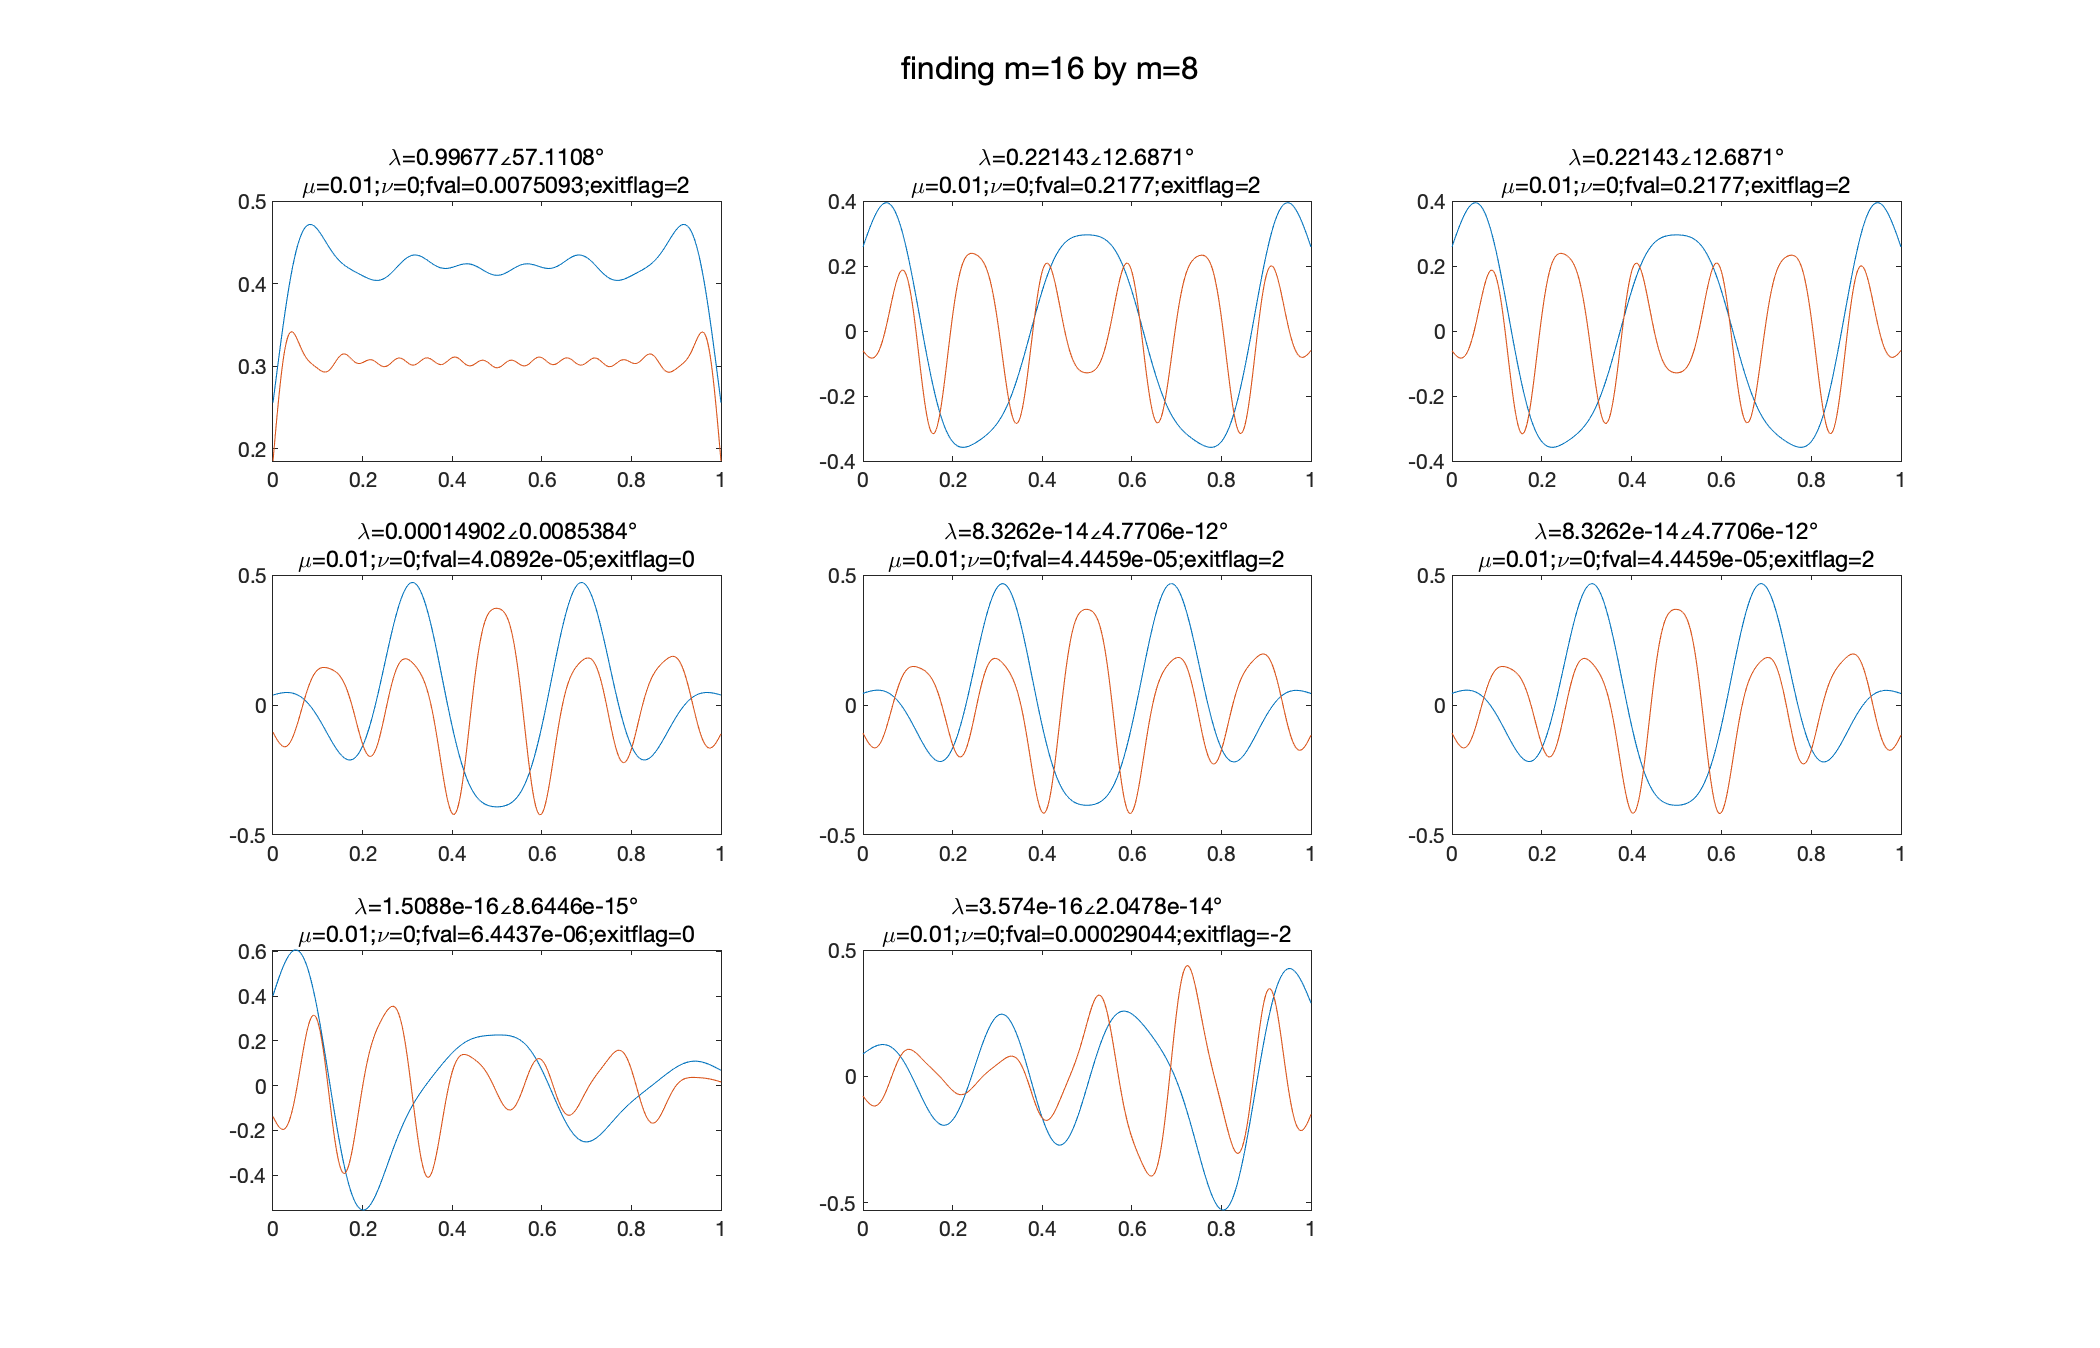
\includegraphics[scale=0.2]{tent/accurate/Tent_findeigen_m8m16}}
  \subfloat[m=16,32]{
    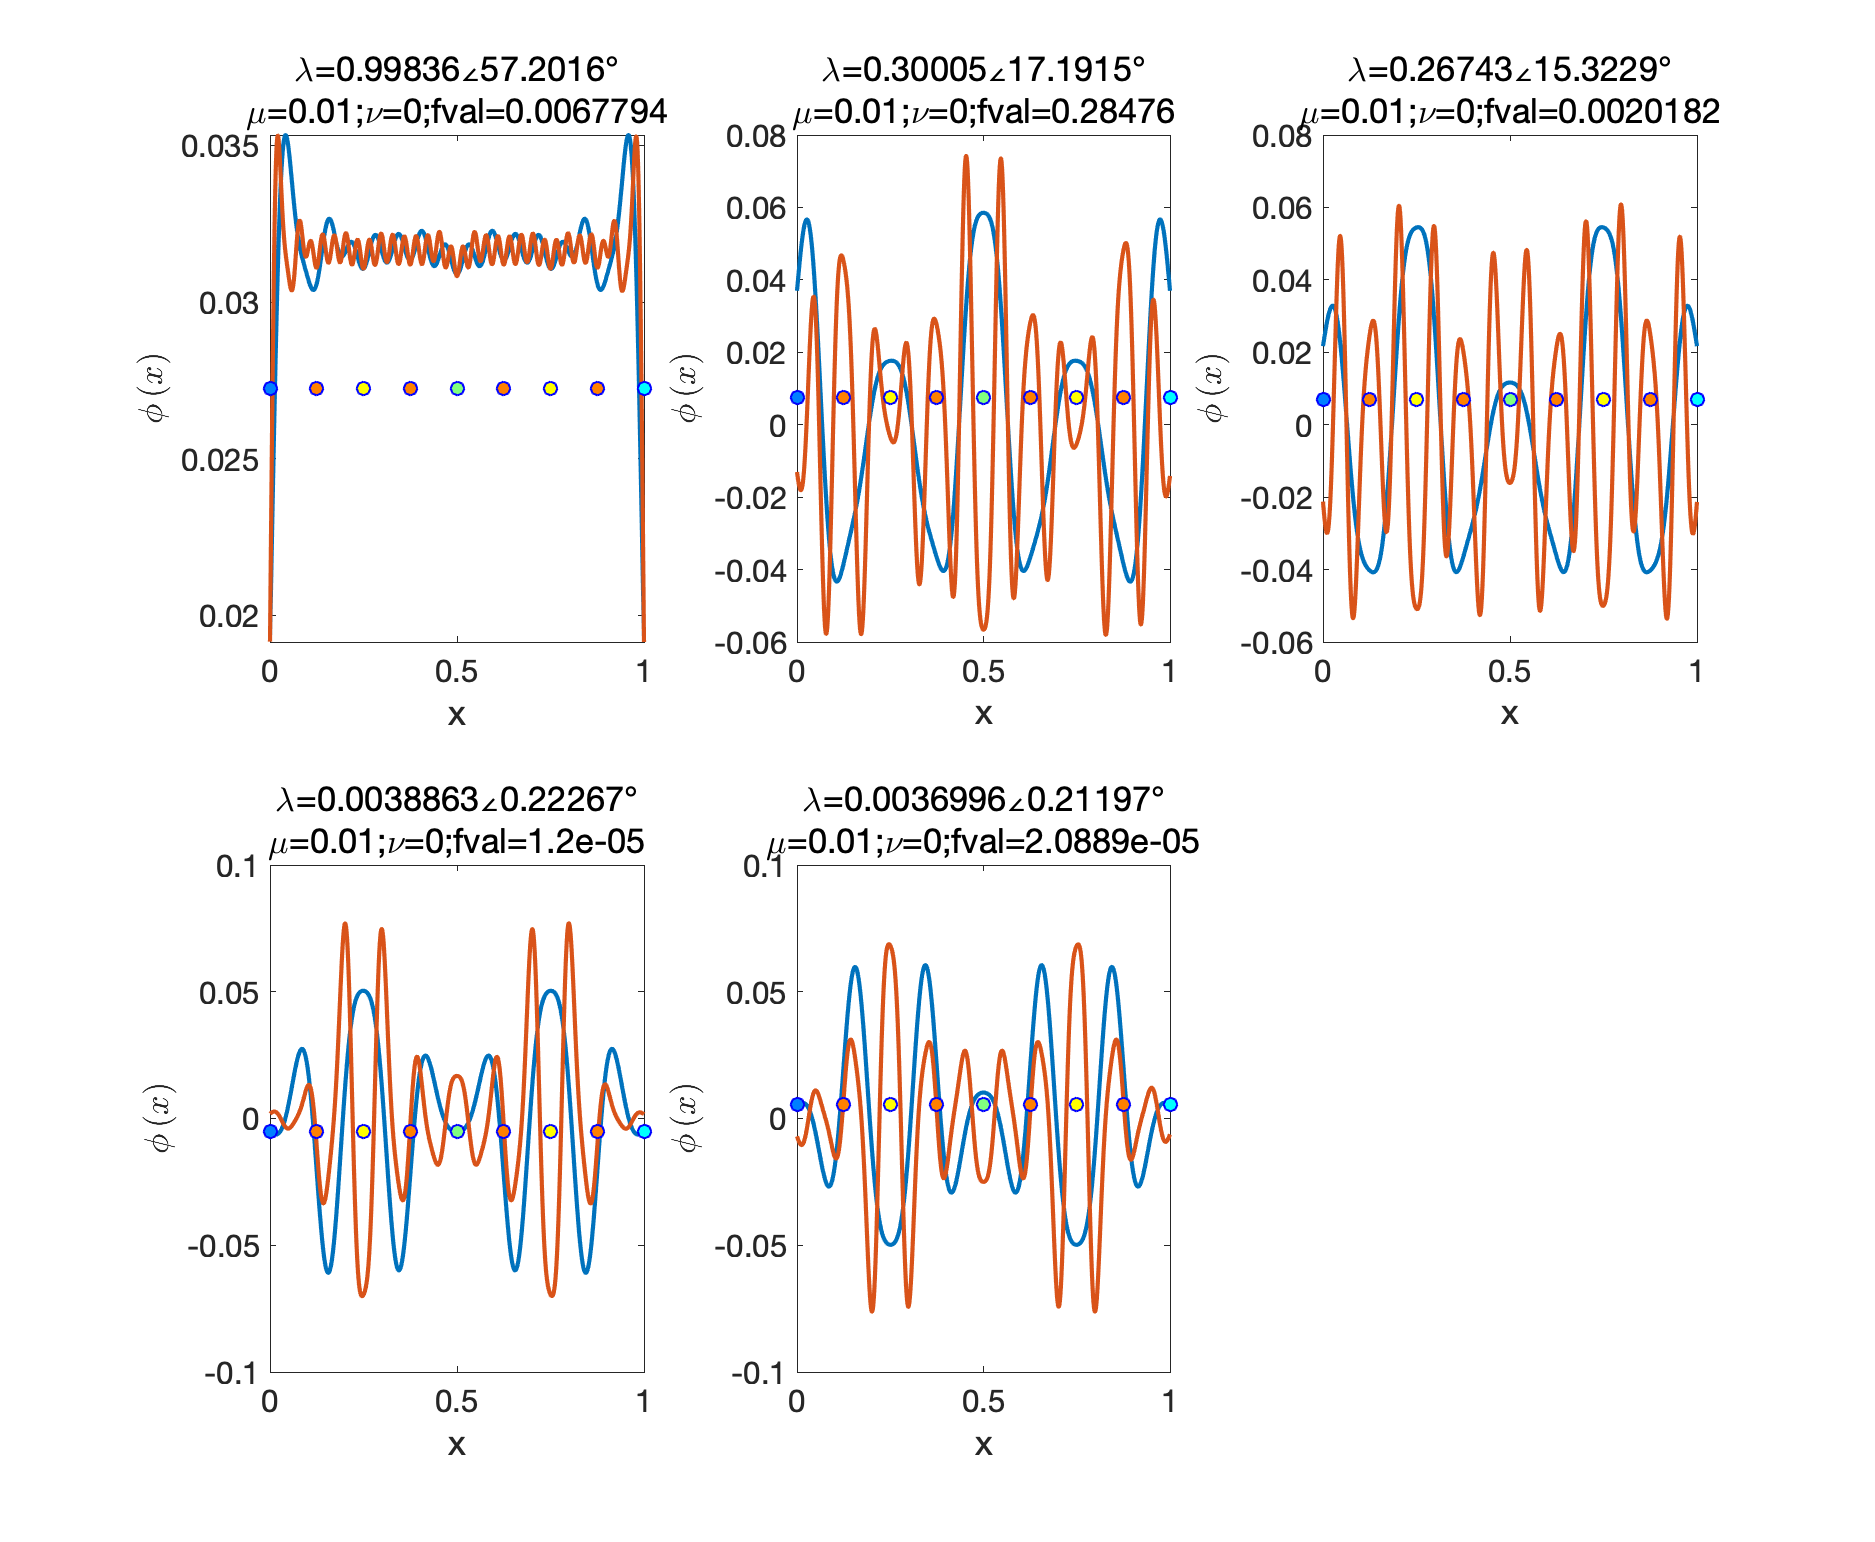
\includegraphics[scale=0.2]{tent/accurate/Tent_findeigen_m16m32}}
    \\
  \subfloat[m=32,64]{
    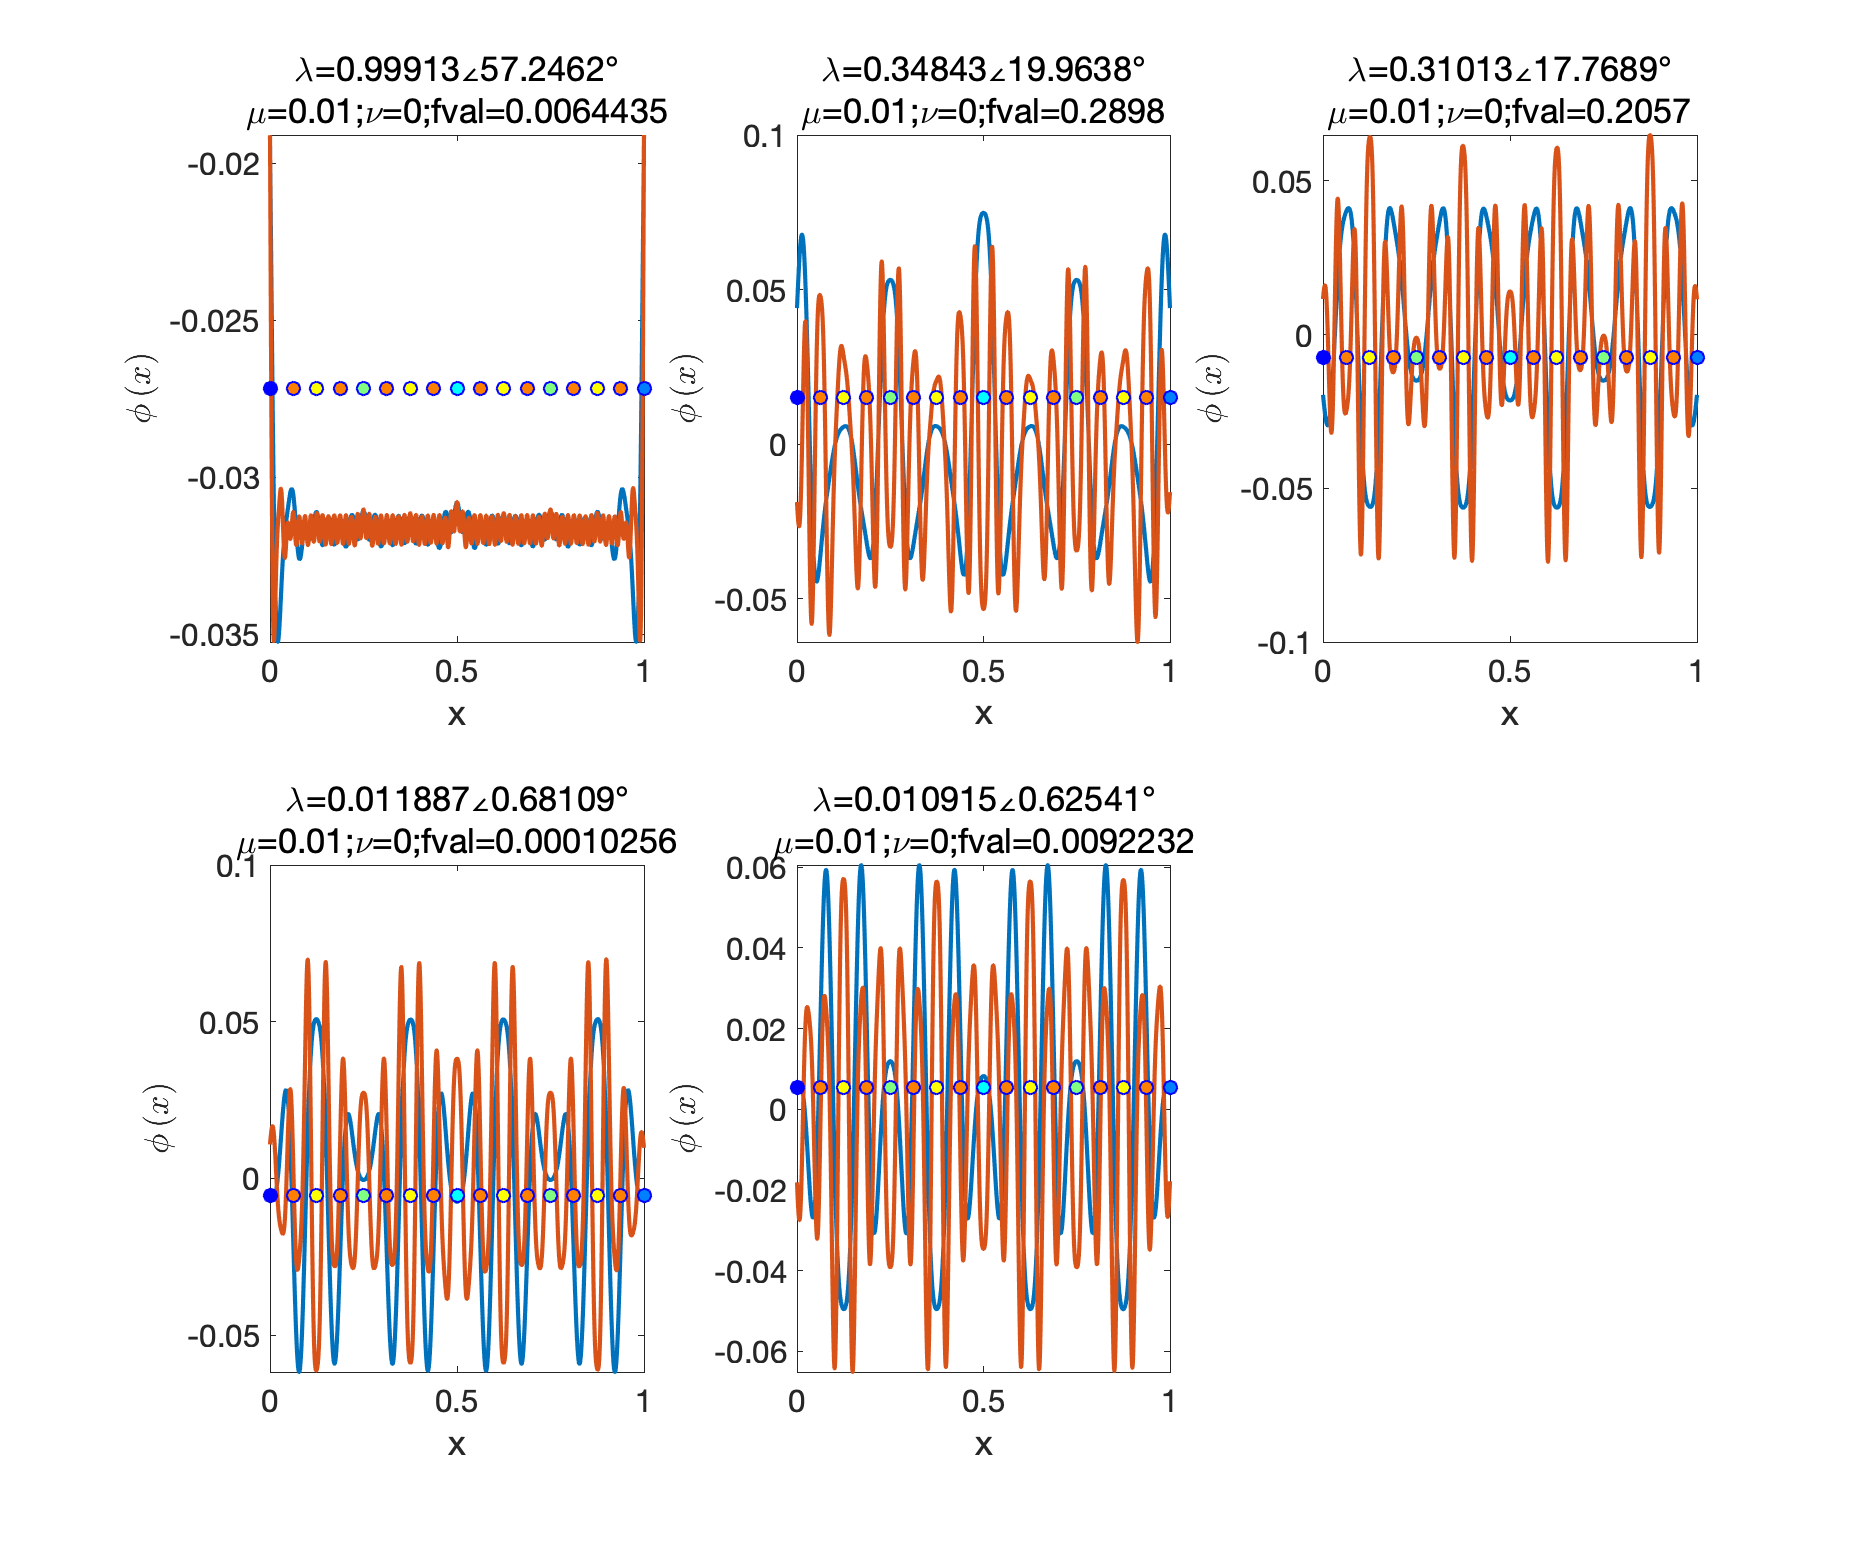
\includegraphics[scale=0.2]{tent/accurate/Tent_findeigen_m32m64}}
  \subfloat[m=64,128]{
    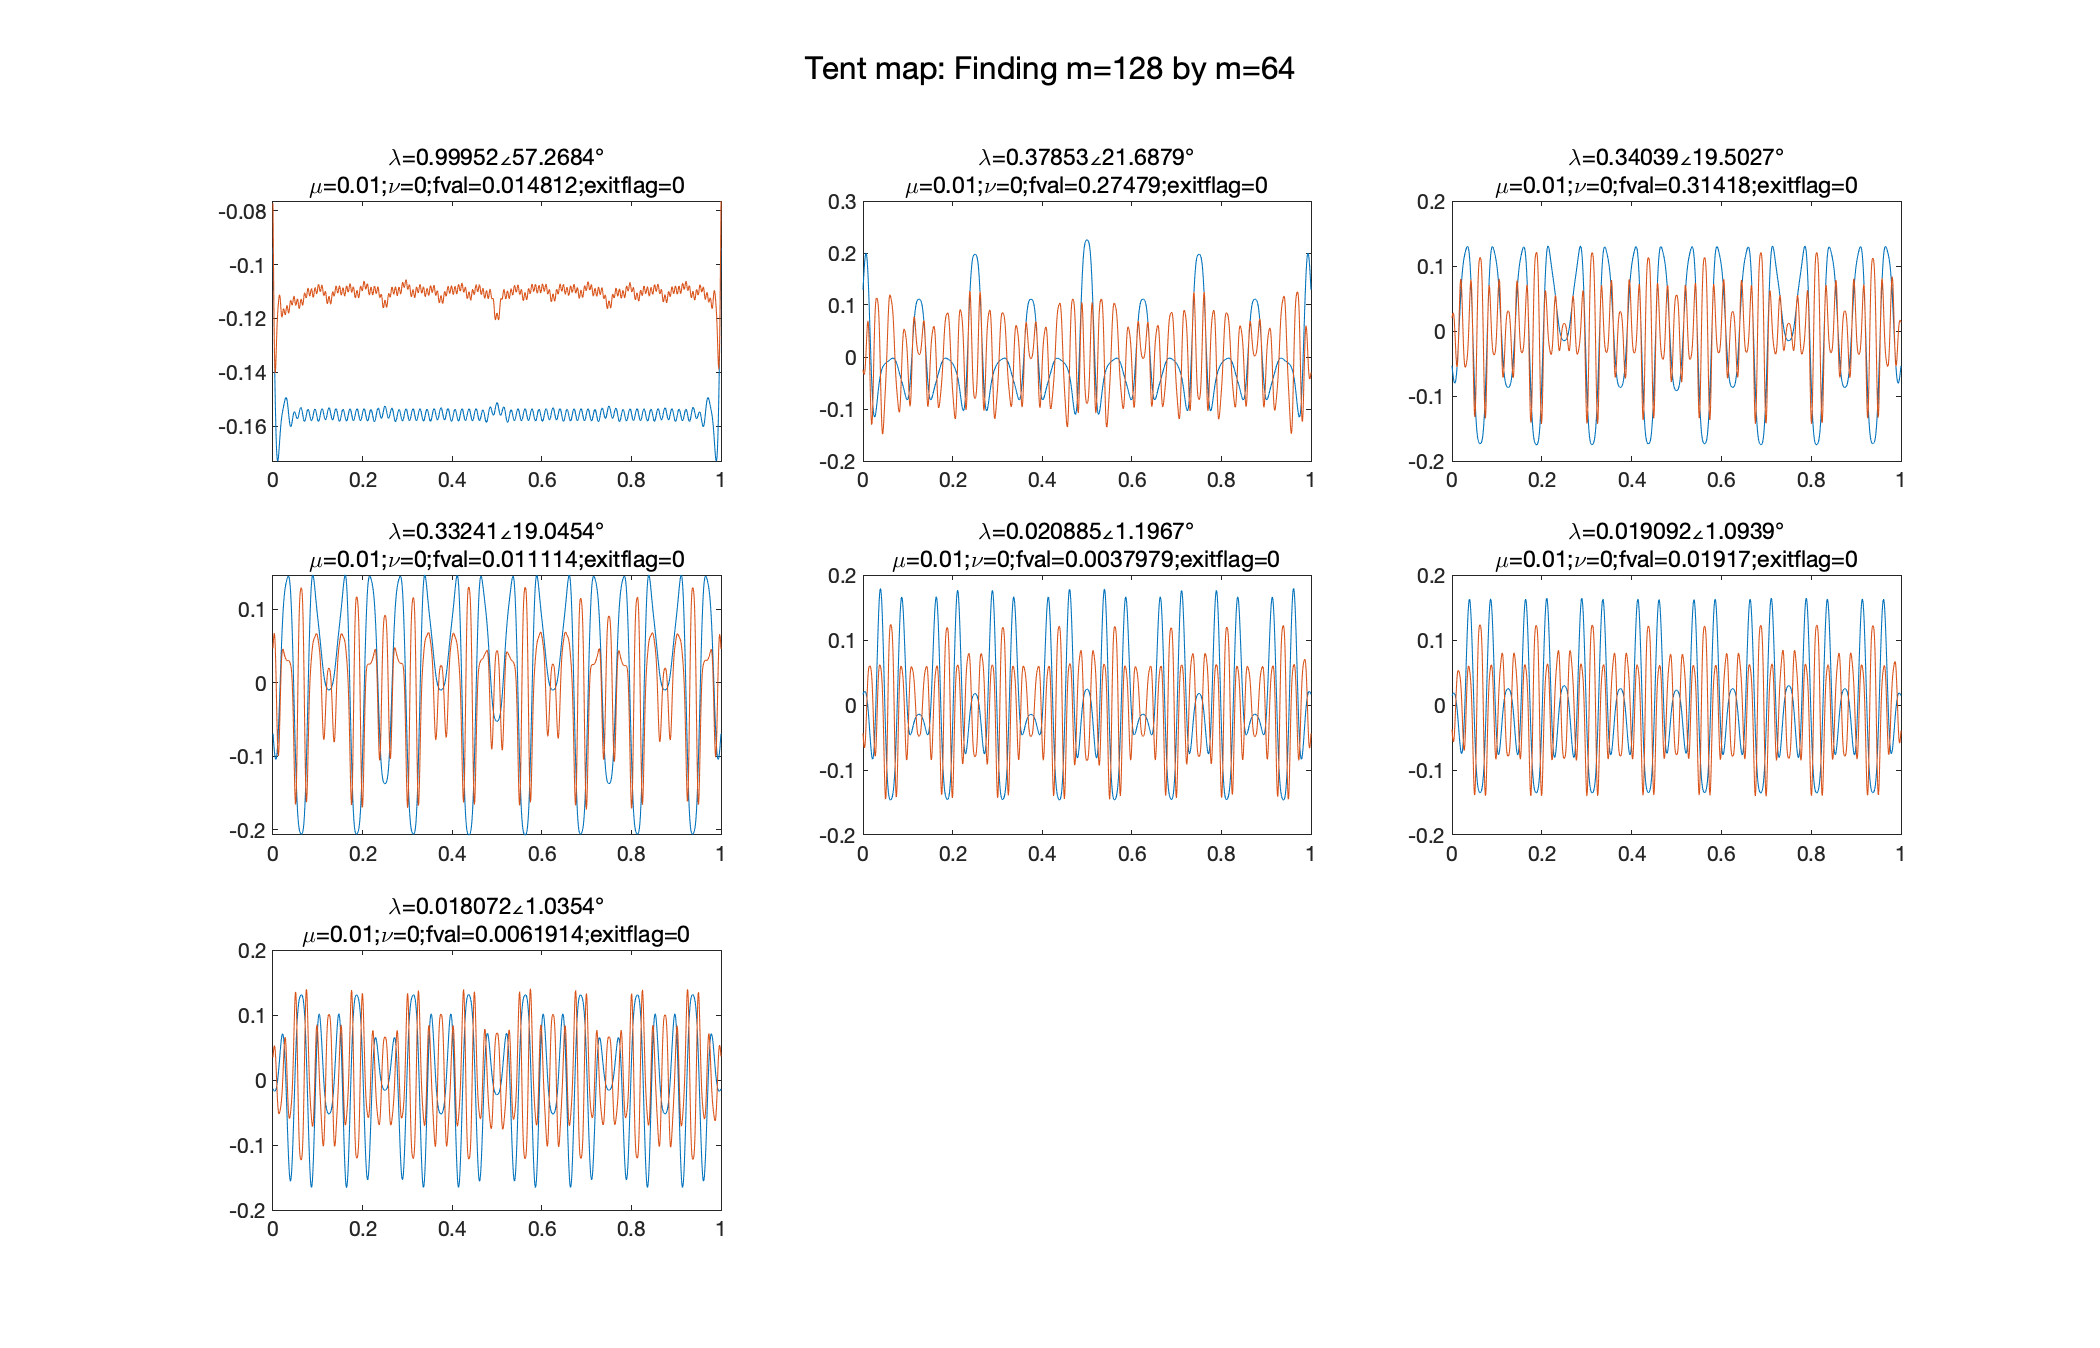
\includegraphics[scale=0.2]{tent/accurate/Tent_findeigen_m64m128}}
    \\
  \caption{帐篷映射本征函数不同基函数数量之间的对应关系($n=1000$)}
\end{figure}

\begin{figure}
  \centering
  \subfloat[m=4]{
    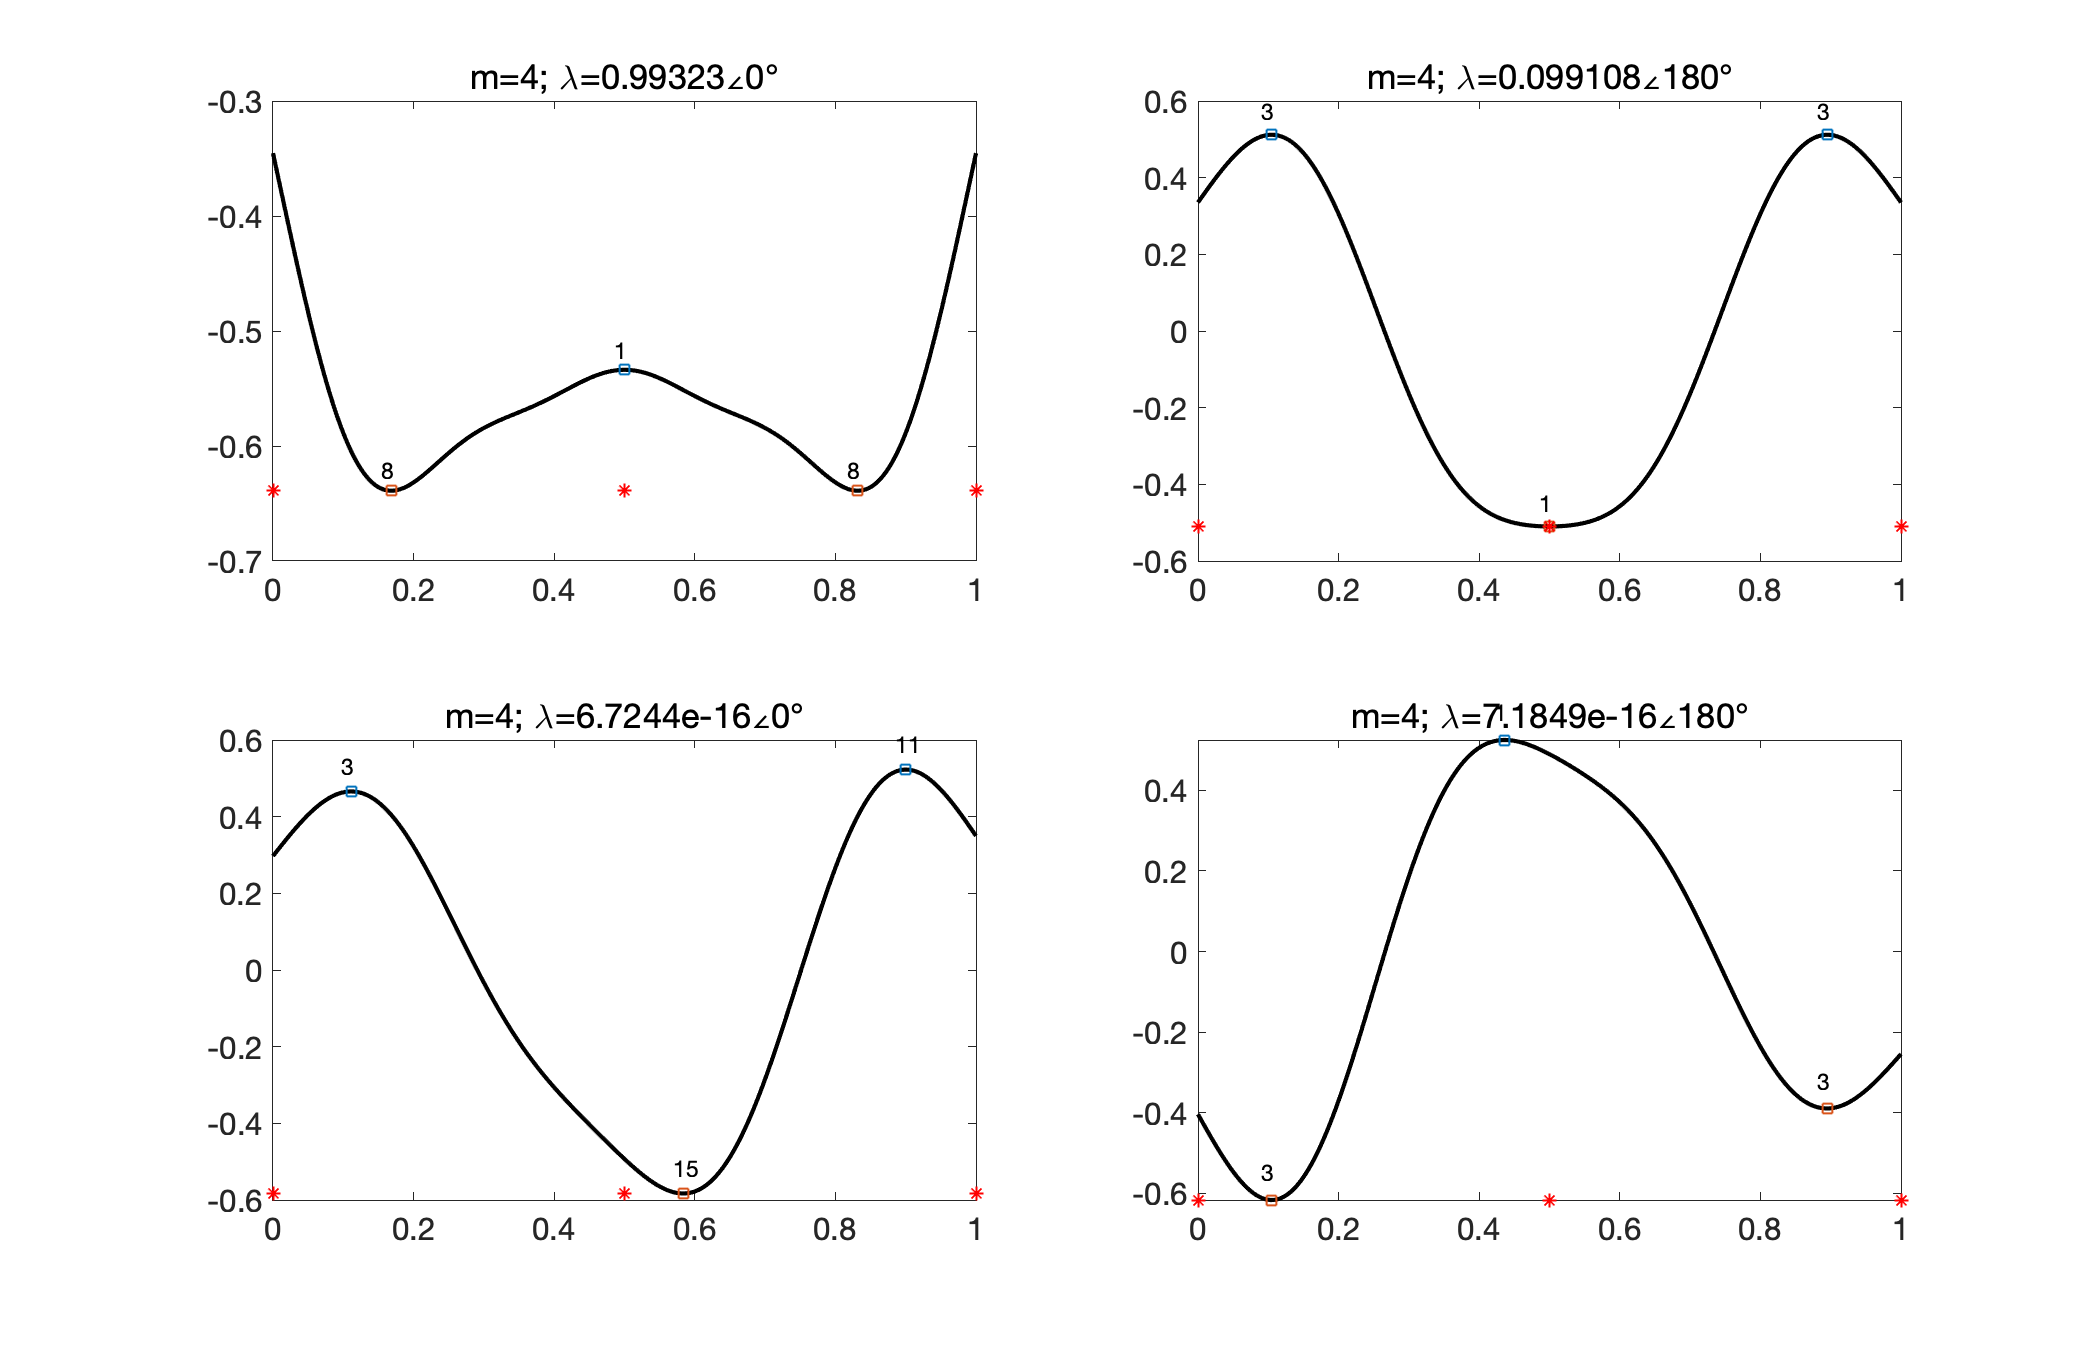
\includegraphics[scale=0.2]{tent/accurate/Tent_auto_level_n1000_m4}}
  \subfloat[m=8]{
    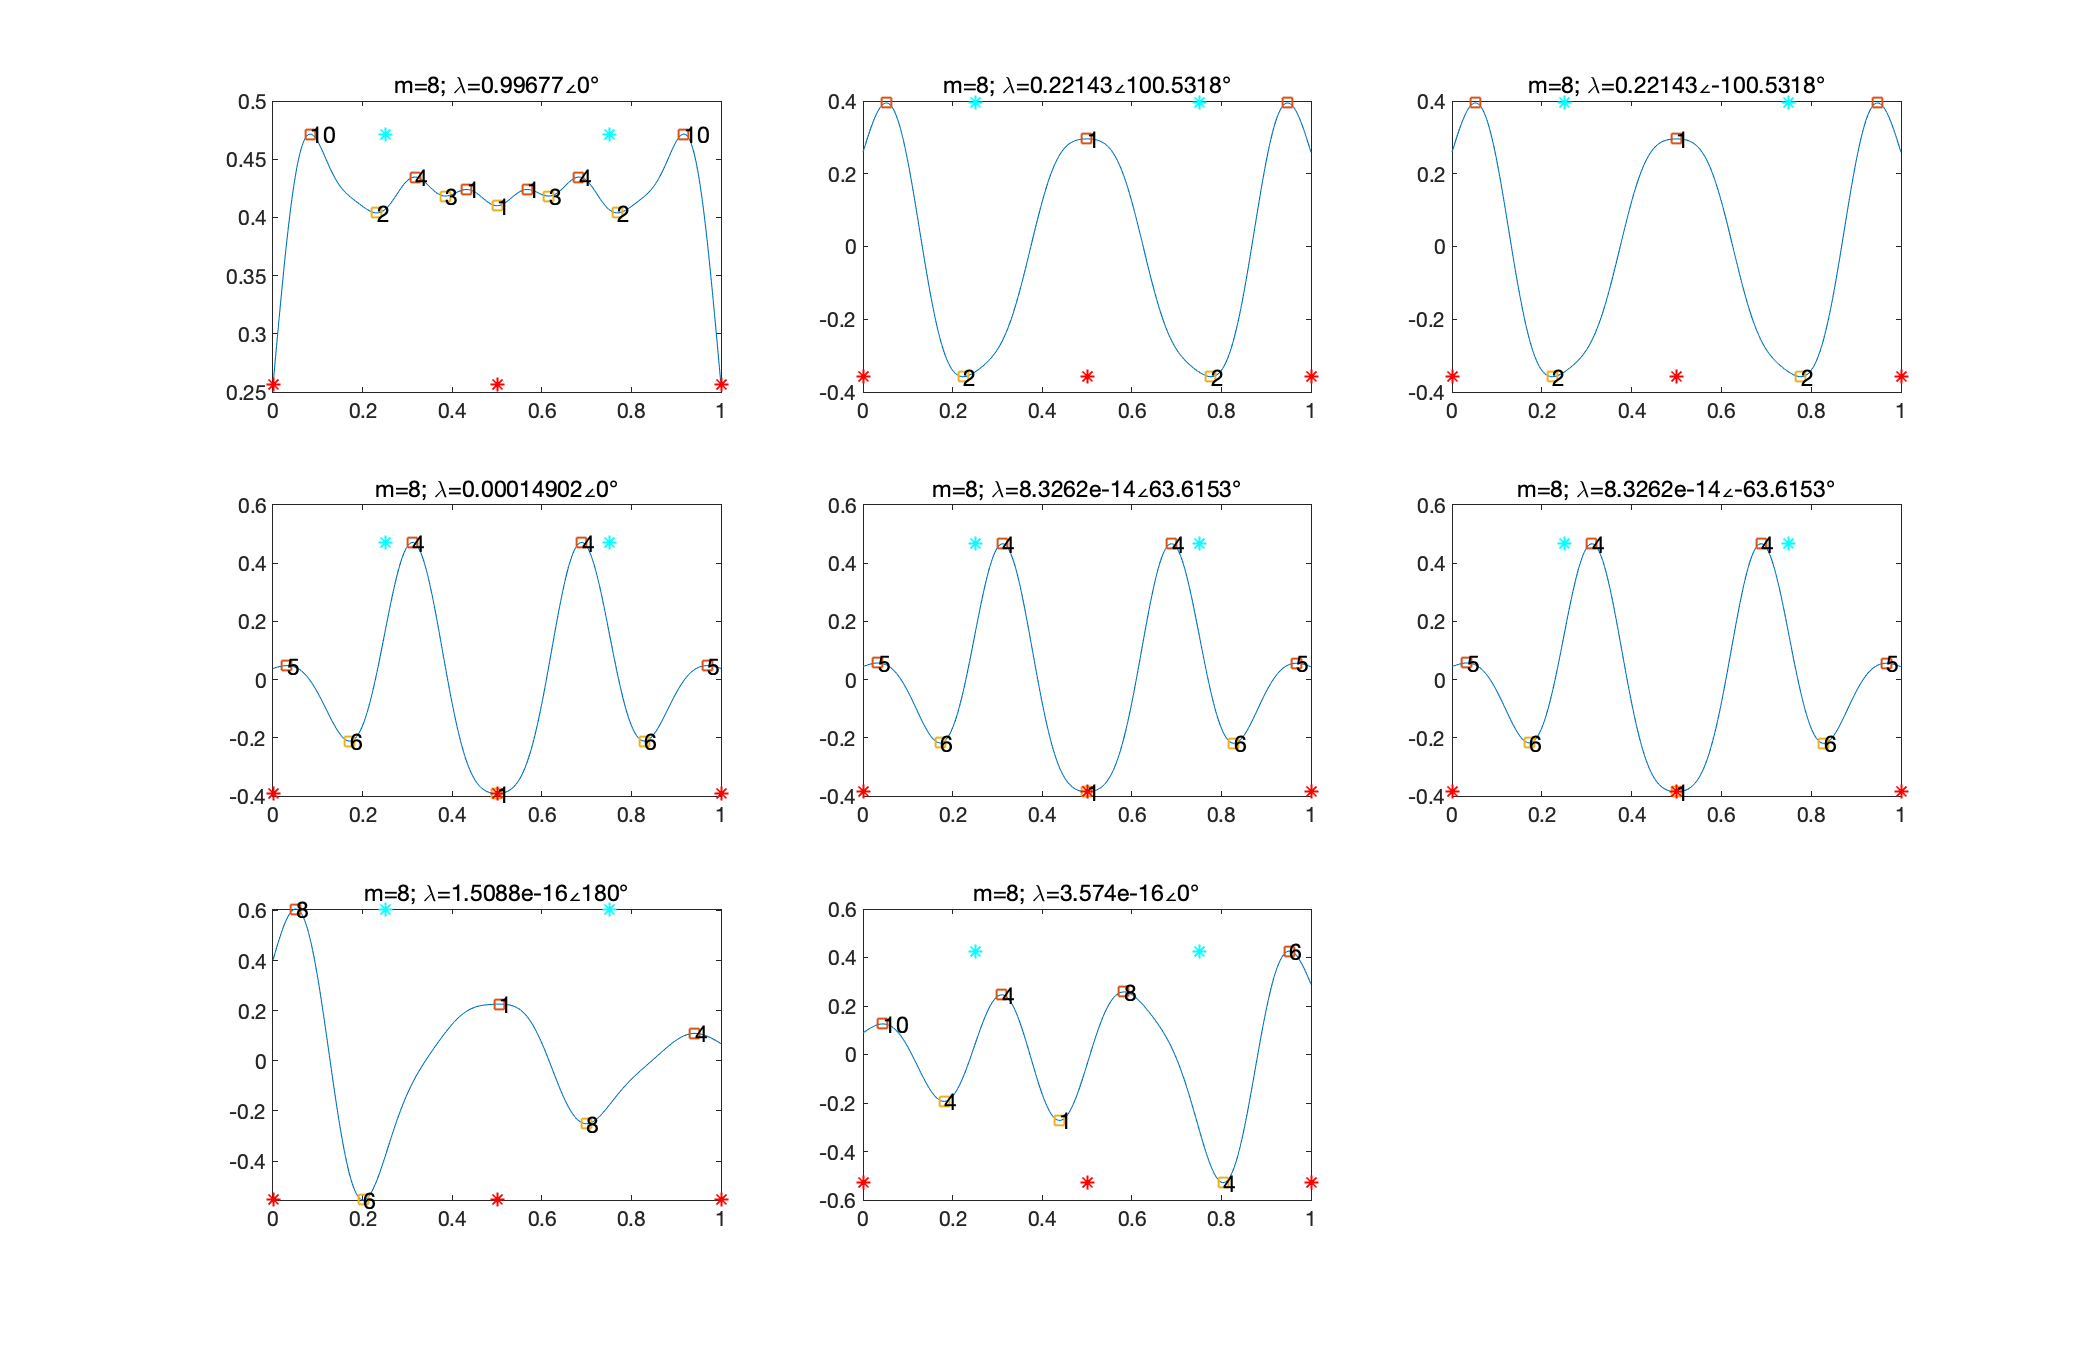
\includegraphics[scale=0.2]{tent/accurate/Tent_auto_level_n1000_m8}}
    \\
  \subfloat[m=10]{
    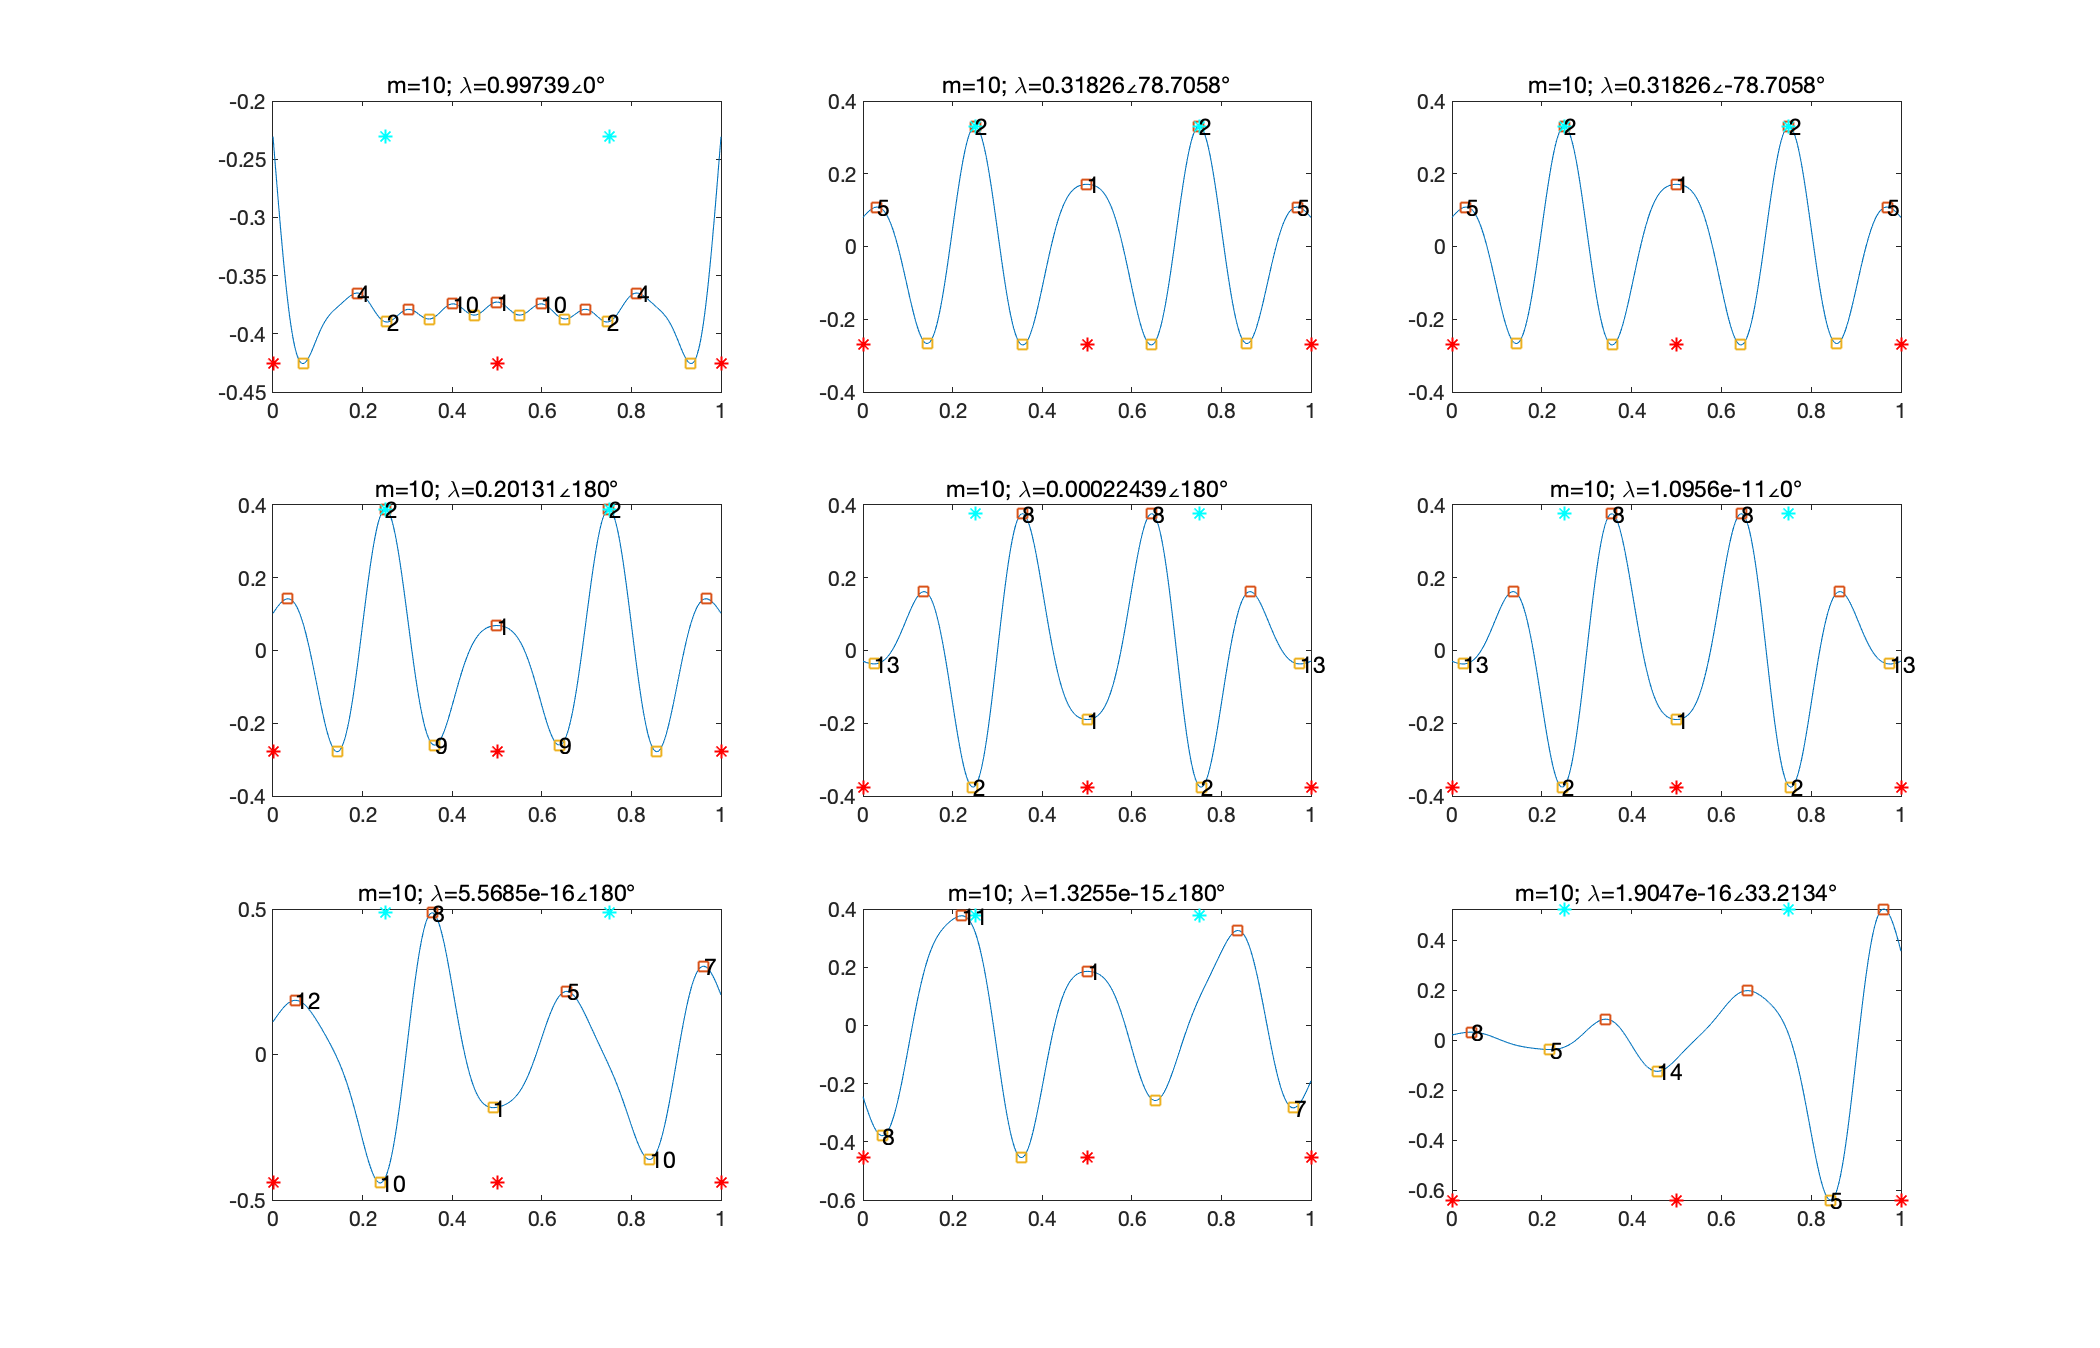
\includegraphics[scale=0.2]{tent/accurate/Tent_auto_level_n1000_m10}}
  \subfloat[m=20]{
    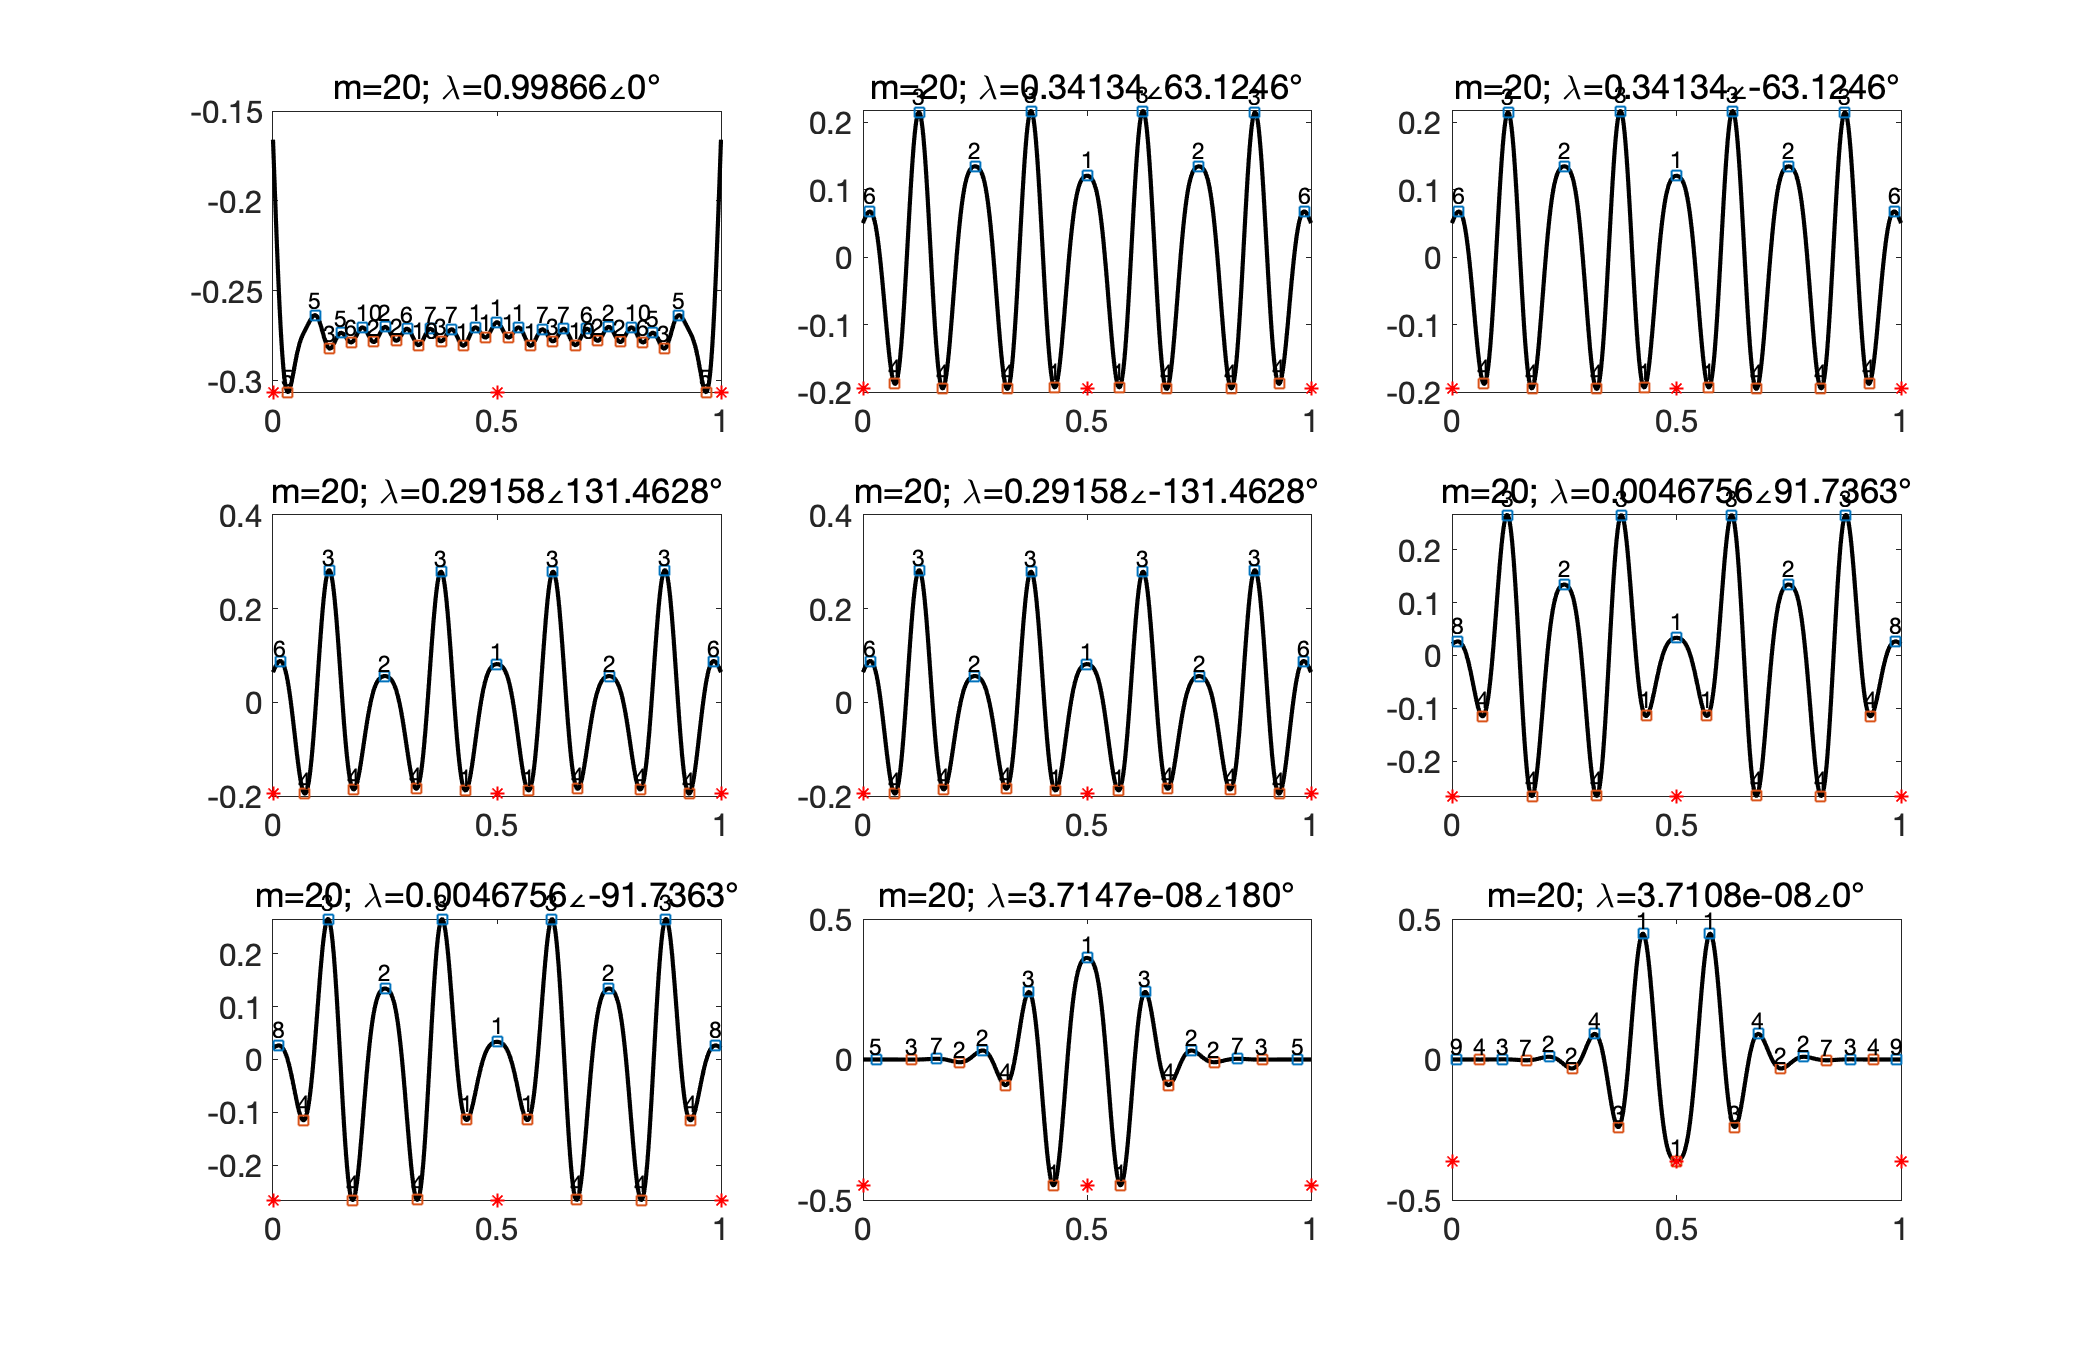
\includegraphics[scale=0.2]{tent/accurate/Tent_auto_level_n1000_m20}}
    \\
  \caption{帐篷映射本征函数确定边界点层次($n=1000$)}
\end{figure}

\begin{figure}
  \centering
  \subfloat[m=4]{
    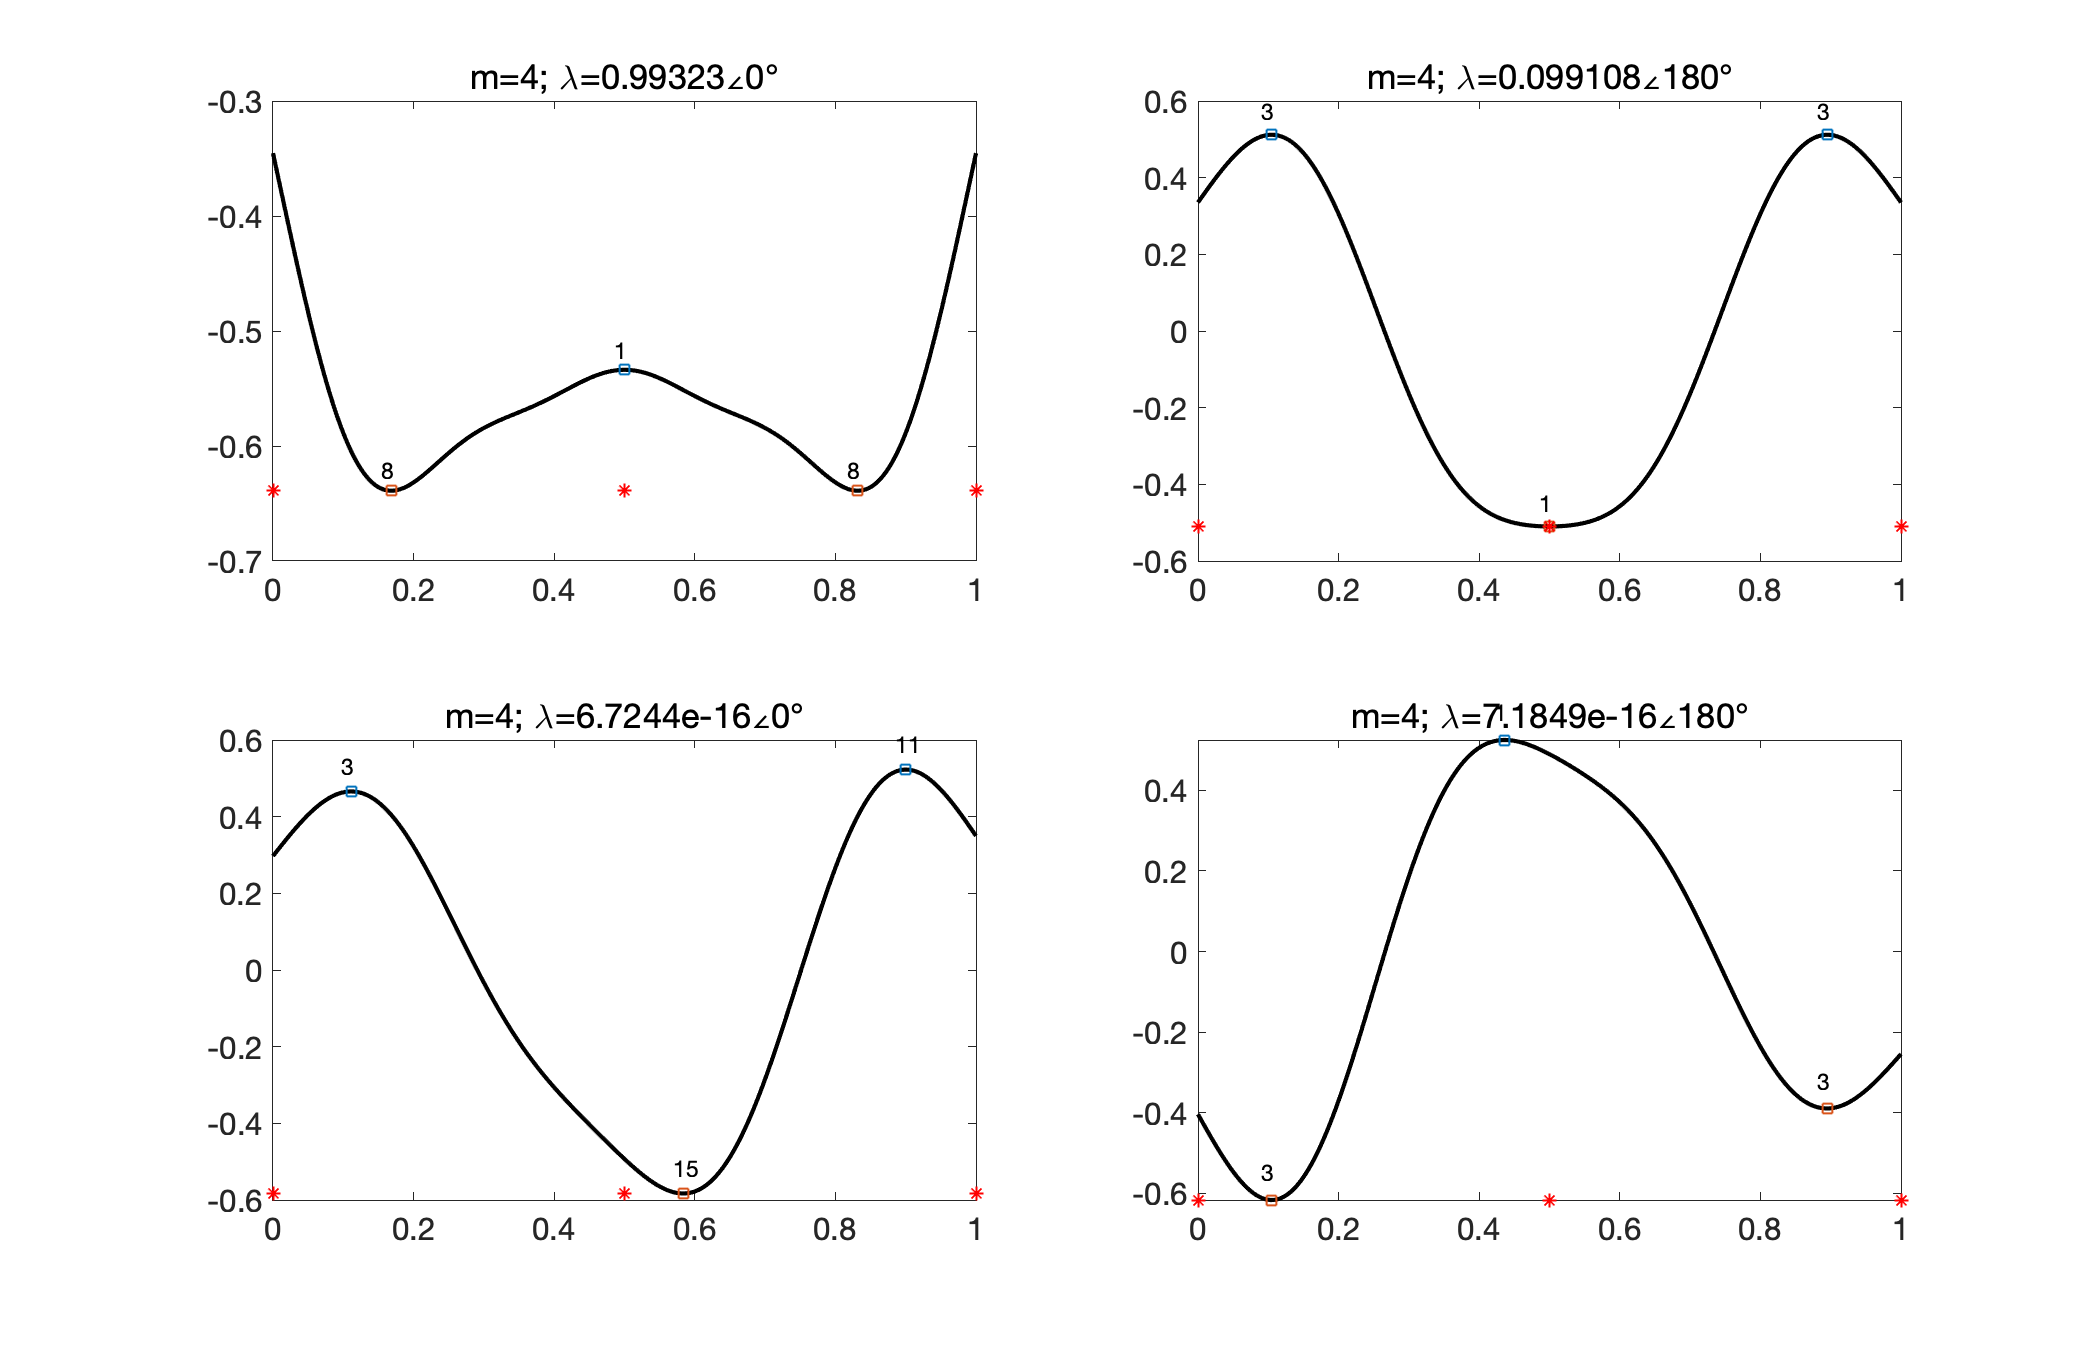
\includegraphics[scale=0.2]{tent/accurate/Tent_auto_level_n1000_m4}}
  \subfloat[m=8]{
    \includegraphics[scale=0.2]{tent/accurate/Tent_auto_level_n1000_m8}}
    \\
  \subfloat[m=10]{
    \includegraphics[scale=0.2]{tent/accurate/Tent_auto_level_n1000_m10}}
  \subfloat[m=20]{
    \includegraphics[scale=0.2]{tent/accurate/Tent_auto_level_n1000_m20}}
    \\
  \caption{帐篷映射本征函数确定边界点层次($noise=0$)}
\end{figure}

\begin{figure}
  \centering
  \subfloat[m=4]{
    \includegraphics[scale=0.2]{tent/accurate/Tent_autolevel_noise_n1000_m4}}
  \subfloat[m=8]{
    \includegraphics[scale=0.2]{tent/accurate/Tent_autolevel_noise_n1000_m8}}
    \\
  \subfloat[m=10]{
    \includegraphics[scale=0.2]{tent/accurate/Tent_autolevel_noise_n1000_m10}}
  \subfloat[m=20]{
    \includegraphics[scale=0.2]{tent/accurate/Tent_autolevel_noise_n1000_m20}}
    \\
  \caption{帐篷映射本征函数确定边界点层次($noise=0.001$)}
\end{figure}

\subsubsection{多峰映射}
\begin{figure}
  \centering
  \subfloat[noise=0]{
    \includegraphics[scale=0.2]{tent/tents/Tents5_noise_phase_d0}}
  \subfloat[noise=0.001]{
    \includegraphics[scale=0.2]{tent/tents/Tents5_noise_phase_d0-001}}
  \caption{双峰映射不同噪声下的相空间}
\end{figure}

\begin{figure}
  \centering%[2,3,4,5,8,10,15,20]
  \subfloat[m=2]{
    \includegraphics[scale=0.2]{tent/tents/Tents5_eigen_noise_n1000m2d0-001}}
  \subfloat[m=3]{
    \includegraphics[scale=0.2]{tent/tents/Tents5_eigen_noise_n1000m3d0-001}}
    \\
  \subfloat[m=4]{
    \includegraphics[scale=0.2]{tent/tents/Tents5_eigen_noise_n1000m4d0-001}}
  \subfloat[m=5]{
    \includegraphics[scale=0.2]{tent/tents/Tents5_eigen_noise_n1000m5d0-001}}
    \\
  \subfloat[m=8]{
    \includegraphics[scale=0.2]{tent/tents/Tents5_eigen_noise_n1000m8d0-001}}
  \subfloat[m=10]{
    \includegraphics[scale=0.2]{tent/tents/Tents5_eigen_noise_n1000m10d0-001}}
    \\
  \subfloat[m=15]{
    \includegraphics[scale=0.2]{tent/tents/Tents5_eigen_noise_n1000m15d0-001}}
  \subfloat[m=20]{
    \includegraphics[scale=0.2]{tent/tents/Tents5_eigen_noise_n1000m20d0-001}}
    \\
    \caption{双峰映射的边界点与本征函数($noise=0.001$)}
\end{figure}

\begin{figure}
  \centering
  \subfloat[noise=0]{
    \includegraphics[scale=0.2]{tent/tents/Tents5l_noise_phase_d0}}
  \subfloat[noise=0.001]{
    \includegraphics[scale=0.2]{tent/tents/Tents5l_noise_phase_d0-001}}
  \caption{大小峰映射不同噪声下的相空间}
\end{figure}

\begin{figure}
  \centering%[2,3,4,5,8,10,15,20]
  \subfloat[m=2]{
    \includegraphics[scale=0.2]{tent/tents/Tents5l_eigen_noise_n1000m2d0-001}}
  \subfloat[m=3]{
    \includegraphics[scale=0.2]{tent/tents/Tents5l_eigen_noise_n1000m3d0-001}}
    \\
  \subfloat[m=4]{
    \includegraphics[scale=0.2]{tent/tents/Tents5l_eigen_noise_n1000m4d0-001}}
  \subfloat[m=5]{
    \includegraphics[scale=0.2]{tent/tents/Tents5l_eigen_noise_n1000m5d0-001}}
    \\
  \subfloat[m=8]{
    \includegraphics[scale=0.2]{tent/tents/Tents5l_eigen_noise_n1000m8d0-001}}
  \subfloat[m=10]{
    \includegraphics[scale=0.2]{tent/tents/Tents5l_eigen_noise_n1000m10d0-001}}
    \\
  \subfloat[m=15]{
    \includegraphics[scale=0.2]{tent/tents/Tents5l_eigen_noise_n1000m15d0-001}}
  \subfloat[m=20]{
    \includegraphics[scale=0.2]{tent/tents/Tents5l_eigen_noise_n1000m20d0-001}}
    \\
    \caption{大小峰映射的边界点与本征函数($noise=0.001$)}
\end{figure}

\subsection{小结}